% 16 Component Dirac Fermion Condensate Singlet Superfluid on 7+1 Deflating Spacetime
% REVTeX 4.2, Physical Review D, two-column.
%
% This file is self-contained: the reference list is embedded at the end, so that no
% BibTeX run is needed.  Build (three runs settle all cross references), from the
% directory Revision_Deflation/manuscript/ of the repository (the figures are read from ../figures/):
%
%     pdflatex "16 Component Dirac Fermion Condensate Singlet Superfluid on 7+1 Deflating Spacetime.tex"
%
% DO NOT EDIT THIS FILE BY HAND.  It is assembled by code/scripts/build_manuscripts.py
% from the source files in docs_src/manuscript/ (which it shares with the companion
% manuscript on the 4+4 deflating spacetime), and every computed number in a
% table is inserted by that script from the data files in data/ (see provenance/RP8_code_deflation).
\documentclass[aps,prd,twocolumn,floatfix,nofootinbib,longbibliography]{revtex4-2}

\usepackage{amsmath,amssymb,bm}
\usepackage{graphicx}
\usepackage{dcolumn}
\usepackage{array}
\usepackage{booktabs}
\usepackage{xcolor}
\usepackage[colorlinks=true,linkcolor=blue!50!black,citecolor=blue!50!black,urlcolor=blue!50!black]{hyperref}
\graphicspath{{../figures/}}
\raggedbottom
\hypersetup{pdftitle={16 Component Dirac Fermion Condensate Singlet Superfluid on 7+1 Deflating Spacetime},
  pdfauthor={Patrick Lee Nash}}
% the same source always gives the same PDF file (no time stamp, no random identifier)
\ifdefined\pdfinfoomitdate\pdfinfoomitdate=1 \pdftrailerid{}\pdfsuppressptexinfo=-1 \fi
\setcounter{topnumber}{3}
\setcounter{bottomnumber}{2}
\setcounter{totalnumber}{5}
\setcounter{dbltopnumber}{3}
\renewcommand{\topfraction}{0.9}
\renewcommand{\bottomfraction}{0.6}
\renewcommand{\textfraction}{0.08}
\renewcommand{\floatpagefraction}{0.9}
\renewcommand{\dbltopfraction}{0.9}
\renewcommand{\dblfloatpagefraction}{0.9}

% ---------------------------------------------------------------- macros
% the tag that marks every object of the spacetime of this paper
\newcommand{\tg}{1671d}
% the three rates of deflation (the names of the hypotheses: upright, never with a subscript), and their combinations
\newcommand{\gff}{\mathrm{g55}}
\newcommand{\gss}{\mathrm{g66}}
\newcommand{\gvv}{\mathrm{g77}}
\newcommand{\gsum}{\mathrm{gsum}}
\newcommand{\gsq}{\mathrm{gsq}}
\newcommand{\gprod}{\mathrm{gprod}}
\newcommand{\rt}{\mathrm{rate}_t}
\newcommand{\cff}{\mathrm{const5}}
\newcommand{\css}{\mathrm{const6}}
\newcommand{\cvv}{\mathrm{const7}}
\newcommand{\ct}{\mathrm{const}_t}
% deflating volume, clock, weighted field
\newcommand{\Vd}{V_d}
\newcommand{\td}{\tau_d}
\newcommand{\tpair}{\tau_{\mathrm{pair}}}
\newcommand{\hpsi}{\hat\psi}
\newcommand{\Eperp}{E_\perp}
\newcommand{\kd}{k_d}
\newcommand{\ud}{u_d}
\newcommand{\ncr}{n_{\mathrm{cr}}}
\newcommand{\Tdefl}{T_{\mathrm{defl}}}
\newcommand{\Swkb}{S_{\mathrm{WKB}}}
\newcommand{\Xid}{\Xi_d}
\newcommand{\Deq}{\Delta_{\mathrm{eq}}}
\newcommand{\Esh}{E_{\mathrm{sh}}}
\newcommand{\nex}{n_{\mathrm{ex}}}
\newcommand{\nEW}{n_{\mathrm{EW}}}
\newcommand{\vEW}{v_{\mathrm{EW}}}
\newcommand{\GN}{G_N}
\newcommand{\aGB}{\alpha_{\mathrm{GB}}}
\newcommand{\Lam}{\Lambda_8}
\newcommand{\cG}{\mathcal{G}}
\newcommand{\cH}{\mathcal{H}}
\newcommand{\cX}{\mathcal{X}}
% perturbations of ordinary space (Sec. XI): conformal time, conformal Hubble rate, metric functions of the synchronous
% gauge, sums over matter and radiation, gaps
\newcommand{\tcf}{\tau_{\mathrm{cf}}}
\newcommand{\Hcf}{H_{\mathrm{cf}}}
\newcommand{\He}{H_e}
\newcommand{\hsy}{h_{\mathrm{sy}}}
\newcommand{\etasy}{\eta_{\mathrm{sy}}}
\newcommand{\alsy}{\alpha_{\mathrm{sy}}}
\newcommand{\cD}{\mathcal{D}}
\newcommand{\cT}{\mathcal{T}}
\newcommand{\cP}{\mathcal{P}}
\newcommand{\cA}{\mathcal{A}}
\newcommand{\cE}{\mathcal{E}}
\newcommand{\cB}{\mathcal{B}}
\newcommand{\cZ}{\mathcal{Z}}
\newcommand{\cYM}{\mathcal{Y}_M}
\newcommand{\cYT}{\mathcal{Y}_T}
\newcommand{\cYS}{\mathcal{Y}_S}
\newcommand{\YHe}{Y_{\mathrm{He}}}
% the Vorton-Scalar and its parameters
\newcommand{\PhiVS}{\Phi_{\mathrm{VS}}}
\newcommand{\vVS}{v_{\mathrm{VS}}}
\newcommand{\gVS}{g_{\mathrm{VS}}}
\newcommand{\aVS}{\alpha_{\mathrm{VS}}}
\newcommand{\DVS}{D_{\mathrm{VS}}}
\newcommand{\lamVS}{\lambda_{\mathrm{VS}}}
\newcommand{\yVS}{y_{\mathrm{VS}}}
\newcommand{\GVS}{G_{\mathrm{VS}}}
\newcommand{\UVS}{U(1)_{\mathrm{VS}}}
% general
\newcommand{\kF}{k_F}
\newcommand{\EF}{E_F}
\newcommand{\Cm}{C^{-}}
\newcommand{\hh}{\mathsf{h}}
\newcommand{\MM}{\mathsf{M}}
\newcommand{\kmsMpc}{\mathrm{km\,s^{-1}\,Mpc^{-1}}}

\begin{document}

\title{16 Component Dirac Fermion Condensate Singlet Superfluid on 7+1 Deflating Spacetime}

\author{Patrick Lee Nash, Ph.D.}
\affiliation{Independent researcher}

\date{November 13, 2026}

\begin{abstract}
A 16-component Dirac field is studied on a spacetime with seven space-like dimensions and one
time-like dimension in which three of the space-like coordinates deflate exponentially as time
advances. We derive the geometry, the spin connection and the Dirac equation, and solve the equation
exactly. The deflation creates particles in every mode that depends on a deflating coordinate, with a
Fermi-Dirac spectrum whose temperature is the rate divided by $2\pi$. Fields that do not depend on the
deflating coordinates obey the flat equations with couplings that grow with the deflation. The
superfluid of fermion pairs bound by the Vorton-Scalar therefore acquires a history: its gap grows
much faster than the coupling, two fermions become bound at a scattering resonance, and the paired
state follows the deflation only once its gap exceeds a few times the rate divided by the pairing
strength. With equal rates the spacetime is an exact vacuum solution of Einstein-Gauss-Bonnet gravity.
If gravity feels the deflation, the Hubble constant inferred from the microwave background falls.
The rotations that would make the pair condensate a Higgs field are no longer symmetries of the
spacetime, and if the superfluid were the Higgs field, atomic clocks would limit the rate of deflation
to a millionth of the Hubble rate.
\end{abstract}

\maketitle

\section{Introduction}
\label{sec:intro}

\subsection{The question}

Two earlier papers \cite{Flat1644,Flat1671} studied a single fermion field with sixteen components on
two flat spacetimes of eight dimensions. One has four space-like and four time-like dimensions, and is
written $4{+}4$; the other has seven space-like dimensions and one time-like dimension, and is written
$7{+}1$. On both, the eight Dirac matrices can be chosen real, and the field supports a superfluid of
fermion pairs whose order parameter points along one of the four coordinates that are not the
coordinates of ordinary spacetime. This paper treats the $7{+}1$ spacetime; a companion paper
\cite{CompanionDefl1644} treats $4{+}4$.

The eight coordinates are written $x0,x1,\dots,x7$. Throughout, $x1,x2,x3$ are the coordinates of
ordinary space and $x4$ is the ordinary time. The coordinate $x0$ is an additional space-like
coordinate, called the hidden coordinate. The remaining three, $x5,x6,x7$, are
three additional \emph{space-like} coordinates.

In the flat theory nothing explains why the fields of ordinary physics do not depend on $x5$, $x6$
and $x7$. On the $7{+}1$ spacetime
this was an assumption of the earlier paper. The present paper examines a definite proposal for what
happens to these three coordinates.

\subsection{The hypothesis of deflation}

The hypothesis is that \emph{the coordinates $x5$, $x6$ and $x7$ deflate exponentially}: as the
ordinary time $x4$ advances, the proper extent of every interval along each of these coordinates
shrinks as an exponential of $x4$. Flat spacetime is replaced by a curved spacetime with a diagonal
metric, in which the three components of the metric along the deflating coordinates are
\begin{equation}
\begin{aligned}
g_{55}&=-\cff^{2}\,e^{-2\,\gff\,x4},\\
g_{66}&=-\css^{2}\,e^{-2\,\gss\,x4},\\
g_{77}&=-\cvv^{2}\,e^{-2\,\gvv\,x4}.
\end{aligned}
\label{eq:hyp}
\end{equation}
Here $\gff$, $\gss$ and $\gvv$ are three positive constants, the \emph{rates} of deflation; $\cff$,
$\css$ and $\cvv$ are three positive constants that set the scale at $x4=0$. The names of the rates
are written upright and without a subscript, to distinguish them from the components $g_{55}$,
$g_{66}$, $g_{77}$ of the metric, which carry subscripts. The other five components of the metric
keep their flat values. The minus signs in
Eq.~(\ref{eq:hyp}) are those of space-like components in the convention of this paper, in which the
time-like component is positive.

The earlier papers examined three hypotheses about the superfluid, and we keep their labels.
\begin{itemize}
\item[H1.] The fermion field forms a superfluid state of spin 0 in which the fermions are paired by
the exchange of a new scalar boson, the \emph{Vorton-Scalar}, through a neutral current of the kind
known from the weak interaction.
\item[H2.] This superfluid state is the Higgs field.
\item[H3.] This superfluid state explains the observations of dark matter, or the Hubble tension, or
both.
\end{itemize}
The purpose of this paper is to repeat every calculation of the earlier paper under the hypothesis of
deflation, and to report what changes for H1, H2 and H3, favorable or not.

\subsection{Summary of results}

\emph{Geometry} (Sec.~\ref{sec:geometry}). The deflating spacetime is homogeneous and has 14
symmetries, or 15 or 20 if two or three of the rates are equal, instead of the 36 of flat spacetime.
It is not a solution of Einstein's equations without matter. With three equal rates it \emph{is} an
exact solution of the equations of Einstein-Gauss-Bonnet gravity without matter, for one definite
relation between the rate and the two constants of that theory.

\emph{The Dirac field} (Secs.~\ref{sec:dirac}, \ref{sec:modes}). A field that does not depend on
$x5,x6,x7$ obeys, after multiplication by the square root of the volume factor of the deflating
coordinates, exactly the flat equation. A field that does depend on them is affected directly.
We solve its equation exactly. \emph{The deflation creates particles}: a mode that starts empty ends
with the occupation of a Fermi-Dirac distribution at a temperature equal to the rate divided by
$2\pi$, the Gibbons-Hawking temperature of the de Sitter space that the deflating coordinates and the
time form when the rates are equal.

\emph{The superfluid} (Secs.~\ref{sec:clock} to \ref{sec:order}). For fields that do not depend on
the extra coordinates the model of the earlier paper holds unchanged, with one difference: its
coupling grows with the time, because a coupling of the four-dimensional description is a coupling
of the eight-dimensional theory divided by a power of the deflating volume. The masses do not change.
Every threshold of the earlier paper is therefore passed at a definite time. The gap of the paired
state grows much faster than the coupling. Two fermions become bound at a scattering resonance. The
paired state can follow the deflation only once its gap exceeds a few times the rate divided by the
pairing strength; before that it lags behind and breaks pairs. Matter of a given density loses its
fermion mass at a definite time. A vortex line carries four fermion zero modes.

\emph{Cosmology} (Sec.~\ref{sec:cosmo}). If gravity is the Einstein theory in eight dimensions,
Newton's constant grows at the total rate of deflation; lunar laser ranging then bounds that rate to
$3\times10^{-3}$ of the Hubble rate, and the Hubble constant inferred from the microwave background
falls. The deflation does not relieve the Hubble tension. Whatever keeps the rates constant must
carry a tension and must take part in the perturbations of ordinary space; the spectra of the
microwave background at all but the largest angular scales do not depend on how it does so, and
the growth of structure does.

\emph{The Higgs hypothesis} (Sec.~\ref{sec:higgs}). The rotations of the four extra space-like coordinates, under which the pair condensate
has the pattern of the Higgs vacuum, are no longer symmetries of the spacetime; the pattern survives
only as a hidden symmetry. If the condensate were the Higgs field, the electroweak scale would follow
the growing coupling, and atomic clocks would limit the rate of deflation to about $10^{-6}$ of the
Hubble rate. The hypothesis H2 and a deflation of any consequence today exclude each other.

\subsection{Method, and the limits of what is claimed}

Every statement of this paper about geometry, matrices and operators is an identity that a program
has verified in exact rational arithmetic, and that an independent program has verified again by
computer algebra for arbitrary values of the rates. Every numerical statement is the output of a
program, with a stated accuracy. The programs, their output and the documents that derive each result
step by step are public \cite{DeflationRepo}; the program performs 238 checks, all of which
pass. The metric of Eq.~(\ref{eq:hyp}) is a hypothesis. The paper derives its consequences; it does
not claim that the hypothesis is true. Section~\ref{sec:status} lists what has been established and
what has not.

Units are natural, $\hbar=c=k_B=1$. Symbols that carry the tag $\tg$ refer to the deflating
$7{+}1$ spacetime. A general coordinate among the three deflating ones is written $xt$ with
$t\in\{5,6,7\}$ and its rate $\rt$; a general coordinate among $x0,x1,x2,x3$ is written $xj$ with $j\in\{0,1,2,3\}$. The letter $a$ is kept for the four extra axes, $a\in\{0,5,6,7\}$ (Sec.~\ref{sec:gap}).
Appendix~\ref{app:symbols} lists the symbols.

\section{The deflating spacetime}
\label{sec:geometry}

This section derives the geometry that the hypothesis implies: the curvature, the field equations
that the metric does and does not solve, its symmetries, and the motion of a classical particle. The
derivations are given in full in Ref.~\cite{DeflationRepo}.

\subsection{Metric, frame and volume}

Let $\eta=\mathrm{diag}(-1,-1,-1,-1,+1,-1,-1,-1)$ be the flat metric
of the earlier paper, with the coordinates in the order $x0,\dots,x7$. Define three \emph{scale
factors}, one for each deflating coordinate,
\begin{equation}
b_t(x4)=\ct\,e^{-\rt\,x4},\qquad t=5,6,7,
\label{eq:scale}
\end{equation}
with $\mathrm{rate}_5=\gff$, $\mathrm{rate}_6=\gss$, $\mathrm{rate}_7=\gvv$. The metric of the
deflating spacetime is
\begin{equation}
g_{\mu\nu}=\mathrm{diag}\big(\eta_{00},\eta_{11},\eta_{22},\eta_{33},\eta_{44},\,\eta_{55}b_5^2,\,\eta_{66}b_6^2,\,\eta_{77}b_7^2\big),
\label{eq:metric}
\end{equation}
whose last three components are those of Eq.~(\ref{eq:hyp}). Greek indices label the coordinates. A
coordinate interval $dxt$ has the proper extent $b_t\,|dxt|$, which shrinks by the factor $e$ in the
time $1/\rt$. Because $x5,x6,x7$ are space-like, what shrinks is a length.

Capital indices $A,B$ label an orthonormal frame, eight vector fields $e_A=e_A{}^{\mu}\partial_\mu$
with $g_{\mu\nu}e_A{}^{\mu}e_B{}^{\nu}=\eta_{AB}$. We take the frame along the coordinates,
$e_A{}^{\mu}=\mathrm{diag}(1,1,1,1,1,b_5^{-1},b_6^{-1},b_7^{-1})$. The volume element is $\Vd\,d^8x$
with
\begin{equation}
\Vd(x4)=b_5b_6b_7\propto e^{-\gsum\,x4},\quad\gsum=\gff+\gss+\gvv .
\label{eq:Vd}
\end{equation}
$\Vd$ is the proper volume of a unit coordinate cell of the deflating coordinates, and the
\emph{total rate} $\gsum$ is the rate at which it shrinks. Most results below depend on the three
rates only through $\gsum$.

\subsection{Curvature}
\label{sec:curvature}

The only components of the metric that depend on a coordinate are the three $g_{tt}$, and they depend
on $x4$ alone. The Christoffel symbols that do not vanish are
\begin{equation}
\Gamma^{t}{}_{4t}=-\rt,\qquad\Gamma^{4}{}_{tt}=\eta_{44}\eta_{tt}\,\rt\,b_t^{2},
\end{equation}
without summation over $t$. The Riemann tensor has, in the orthonormal frame, the components
\begin{equation}
R^{t}{}_{4t4}=-\rt^{2},\quad R^{t}{}_{sts}=-\eta_{44}\eta_{ss}\,\rt\,\mathrm{rate}_s\ \ (t\ne s),
\label{eq:riemann}
\end{equation}
and those related to them by symmetry. No component carries an index of $x0,\dots,x3$: these four
coordinates span a flat space, and the curvature lives in the four coordinates $x4,\dots,x7$. With
$\gsq=\gff^2+\gss^2+\gvv^2$ and $\gprod=\gff\gss+\gff\gvv+\gss\gvv$, the curvature scalar is the
constant $R=-\eta_{44}(\gsq+\gsum^{2})$, and the Einstein tensor
$\cG^{\mu}{}_{\nu}=R^{\mu}{}_{\nu}-\tfrac12R\,\delta^{\mu}_{\nu}$ is diagonal with
\begin{equation}
\begin{aligned}
\cG^{4}{}_{4}&=\eta_{44}\,\gprod,\qquad\cG^{j}{}_{j}=\tfrac12\eta_{44}\,(\gsq+\gsum^{2}),\\
\cG^{t}{}_{t}&=\eta_{44}\big[\tfrac12(\gsq+\gsum^{2})-\rt\,\gsum\big].
\end{aligned}
\label{eq:einstein}
\end{equation}
The Einstein tensor does not vanish, and it is not a multiple of the unit matrix unless all rates
vanish. \emph{The deflating spacetime is not a solution of Einstein's equations without matter, with
or without a cosmological constant.}

\subsection{A solution of Einstein-Gauss-Bonnet gravity}
\label{sec:egb}

In more than four dimensions the general field equations of second order for the metric are those of
Lovelock \cite{Lovelock1971}. Their first term beyond Einstein's is the Lanczos tensor
$\cH^{\mu}{}_{\nu}$ of the Gauss-Bonnet term \cite{BoulwareDeser1985}, and the equations without
matter read
\begin{equation}
\cG^{\mu}{}_{\nu}+\Lam\,\delta^{\mu}_{\nu}+\aGB\,\cH^{\mu}{}_{\nu}=0,
\label{eq:egb}
\end{equation}
with a cosmological constant $\Lam$ and a coupling $\aGB$. (In this subsection the signs are those of
the convention in which space-like components of the metric are positive.) For the metric
(\ref{eq:metric}) we find
\begin{equation}
\begin{aligned}
\cH^{j}{}_{j}&=-4\,\gff\,\gss\,\gvv\,\gsum\quad(j=0,1,2,3),\\
\cH^{4}{}_{4}&=\cH^{t}{}_{t}=0,
\end{aligned}
\label{eq:lanczos}
\end{equation}
and the Lovelock tensor of the third order, the last that can differ from zero in eight dimensions,
vanishes identically. The components of Eq.~(\ref{eq:egb}) along $x4,\dots,x7$ therefore contain no
Gauss-Bonnet term and require the four corresponding components of the Einstein tensor to be equal,
which holds if and only if the three rates are equal. The components along $x0,\dots,x3$ then fix the
coupling. The result:
\begin{equation}
\gff=\gss=\gvv:\qquad\Lam=3\,\gff^{2},\qquad\aGB=-\frac{1}{4\,\gff^{2}} .
\label{eq:egbsol}
\end{equation}
\emph{With three equal rates the deflating spacetime is an exact solution of Einstein-Gauss-Bonnet
gravity without matter}, in a theory whose two constants satisfy $4\aGB\Lam=-3$; the rate is then
$\gff=\sqrt{\Lam/3}$. With unequal rates it is not a solution for any $\Lam$ and $\aGB$. Solutions of
this theory in which every scale factor is an exponential of the time have been classified in five
and six dimensions \cite{ChirkovPavluchenkoToporensky2014}; the present one, with four static and
three contracting directions in eight dimensions, is of that kind. Whether it is stable has not been
examined.

\subsection{Symmetries}

A Killing vector is a vector field along which the metric does not change. Flat spacetime in eight
dimensions has 36. The deflating spacetime has, for any rates, 14: the seven translations along all
coordinates but $x4$; the six rotations of $x0,x1,x2,x3$; and the scaling
\begin{equation}
\cX_{\mathrm{scale}}=\partial_4+\gff\,x5\,\partial_5+\gss\,x6\,\partial_6+\gvv\,x7\,\partial_7,
\label{eq:scaling}
\end{equation}
which shifts the time and stretches the deflating coordinates so as to undo the shrinking. Two equal
rates add the rotation of the two coordinates concerned. Three equal rates add the three rotations of
$x5,x6,x7$ and three further vectors, 20 in all; the four coordinates $x4,\dots,x7$ then form a space
of constant curvature of radius $1/\gff$:
de Sitter space in the half of its flat slicing in
which space contracts. These lists are complete. (A Killing vector that vanishes at a point is a
Lorentz transformation of the tangent space that leaves the Riemann tensor (\ref{eq:riemann})
unchanged; the dimension of the space of such transformations is 6, 7 or 12, which bounds the number
of Killing vectors by 14, 15 or 20.)

Three consequences are used below. The spacetime is homogeneous: no place and no moment is
distinguished. The constants $\ct$ are not observable by themselves, since a rescaling of $xt$
changes them; the deflation is observable only through an object that fixes a coordinate scale along
$xt$, such as a wave of given coordinate wavelength. And there is no conserved energy, because a
translation in time alone is not a symmetry.

Of the 28 rotations and boosts of flat spacetime, only the six rotations of $x0,\dots,x3$ survive for
general rates (Fig.~\ref{fig:isometries}). Nothing that involves the time survives, in particular
not the boosts of ordinary special relativity: the deflation defines a preferred state of rest, as
the expansion of the universe does.

\begin{figure*}
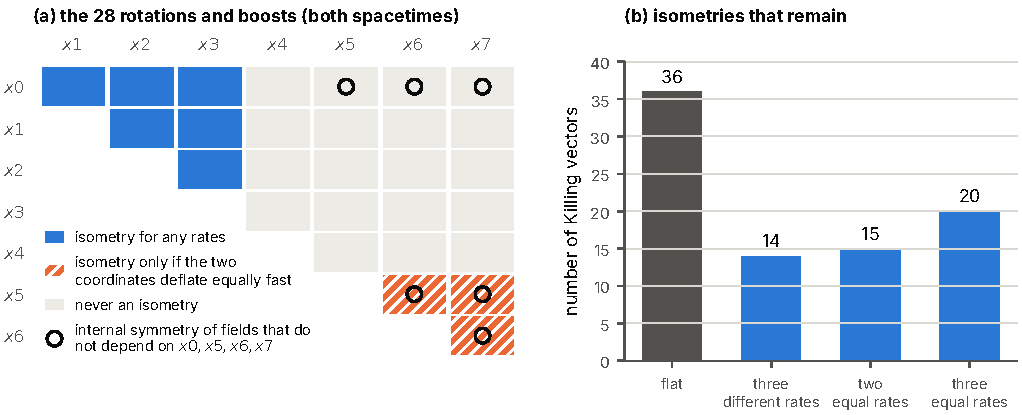
\includegraphics[width=0.86\textwidth]{fig_isometries}
\caption{\label{fig:isometries}Symmetries of the deflating spacetime. (a) The 28 rotations and boosts
of flat spacetime, one square for each pair of coordinates: those that remain symmetries for any
rates, those that remain symmetries only if the two coordinates deflate equally fast, and those that
are never symmetries. Circles mark the six pairs whose rotations act as internal symmetries on fields
that do not depend on $x0,x5,x6,x7$ (Sec.~\ref{sec:higgs}). (b) The number of Killing vectors.}
\end{figure*}

\subsection{Geodesics}
\label{sec:geodesics}

The translations give seven conserved momenta $P_\mu$ ($\mu\ne4$) of a classical particle. Let
$\Eperp=(m^{2}+\sum_jP_j^{2})^{1/2}$, with the sum over $j=0,1,2,3$, be the energy that a particle of
mass $m$ would have without momentum along the deflating coordinates. The conservation of the norm of the momentum gives the
velocity along the time, with an affine parameter $\varsigma$ along the path:
\begin{equation}
\Big(\frac{dx4}{d\varsigma}\Big)^{2}=\Eperp^{2}+\sum_{t}\frac{P_t^{2}}{b_t(x4)^{2}} .
\label{eq:geodesic}
\end{equation}
The last term grows as $e^{2\,\rt\,x4}$: the momentum $P_t$ belongs to a fixed coordinate wavelength,
and the proper wavelength shrinks.
With the plus sign the energy of a particle that moves along a deflating coordinate grows without
bound, the reverse of the redshift in an expanding universe. For momentum along $x5$ alone the proper
time that elapses between $x4$ and $x4=\infty$ is
\begin{equation}
\frac{m}{\gff\,\Eperp}\,\mathrm{arsinh}\Big(\frac{\Eperp\,\cff\,e^{-\gff\,x4}}{|P_5|}\Big),
\label{eq:incomplete}
\end{equation}
which is finite [Fig.~\ref{fig:geodesics}(a)]: the coordinates of Eq.~(\ref{eq:metric}) do not cover
the whole future of such a particle. For equal rates this is the known incompleteness of the flat slicing of de Sitter space.
Section~\ref{sec:modes} shows the quantum form of the blueshift. (On the $4{+}4$ spacetime the sign is
the opposite, and such a particle is turned back \cite{CompanionDefl1644}.)

\begin{figure*}
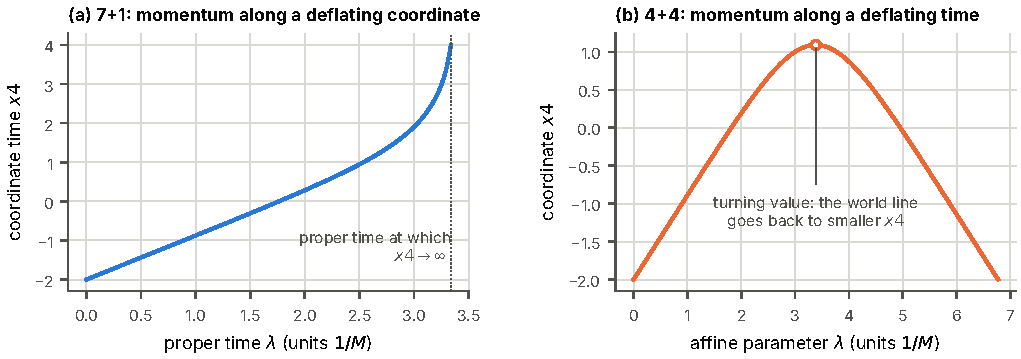
\includegraphics[width=0.8\textwidth]{fig_geodesics}
\caption{\label{fig:geodesics}A classical particle of the mass $m=1$ with the momenta $P_1=0.5$ along
$x1$ and $P_5=0.3$ along the deflating coordinate $x5$, for $\gff=1$ and $\cff=0.8$, started at
$x4=-2$. (a) On the $7{+}1$ spacetime the time $x4$ grows without bound within the finite proper time
3.386. (b) On the $4{+}4$ spacetime the path reaches the turning value $x4=1.0924$ and returns to
smaller $x4$.}
\end{figure*}

\section{The Dirac field}
\label{sec:dirac}

\subsection{Matrices and spin connection}

At each point of a curved spacetime the tangent space is flat. The Dirac matrices of the orthonormal
frame are therefore the eight real $16\times16$ matrices $\gamma^{A}$ of the earlier paper
\cite{Flat1671}, which satisfy $\gamma^{A}\gamma^{B}+\gamma^{B}\gamma^{A}=2\eta^{AB}$;
all of their properties were verified again for this work. The matrices with a coordinate index are
$\gamma^{\mu}=e_A{}^{\mu}\gamma^{A}$: five of them are the constant matrices, and the three along the
deflating coordinates are the constant matrices divided by the scale factors, $\gamma^{A=t}/b_t$.
They satisfy $\gamma^{\mu}\gamma^{\nu}+\gamma^{\nu}\gamma^{\mu}=2g^{\mu\nu}$.

A spinor is defined relative to a frame, and its derivative must account for the turning of the frame
from point to point \cite{BrillWheeler1957}. The covariant derivative of a spinor is
$\nabla_\mu\psi=(\partial_\mu+\Omega_\mu)\psi$ with the spin connection
$\Omega_\mu=\tfrac14\omega_{\mu AB}\gamma^{A}\gamma^{B}$, whose coefficients follow from the metric.
For the metric (\ref{eq:metric}) the only coefficients that do not vanish are
$\omega_{t\,t4}=-\omega_{t\,4t}=-\eta_{tt}\,\rt\,b_t$, so that
\begin{equation}
\begin{aligned}
\Omega_t&=-\tfrac12\,\eta_{tt}\,\rt\,b_t\,\gamma^{t}\gamma^{4}\quad(t=5,6,7),\\
\Omega_0&=\dots=\Omega_4=0,
\end{aligned}
\label{eq:spinconn}
\end{equation}
with the constant matrices of the frame on the right. Each $\Omega_t$ generates the Lorentz
transformation in the plane of $xt$ and $x4$. The spin connection is correct if and only if the
Dirac matrices are covariantly constant,
$\partial_\mu\gamma^{\nu}+\Gamma^{\nu}{}_{\mu\lambda}\gamma^{\lambda}+[\Omega_\mu,\gamma^{\nu}]=0$,
which holds for all 64 pairs of indices. Its curvature is the Riemann tensor,
$[\nabla_\mu,\nabla_\nu]\psi=\tfrac14R_{AB\mu\nu}\gamma^{A}\gamma^{B}\psi$, a third route to
Eq.~(\ref{eq:riemann}). One combination enters the Dirac equation:
\begin{equation}
\gamma^{\mu}\Omega_\mu=-\tfrac12\,\gsum\,\gamma^{4} .
\label{eq:gammaomega}
\end{equation}
The scale factors cancel, and only the total rate remains.

\subsection{The Dirac equation}

The field of this paper, $\psi_{\tg}(x)$, is a column of sixteen complex-valued Grassmann operators.
Its equation is the equation of the earlier paper with the covariant derivative and the matrices
$\gamma^{\mu}$:
\begin{equation}
\big(i\gamma^{\mu}\nabla_\mu-m\big)\psi_{\tg}=0 .
\label{eq:dirac}
\end{equation}
With Eq.~(\ref{eq:gammaomega}),
\begin{equation}
i\gamma^{4}\Big(\partial_4-\frac{\gsum}{2}\Big)\psi+i\sum_{j=0}^{3}\gamma^{j}\partial_j\psi
+i\sum_{t=5}^{7}\frac{\gamma^{t}}{b_t}\,\partial_t\psi-m\,\psi=0,
\label{eq:diracexp}
\end{equation}
with the constant matrices. Two things have changed with respect to flat spacetime: the derivative
along the time is shifted by $\gsum/2$, and each derivative along a deflating coordinate is divided
by its scale factor.

\subsection{The weighted field}

The shift is removed by a change of normalization. Define the \emph{weighted field}
\begin{equation}
\hpsi=\sqrt{\Vd}\,\psi .
\label{eq:weighted}
\end{equation}
Because $\partial_4\sqrt{\Vd}=-\tfrac12\gsum\sqrt{\Vd}$, the weighted field obeys
Eq.~(\ref{eq:diracexp}) without the term $\gsum/2$. The quantity $\psi^\dagger\psi$ is a density per
unit of proper volume and grows as the deflating coordinates shrink; $\hpsi^\dagger\hpsi$ is the
density per unit of coordinate volume, from which this trivial growth is removed.

The central observation of this paper follows at once. \emph{For a field that does not depend on
$x5$, $x6$, $x7$, the equation of the weighted field is exactly the flat equation.} Every result of
the earlier paper for such fields, in particular everything about the pairing of the fermions, holds
for the weighted field. The deflation enters those results in one way only, through the dependence of
the couplings on $\Vd$ (Sec.~\ref{sec:clock}).

A field that does depend on a deflating coordinate feels the deflation directly. Because the
coefficients depend on $x4$ only, a solution can be taken proportional to
$\exp(i\sum_jp_j\,xj+i\sum_tk_t\,xt)$ with seven constant wavenumbers, four along the flat
coordinates $xj$, $j=0,1,2,3$, and three along the deflating ones; such a solution is a \emph{mode}. Multiplying the equation of the weighted field by $\gamma^{4}$ gives an ordinary
differential equation in the time:
\begin{equation}
i\,\partial_4\hpsi=\hh(x4)\,\hpsi,\qquad\hh=\hh_\perp+\kd(x4)\,\alpha^{d},
\label{eq:h}
\end{equation}
where $\hh_\perp=m\beta+\sum_jp_j\alpha^{j}$ is the Hamiltonian of the modes that do not depend on
the deflating coordinates ($\beta=\gamma^{4}$, $\alpha^{A}=\gamma^{4}\gamma^{A}$),
\begin{equation}
\kd(x4)=\Big(\sum_t\frac{k_t^{2}}{b_t(x4)^{2}}\Big)^{1/2}
\label{eq:kd}
\end{equation}
is the \emph{physical} wavenumber along the deflating coordinates, and
$\alpha^{d}=\kd^{-1}\sum_t(k_t/b_t)\alpha^{t}$ is the matrix $\alpha$ along its direction. With
$\Eperp=(m^{2}+\sum_jp_j^{2})^{1/2}$,
\begin{equation}
\hh^{2}=\big(\Eperp^{2}+\kd^{2}\big)\,1 .
\label{eq:h2}
\end{equation}
The Hamiltonian is real and symmetric at every time: the evolution is unitary and
$\hpsi^\dagger\hpsi$ is conserved. But the Hamiltonian depends on the time, through a term that
anticommutes with $\beta$, and the energy of a mode with $k_t\neq0$ grows as $e^{\rt\,x4}$. A
Hamiltonian of this kind creates pairs \cite{Parker1969}.

\section{Modes that depend on the deflating coordinates}
\label{sec:modes}

\subsection{Three kinds of modes}

Modes fall into three kinds. A mode that does not depend on the deflating coordinates,
$k_5=k_6=k_7=0$, obeys the flat equation; its solutions are the plane waves of the earlier paper, with
the energies $\pm\Eperp$, eight of each sign. A mode with some $k_t\ne0$ behaves in the same way as
long as its physical wavenumber is negligible, $\kd\ll\Eperp$. But $\kd$ grows without bound, and
every such mode sooner or later reaches $\kd\gg\Eperp$. The moment at which $\kd=\Eperp$ is its
\emph{crossing}.  The crossing is where the deflation acts on the field, and
this section solves the equation of the weighted field across it.

The solution is exact when \emph{one rate governs}: when only one of the $k_t$ differs from zero, or
when the three rates are equal. In both cases the matrix $\alpha^{d}$ does not
depend on the time, and $\kd$ is proportional to $e^{\rt\,x4}$ with the rate that governs. The natural
variable is then the physical wavenumber in units of the rate,
\begin{equation}
\ud=\frac{\kd(x4)}{\rt},\qquad\frac{d}{dx4}=\rt\,\ud\,\frac{d}{d\ud}.
\label{eq:ud}
\end{equation}
The crossing is at $\ud=\Eperp/\rt$, and this ratio of the energy to the rate is the one parameter
on which the results depend.

\subsection{The exact solution}

In $\hh=\hh_\perp+\kd\,\alpha^{d}$ the two constant matrices satisfy $\hh_\perp^{2}=\Eperp^{2}$ and
$(\alpha^{d})^{2}=1$, and they anticommute. Let $w$ be one of the eight eigenvectors of $\hh_\perp$
with the eigenvalue $+\Eperp$; then $\alpha^{d}w$ is an eigenvector with the eigenvalue $-\Eperp$.
Let $Z_+$ and $Z_-$ denote two cylinder functions of the same kind (Bessel functions of the first or
of the second kind, or Hankel functions) of the orders $\tfrac12+i\Eperp/\rt$ and
$-\tfrac12+i\Eperp/\rt$. The recurrence relations of the cylinder functions connect two functions
whose orders differ by one, and with them one verifies by substitution that
\begin{equation}
\hpsi=\sqrt{\ud}\,\Big[Z_+(\ud)\,w+i\,Z_-(\ud)\,\alpha^{d}w\Big]
\label{eq:exact}
\end{equation}
solves Eq.~(\ref{eq:h}) for each of the eight $w$. Two independent kinds of cylinder function give
all sixteen solutions. Equation (\ref{eq:exact}) was verified with the Bessel functions of an
arbitrary-precision library, to a relative residual of $10^{-15}$.

\subsection{The deflation creates particles}

At early times, $\ud\to0$, a Bessel function of the first kind behaves as the power of its argument
that its order gives. The solution that has positive energy at early times,
$\propto e^{-i\Eperp x4}\,w$, is therefore Eq.~(\ref{eq:exact}) with $Z_+$ the Bessel function of the
first kind of the order $-\tfrac12-i\Eperp/\rt$ and $Z_-$ minus that of the order
$+\tfrac12-i\Eperp/\rt$, a pair that obeys the same recurrence relations. At late times, $\ud\to\infty$, the solution of
positive energy is Eq.~(\ref{eq:exact}) with the Hankel functions of the second kind, which behave as
$e^{-i\ud}$, and the solution of negative energy is the one with the Hankel functions of the first
kind. The connection formula of the Bessel functions expresses the first solution through the other
two, and the weight of the negative-energy part divided by that of the positive-energy part is
$e^{-2\pi\Eperp/\rt}$. A mode that starts empty therefore ends with
\begin{equation}
\ncr=\frac{1}{e^{2\pi\Eperp/\rt}+1}
\label{eq:ncr}
\end{equation}
particles in each of its eight internal states, and with as many antiparticles. This is the
Fermi-Dirac distribution in the energy $\Eperp$ at the temperature
\begin{equation}
\Tdefl=\frac{\rt}{2\pi}.
\label{eq:Tdefl}
\end{equation}
For equal rates it is the temperature that Gibbons and Hawking found for de Sitter space
\cite{GibbonsHawking1977}; the creation of particles by a time-dependent metric is the phenomenon
discovered by Parker \cite{Parker1969,BirrellDavies1982}.

\begin{figure*}
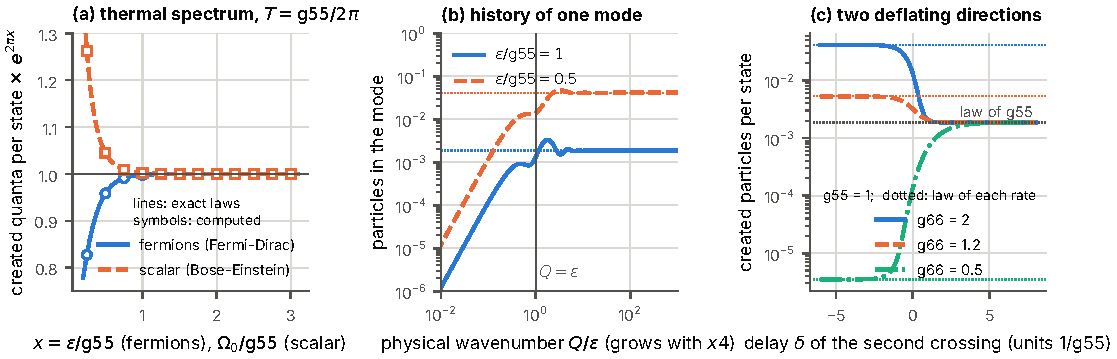
\includegraphics[width=\textwidth]{fig_creation}
\caption{\label{fig:creation}Creation of particles on the deflating $7{+}1$ spacetime. (a) Created
quanta per state, multiplied by $e^{2\pi\,\mathrm{ratio}}$, against the ratio of the energy to the
rate. Fermions follow the Fermi-Dirac law (\ref{eq:ncr}), the modes of the Vorton-Scalar the
Bose-Einstein law (\ref{eq:bose}), both at the temperature $\gff/2\pi$. Lines: the exact laws;
symbols: computed. (b) History of two modes, with $\Eperp/\gff=1$ and $0.5$: the number of particles
in the mode against the physical wavenumber $\kd/\Eperp$, which grows with the time. After the
crossing at $\kd=\Eperp$ the number settles at the value of Eq.~(\ref{eq:ncr}) (dotted). (c) Two
deflating directions, $\gff=1$ and $\gss=2$, $1.2$ or $0.5$: mean number of created particles per
state against the delay between the two crossings; the dotted lines are Eq.~(\ref{eq:ncr}) with each
of the two rates.}
\end{figure*}

The numerical solution of Eq.~(\ref{eq:h}) for all sixteen components confirms the law
(Fig.~\ref{fig:creation}). For $\Eperp/\gff$ between 0.25 and 3 the created number agrees with
Eq.~(\ref{eq:ncr}) to a relative deviation of at most $3.2\times10^{-6}$, while the numbers
themselves range from 0.17 to $6.5\times10^{-9}$; the eight internal states are created equally.
With three equal rates the result depends neither on the direction of the wavenumber nor on the
constants $\ct$. With unequal rates no exact solution is known. If the second physical wavenumber is
still below $e^{-3}\Eperp$ when the first reaches $\Eperp$, the mean created number is
Eq.~(\ref{eq:ncr}) with the rate of the coordinate that becomes energetic first, to within 1.2 per
cent. If two directions become energetic together, the eight internal states are created
\emph{unequally}, in the cases computed by up to a factor 110 between the most and the least
populated state, and the result is known only numerically.

\subsection{What the result means}

Each mode with $k_t\ne0$ is populated once, at its crossing. Its particles then gain energy without
bound, as $(\Eperp^{2}+\kd^{2})^{1/2}$, like the classical particle of Sec.~\ref{sec:geodesics}.
Modes with $k_t=0$ stay empty. Two remarks are in order.

First, the stress of the created particles must eventually change the metric. That reaction of the
fields on the metric has not been computed, and the results of this section hold for as long as it
can be neglected. For any rate of deflation that the bounds of Sec.~\ref{sec:cosmo} allow today the
temperature (\ref{eq:Tdefl}) is below $10^{-30}$~K, and nothing is created.

Second, the instantaneous energy of a quantum in a mode with $k_t\ne0$ is at least $|k_t|/b_t$,
which grows as $e^{\rt\,x4}$. A process with a given energy at its disposal can excite such a mode
only before the mode has crossed that energy. If the deflating coordinates are periodic, the
smallest wavenumber that differs from zero is fixed, and the sector of fields that do not depend on
$x5,x6,x7$ is separated from the rest by a gap that grows exponentially. This is the sense in which
the deflation supports the restriction to that sector, which the earlier paper assumed. If the
deflating coordinates are infinite, modes of arbitrarily small $k_t$ exist at every time, and the
restriction remains an assumption.

\subsection{The numerical method}

The equations of this section are linear, with coefficients that grow exponentially, and an
integrator with a fixed step fails on them. The program uses a commutator-free Magnus method of the
fourth order: over each step the solution is advanced by the product of two matrix exponentials of
linear combinations of the coefficient matrix at two Gauss points. Because the square of
$\hh$ is a multiple of the unit matrix at any one time, each exponential is evaluated in
closed form, and every step is exactly unitary. The length of a step is chosen so that
neither the phase accumulated in it nor the relative change of the coefficients exceeds a fixed
bound. The number of particles is read off by projection on the eigenstates of the
Hamiltonian corrected to the first order in the rate at which its direction changes, which removes
the leading spurious oscillation of the particle number at finite time. An independent program,
which uses an explicit Runge-Kutta method of the eighth order and the Bessel functions of another
library, reproduces Eq.~(\ref{eq:ncr}) to
$2.2\times10^{-5}$ \cite{DeflationRepo}.

\section{The Vorton-Scalar and the deflation clock}
\label{sec:clock}

\subsection{The model}

The earlier paper \cite{Flat1671} introduced a complex scalar field, the
\emph{Vorton-Scalar} $\PhiVS$, whose vacuum value gives the fermions their mass and whose exchange
binds two fermions into a pair. We restate the model on the deflating spacetime. It has three real,
positive constants: the self-coupling $\lamVS$ of the scalar, the constant $\vVS$ that fixes the
magnitude $\vVS/\sqrt2$ at which the potential of the scalar is lowest, and the Yukawa coupling
$\yVS$ of the scalar to the fermions. The chirality matrix is denoted by $\chi$, with
$\chi=i\,\gamma^{0}\gamma^{1}\cdots\gamma^{7}$,
and the chiral projectors are $P^{L,R}=\tfrac12(1\mp\chi)$.

On a curved spacetime a Lagrangian is multiplied by the volume factor $\Vd$, derivatives of spinors
become covariant derivatives, and the flat metric is replaced by the curved one.
For the Lagrangian of the earlier paper this gives
\begin{align}
\mathcal L_{\tg}^{\mathrm{VS}}=\Vd\,\Big[&\bar\psi\,i\gamma^{\mu}\nabla_\mu\psi
+g^{\mu\nu}\,\partial_\mu\PhiVS^{*}\,\partial_\nu\PhiVS\nonumber\\
&-\lamVS\Big(|\PhiVS|^{2}-\frac{\vVS^{2}}{2}\Big)^{2}\nonumber\\
&-\yVS\,\bar\psi\big(\PhiVS\,P^{R}+\PhiVS^{*}\,P^{L}\big)\psi\Big],
\label{eq:LVS}
\end{align}
with $\bar\psi=\psi^\dagger\beta$.
The Lagrangian has two phase symmetries, as on flat spacetime, because their transformations do not
involve the coordinates: the fermion number $U(1)_F$, $\psi\to e^{i\epsilon}\psi$, and the chiral
symmetry $\UVS$, $\psi\to e^{i\epsilon\chi}\psi$ with $\PhiVS\to e^{-2i\epsilon}\PhiVS$.

A constant field $\PhiVS=\vVS/\sqrt2$ with $\psi=0$ solves the field equations on the deflating
spacetime, because a constant has no derivatives: the vacuum value is the same at all times. It
breaks $\UVS$. Around it the Vorton-Scalar has two modes: the \emph{radial mode}, a real field of the
mass $m_s$, and the \emph{phase mode}, a real massless field, the Goldstone boson of the broken
symmetry. The fermions acquire the mass $m$. Both modes couple to the fermions with the same strength
$\gVS$, the radial mode to the scalar density $\bar\psi\psi$ and the phase mode to the pseudoscalar
density $\bar\psi\,i\chi\,\psi$:
\begin{equation}
\begin{aligned}
m&=\frac{\yVS\,\vVS}{\sqrt2},&\qquad m_s&=\sqrt{2\lamVS}\,\vVS,\\
\gVS&=\frac{m}{\vVS},&\qquad\aVS&=\frac{\gVS^{2}}{4\pi}.
\end{aligned}
\label{eq:masses}
\end{equation}

\subsection{Fields that do not depend on the extra coordinates}

As in the earlier paper, consider fields that do not depend on the four extra coordinates
$x0,x5,x6,x7$, and introduce the weighted fields
\begin{equation}
\hpsi=\sqrt{\Vd}\,\psi,\qquad\hat\Phi_{\mathrm{VS}}=\sqrt{\Vd}\,\PhiVS .
\end{equation}
Each term of Eq.~(\ref{eq:LVS}) is rewritten in turn. The kinetic term of the fermions is the flat
one for $\hpsi$ (Sec.~\ref{sec:dirac}). The Yukawa term contains one scalar and two fermion fields
and therefore the factor $\Vd\cdot\Vd^{-3/2}$. The potential becomes
$(\lamVS/\Vd)\,(|\hat\Phi_{\mathrm{VS}}|^{2}-\Vd\vVS^{2}/2)^{2}$. In the kinetic term of the scalar the
derivative along the time acts on the weight as well,
$\sqrt{\Vd}\,\partial_4\PhiVS=\partial_4\hat\Phi_{\mathrm{VS}}+\tfrac12\gsum\,\hat\Phi_{\mathrm{VS}}$,
which gives a term $\tfrac14\gsum^{2}|\hat\Phi_{\mathrm{VS}}|^{2}$ and a total derivative. The result
is the Lagrangian of the earlier paper for the weighted fields, with three replacements and one
additional term:
\begin{equation}
\begin{aligned}
&\yVS\to\frac{\yVS}{\sqrt{\Vd(x4)}},\qquad\lamVS\to\frac{\lamVS}{\Vd(x4)},\\
&\vVS\to\vVS\sqrt{\Vd(x4)},\qquad\text{and }+\frac{\gsum^{2}}{4}\,|\hat\Phi_{\mathrm{VS}}|^{2}.
\end{aligned}
\label{eq:couplings}
\end{equation}
The three replacements are those by which the earlier paper passed to the four-dimensional
description, where the volume of the extra coordinates was a constant. Here that volume is the
coordinate volume of a cell times $\Vd(x4)$, and it shrinks. The additional term lowers the square of
the mass of each mode of the scalar by $\gsum^{2}/4$ in the equation of the weighted field;
Section~\ref{sec:scalarmodes} shows what it does. From here on the couplings $\yVS$, $\lamVS$,
$\vVS$, $\gVS$ and $\aVS$ are those of the four-dimensional description at the time considered.

\subsection{The deflation clock}

Define the \emph{deflation clock}
\begin{equation}
\td=\gsum\,(x4-x4_{\mathrm{ref}}),
\label{eq:clock}
\end{equation}
the number of e-foldings by which the volume $\Vd$ has shrunk since a reference time
$x4_{\mathrm{ref}}$, which is chosen in each application. By Eq.~(\ref{eq:couplings}) every quantity
of the four-dimensional description is proportional to $e^{n\td}$ with a definite exponent $n$
(Table~\ref{tab:exponents}). Three observations organize what follows.

\begin{table*}
\caption{\label{tab:exponents}How the quantities of the four-dimensional description follow the
deflation clock: each is proportional to $e^{n\td}$. The last two rows hold under additional
assumptions, which Secs.~\ref{sec:cosmo} and \ref{sec:higgs} state and examine.}
\begin{ruledtabular}
\begin{tabular}{p{0.37\textwidth}p{0.47\textwidth}c}
quantity & meaning & exponent $n$ \\
\hline
$V_d$ & $b_5b_6b_7$: the factor $\sqrt{\lvert\det g\rvert}$ of the measure & $-1$ \\
$y_{\mathrm{VS}}$ of the four-dimensional description & Yukawa coupling of the weighted fields & $\tfrac12$ \\
$\lambda_{\mathrm{VS}}$ of the four-dimensional description & quartic coupling of the weighted Vorton-Scalar & $1$ \\
$v_{\mathrm{VS}}$ of the four-dimensional description & vacuum value of the weighted Vorton-Scalar & $-\tfrac12$ \\
$m$ & fermion mass $y_{\mathrm{VS}}v_{\mathrm{VS}}/\sqrt2$ & $0$ \\
$m_s$ & mass of the radial mode $\sqrt{2\lambda_{\mathrm{VS}}}\,v_{\mathrm{VS}}$ & $0$ \\
$g_{\mathrm{VS}}$ & coupling of the radial mode to the fermions, $m/v_{\mathrm{VS}}$ & $\tfrac12$ \\
$\alpha_{\mathrm{VS}}$ & $g_{\mathrm{VS}}^2/4\pi$ & $1$ \\
$G_{\mathrm{VS}}$ & constant of the Fermi type of the neutral-current interaction, $1/(\sqrt2\,v_{\mathrm{VS}}^2)$ & $1$ \\
$D_{\mathrm{VS}}$ & $\alpha_{\mathrm{VS}}\,m/m_s$: decides whether two fermions bind & $1$ \\
$C$ & $g_{\mathrm{VS}}^2m^2/m_s^2$: decides the state of matter & $1$ \\
vortex energy per length & proportional to $v_{\mathrm{VS}}^2$ (four-dimensional) & $-1$ \\
$G_{\mathrm{Fermi}}$ (Fermi constant of the weak interaction) if the vacuum value of the Vorton-Scalar sets the electroweak scale (assumption HV) & $1/(\sqrt2\,v_{\mathrm{VS}}^2)$, four-dimensional vacuum value & $1$ \\
$G_N$ (Newton's constant) if gravity is eight-dimensional (A2) & $G_8$ divided by the volume of $x5,x6,x7$ & $1$ \\
\end{tabular}
\end{ruledtabular}
\end{table*}

\emph{The masses do not change.} The fermion mass $m$ and the mass $m_s$ of the radial mode contain
the couplings in combinations from which the volume cancels. So do the Fermi momentum and the Fermi
energy of matter with a given number of particles per unit of ordinary volume.

\emph{The coupling grows.} The coupling $\gVS=m/\vVS$ grows as $e^{\td/2}$, because the
four-dimensional vacuum value falls. The strength of the attraction, $\aVS$, grows as $e^{\td}$: it
doubles every time the volume of the deflating coordinates halves.

\emph{The two numbers that decide the state of matter grow at the same rate.} These are
\begin{equation}
\DVS=\aVS\,\frac{m}{m_s},\qquad C=\frac{\gVS^{2}m^{2}}{m_s^{2}} .
\label{eq:DC}
\end{equation}
The first decides whether two fermions form a bound pair (Sec.~\ref{sec:pair}), the second whether
matter keeps its fermion mass (Sec.~\ref{sec:cjt}). Their ratio $C/\DVS=4\pi\,m/m_s$ is fixed.

A model of the earlier paper is specified by the masses and one coupling. On a deflating spacetime
it is specified by the masses and the value of the coupling \emph{at one time}; the deflation then
carries it through all larger couplings. The constants of the earlier paper become functions of the
time, and its thresholds are passed one after another (Fig.~\ref{fig:clock}).

\begin{figure*}
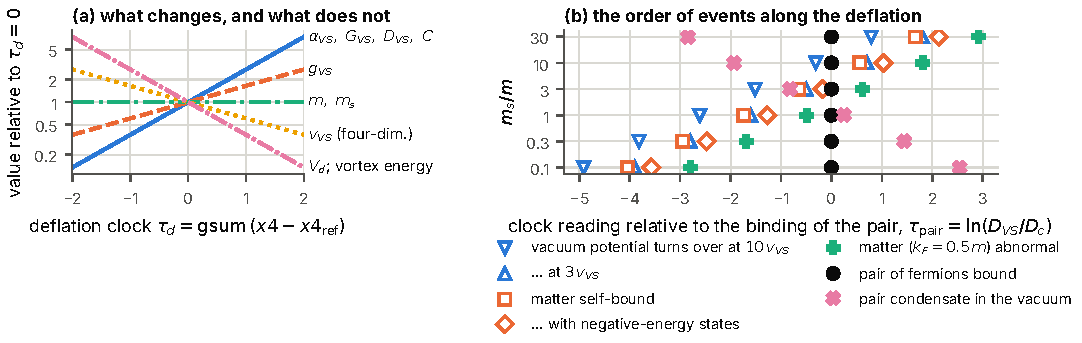
\includegraphics[width=0.9\textwidth]{fig_clock}
\caption{\label{fig:clock}The deflation clock. (a) How the quantities of the four-dimensional
description change with the clock $\td$ (logarithmic scale; values relative to $\td=0$). (b) The
order of events along the deflation for six ratios $m_s/m$: the clock reading of each event relative
to the moment at which two fermions form a bound pair (Table~\ref{tab:events}).}
\end{figure*}

\subsection{Modes of the Vorton-Scalar}
\label{sec:scalarmodes}

Let $\varphi_{\mathrm{bos}}$ stand for the radial mode or the phase mode, with the mass
$m_{\mathrm{bos}}=m_s$ or $m_{\mathrm{bos}}=0$. To first order in the field, a mode with a wavenumber
of the magnitude $k$ along the flat coordinates and the wavenumbers $k_t$ along the deflating ones
obeys
\begin{equation}
\begin{aligned}
&\frac{1}{\Vd}\,\partial_4\big(\Vd\,\partial_4\varphi_{\mathrm{bos}}\big)\\
&\quad+\Big(k^{2}+\sum_t\frac{k_t^{2}}{b_t^{2}}+m_{\mathrm{bos}}^{2}\Big)\varphi_{\mathrm{bos}}=0 .
\end{aligned}
\label{eq:scalar}
\end{equation}


\emph{Modes that do not depend on the deflating coordinates.} With $k_t=0$ the equation has constant
coefficients, and its solutions are the exponentials
\begin{equation}
\varphi_{\mathrm{bos}}\propto\exp\Big\{\Big[\frac{\gsum}{2}\pm\sqrt{\frac{\gsum^{2}}{4}-k^{2}-m_{\mathrm{bos}}^{2}}\,\Big]x4\Big\}.
\label{eq:exponents}
\end{equation}
If $k^{2}+m_{\mathrm{bos}}^{2}>\gsum^{2}/4$, the mode oscillates with the frequency
$\varpi_b=(k^{2}+m_{\mathrm{bos}}^{2}-\gsum^{2}/4)^{1/2}$, and its amplitude grows as
$e^{\gsum\,x4/2}$. The growth is that of the weight alone: the weighted field has a constant
amplitude, and the number of quanta in a cell of fixed coordinates is conserved while the cell
shrinks. Otherwise the mode does not oscillate. For the radial mode this never happens if
$m_s>\gsum/2$, which holds by many orders of magnitude for any rate that observation allows
(Sec.~\ref{sec:cosmo}). For the phase mode it happens at wavelengths longer than $4\pi/\gsum$. At
$k=0$ the two exponents of the phase mode are $0$ and $\gsum$: a constant phase, which costs nothing,
and a phase that advances at a rate proportional to $1/\Vd$, which is the conservation of the charge
of $\UVS$ in a shrinking volume. Neither is an instability of the vacuum. Figure~\ref{fig:scalar}
shows the exponents.

\begin{figure*}
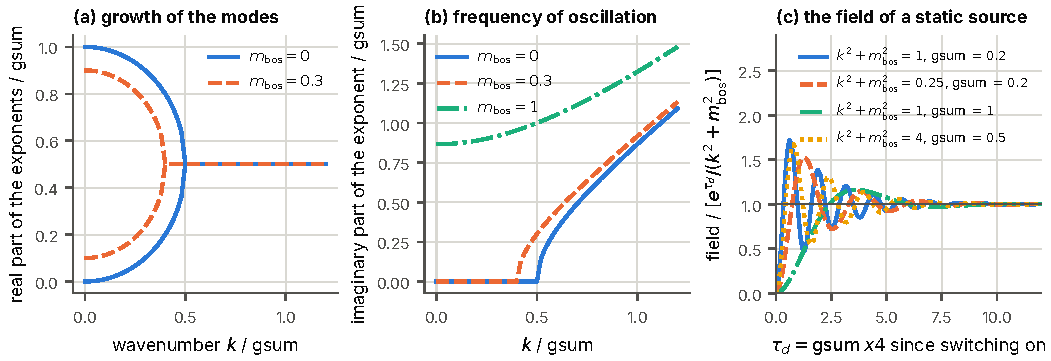
\includegraphics[width=\textwidth]{fig_scalar}
\caption{\label{fig:scalar}Modes of the Vorton-Scalar that do not depend on the deflating
coordinates. (a) Real parts of the two exponents of Eq.~(\ref{eq:exponents}) against the wavenumber,
for the phase mode and for a radial mode, in units of $\gsum$. (b) Their imaginary part, the
frequency of oscillation. (c) The field that a static source builds up from zero, divided by the form
$e^{\td}/(k^{2}+m_{\mathrm{bos}}^{2})$ that leads to Eq.~(\ref{eq:yukawa}).}
\end{figure*}

\emph{The potential between two fermions.} Two fermions at rest attract each other by exchanging the
radial mode. The density of a fixed number of fermions grows as $1/\Vd$, so that the radial mode
obeys Eq.~(\ref{eq:scalar}) with a source proportional to $e^{\gsum\,x4}$. The solution that follows
the source is $e^{\gsum\,x4}/(k^{2}+m_{\mathrm{bos}}^{2})$ times the source, as substitution shows:
the terms $\gsum^{2}-\gsum\cdot\gsum$ cancel, and the denominator contains the \emph{unshifted} mass.
The potential between two fermions at rest is therefore, at every moment, the Yukawa potential of
the earlier paper,
\begin{equation}
V_s(r)=-\aVS(x4)\,\frac{e^{-m_sr}}{r},
\label{eq:yukawa}
\end{equation}
with the range $1/m_s$ unchanged and the strength of the moment. The numerical solution from rest
approaches this form with a transient that decays as $e^{-\td/2}$ [Fig.~\ref{fig:scalar}(c)]; after
$\td=20$ the relative difference is below $4\times10^{-5}$ in the four cases computed.

\emph{Modes that depend on a deflating coordinate.} For $k_t\ne0$ the weighted field obeys
$\partial_4^{2}\hat\varphi_{\mathrm{bos}}+(\varpi_b^{2}+\kd^{2})\,\hat\varphi_{\mathrm{bos}}=0$
with the physical wavenumber $\kd$ of Eq.~(\ref{eq:kd}), and the scalar behaves as the fermion field
does.
The frequency grows without bound. When one rate governs, the solutions are Bessel functions of the
imaginary order $i\varpi_b/\rt$ and of the argument $\ud$, and a mode that starts empty ends with
\begin{equation}
\ncr=\frac{1}{e^{2\pi\varpi_b/\rt}-1}
\label{eq:bose}
\end{equation}
quanta: the Bose-Einstein distribution at the same temperature $\Tdefl$ as for the fermions. The
program confirms Eq.~(\ref{eq:bose}) in 36 cases to a relative deviation of $1.9\times10^{-5}$
(Fig.~\ref{fig:creation}).

\section{Pairing and the gap along the clock}
\label{sec:gap}

\subsection{The pair channels}

A pair of fermions is created by an operator $\psi^{T}X\psi$ with a $16\times16$ matrix $X$; the
choice of $X$ is the \emph{channel} of the pair. The earlier paper classified the channels and
computed, for each, the \emph{exchange amplitudes} $F_S$ and $F_P$ of the radial mode and of the
phase mode: the matrix elements of the exchange of one boson between two fermions of opposite
momenta in the internal state of the channel. It found that the radial mode attracts in every
channel, and that the phase mode attracts in the four \emph{vector pairs along the extra axes},
\begin{equation}
\psi^{T}\Cm\gamma^{a}\psi,\qquad a\in\{0,5,6,7\},
\label{eq:pairs}
\end{equation}
and repels in their partners that are built with two Dirac matrices. Here
$\Cm=\gamma^{4}\gamma^{0}\gamma^{1}\cdots\gamma^{7}$
is the matrix that turns each Dirac matrix into minus its transpose, and the index $a$ labels the
four extra axes. The pair along the hidden axis, $a=0$, has spin 0 in ordinary spacetime; it is the
\emph{hidden-axis singlet} of hypothesis H1.

The amplitudes are computed from the Dirac matrices of the frame, which the deflation does not
change, and each is proportional to the square of the coupling. For fields that do not depend on
$x5,x6,x7$ the amplitude of a channel at the time $x4$ is therefore
\begin{equation}
\begin{aligned}
F_{S,P}(x4)={}&\gVS(x4)^{2}\\
&\times\big(F_{S,P}\text{ of the flat spacetime at }\gVS=1\big).
\end{aligned}
\label{eq:amplitudes}
\end{equation}
The program computes the amplitudes of the 15 representative channels of the earlier paper again
from the matrices of the deflating spacetime, at three momenta and 13 scattering angles; the numbers
agree with those of the earlier paper to every digit recorded there,
and the amplitudes of the hidden-axis channel reproduce its closed forms to $1.1\times10^{-15}$. The
conclusion of the earlier paper about the channels therefore stands at every moment
(Fig.~\ref{fig:kernels}): the most attractive channel is the vector pair along an extra axis.

\begin{figure*}
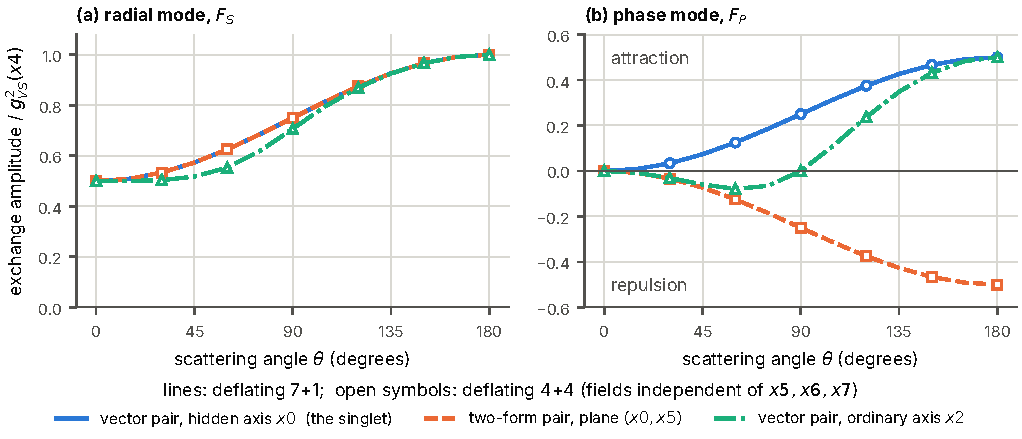
\includegraphics[width=0.84\textwidth]{fig_kernels}
\caption{\label{fig:kernels}Exchange amplitudes in three pair channels, divided by the square of the
coupling of the moment, against the scattering angle, for momenta of the magnitude $m$ in the plane
of $x1$ and $x2$. Lines: deflating $7{+}1$ spacetime; open symbols: deflating $4{+}4$ spacetime. (a) The
radial mode attracts in all three channels. (b) The phase mode attracts in the vector pair along the
hidden axis and repels in its partner built with two Dirac matrices. The amplitudes are those of flat
spacetime: the deflation changes their overall strength and nothing else.}
\end{figure*}

\subsection{The gap grows much faster than the coupling}

In matter of a given density the attraction opens a gap $\Delta_F$ at the Fermi momentum $\kF$: the
energy that it costs to break a pair. The gap equation of the earlier paper, which generalizes that
of Bardeen, Cooper and Schrieffer \cite{BCS1957}, holds at each moment with the couplings of that
moment. Its solution as a function of the clock is the \emph{adiabatic history} of the paired state:
the state that matter would have if it were always in equilibrium. (Section~\ref{sec:quench}
examines when it can be.) The strength of the pairing is measured by the dimensionless number
$\lambda=N(0)\,W(\kF,\kF)$, the density of states at the Fermi surface times the kernel of the gap
equation there; in the vector channel it is the sum $\lambda_S+\lambda_P$ of the contributions of the
two modes. Since the kernel is proportional to $\gVS^{2}$,
\begin{equation}
\lambda\ \propto\ e^{\td}.
\end{equation}

The program solves the gap equation at 34 moments for each of four sets of the mass $m_s$ and the
Fermi momentum (Table~\ref{tab:gap}, Fig.~\ref{fig:gap}). There are three results.

\begin{table*}
\caption{\label{tab:gap}The gap along the deflation clock for two of the four sets computed. $\gVS$
and $\lambda$: coupling and pairing strength of the moment. $\EF$: Fermi kinetic energy. $T_c$:
critical temperature. Rate of growth: $d\ln\Delta_F/d\td$; the last column, its product with
$\lambda$, is given where the gap is between $10^{-6}$ and $0.02$ of $\EF$.}
\begin{ruledtabular}
\begin{tabular}{cccccccc}
$m_s/m$, $\kF/m$ & $\td$ & $\gVS$ & $\lambda$ & $\Delta_F/\EF$ & $T_c/\Delta_F$ & rate of growth & $\lambda\,\times$ rate \\
\hline
0.10, 0.50 & $-0.63$ & 0.730 & 0.062 & $1.17\times10^{-7}$ & 0.567 & --- & --- \\
0.10, 0.50 & $-0.13$ & 0.939 & 0.102 & $7.40\times10^{-5}$ & 0.567 & 9.88 & 1.01 \\
0.10, 0.50 & 0.38 & 1.208 & 0.169 & $3.70\times10^{-3}$ & 0.567 & 6.01 & 1.01 \\
0.10, 0.50 & 0.88 & 1.554 & 0.279 & 0.0407 & 0.565 & 3.74 & --- \\
0.10, 0.50 & 1.39 & 2.000 & 0.463 & 0.189 & 0.555 & 2.50 & --- \\
0.10, 0.50 & 1.89 & 2.573 & 0.766 & 0.563 & 0.528 & 1.96 & --- \\
0.10, 0.50 & 2.39 & 3.311 & 1.268 & 1.49 & 0.480 & 1.96 & --- \\
1.0, 0.50 & 0.88 & 1.554 & 0.056 & $1.02\times10^{-7}$ & 0.567 & --- & --- \\
1.0, 0.50 & 1.13 & 1.763 & 0.072 & $5.62\times10^{-6}$ & 0.567 & 14.02 & 1.01 \\
1.0, 0.50 & 1.39 & 2.000 & 0.092 & $1.27\times10^{-4}$ & 0.567 & 10.93 & 1.01 \\
1.0, 0.50 & 1.64 & 2.269 & 0.119 & $1.45\times10^{-3}$ & 0.567 & 8.54 & 1.02 \\
1.0, 0.50 & 1.89 & 2.573 & 0.153 & $9.76\times10^{-3}$ & 0.567 & 6.71 & 1.03 \\
1.0, 0.50 & 2.14 & 2.919 & 0.197 & 0.0439 & 0.566 & 5.33 & --- \\
1.0, 0.50 & 2.39 & 3.311 & 0.253 & 0.147 & 0.563 & 4.37 & --- \\
\end{tabular}
\end{ruledtabular}
\end{table*}

\emph{The order of the channels does not change.} At every moment the gap of the vector channel is
at least as large as the gap that the radial mode alone would give, and that at least as large as
the gap of the channel in which the phase mode repels. The gap never decreases.

\emph{The critical temperature follows the gap.} Wherever the gap is below 5 per cent of the Fermi
kinetic energy $\EF$, the critical temperature is $T_c=0.567\,\Delta_F$, the ratio of weak coupling,
to within 0.002.

\emph{The law of growth.} In weak coupling the gap is proportional to $e^{-1/\lambda}$. With
$\lambda\propto e^{\td}$,
\begin{equation}
\frac{d\ln\Delta_F}{d\td}=\frac{1}{\lambda}.
\label{eq:growth}
\end{equation}
In the computed histories the product $\lambda\,d\ln\Delta_F/d\td$ lies between 1.00 and 1.03
wherever the gap is between $10^{-6}$ and $0.02$ of $\EF$.

Equation (\ref{eq:growth}) is the central quantitative statement about the superfluid on a deflating
spacetime. While the coupling grows by one e-folding, the gap of a weakly paired state with
$\lambda=0.1$ grows by ten e-foldings, a factor of twenty thousand. A paired state that is
unobservably weak at one time is strong a few e-foldings of the volume later.

\begin{figure*}
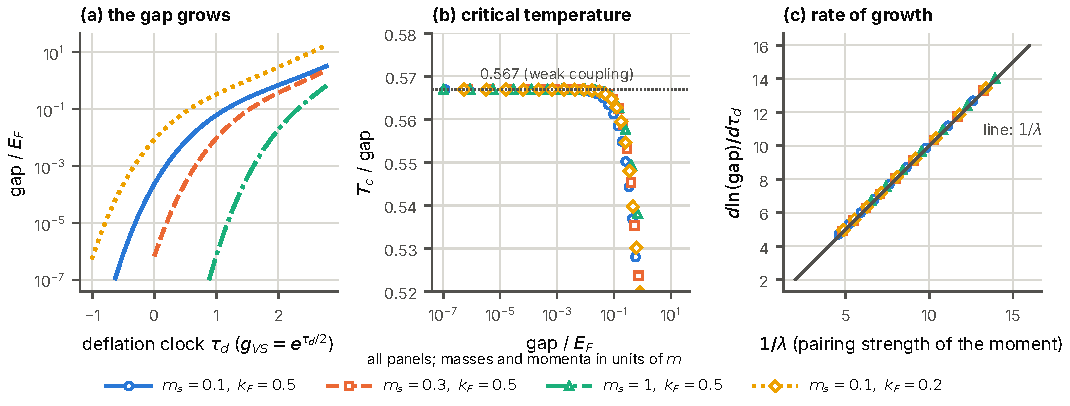
\includegraphics[width=\textwidth]{fig_gap_history}
\caption{\label{fig:gap}The gap along the deflation clock, for four sets of the mass of the radial
mode and of the Fermi momentum (in units of $m$). (a) The gap of the vector channel in units of the
Fermi kinetic energy. (b) The ratio of the critical temperature to the gap. (c) The rate of growth of
the gap against $1/\lambda$; the line is Eq.~(\ref{eq:growth}).}
\end{figure*}

\section{The bound pair and the order of events}
\label{sec:pair}

\subsection{The moment of binding}

Two fermions in the Yukawa potential (\ref{eq:yukawa}) form a bound state if and only if the number
$\DVS$ of Eq.~(\ref{eq:DC}) exceeds a critical value, $D_c=1.67981$. On a deflating spacetime
$\DVS\propto e^{\td}$, so that the pair becomes bound at a definite time. Measure the clock from that
moment:
\begin{equation}
\tpair=\ln\frac{\DVS}{D_c}=\gsum\,\big(x4-x4_{\mathrm{binding}}\big).
\label{eq:tpair}
\end{equation}
Table~\ref{tab:dimer} and Fig.~\ref{fig:binding} show the scattering length $a_{\mathrm{sc}}$ of two
fermions and the binding energy $E_b$ of the pair as the clock passes the binding.

\begin{table}
\caption{\label{tab:dimer}Two fermions as the clock passes the moment of binding: the scattering
length in units of $1/m_s$, the number of bound states, and the binding energy in units of
$m_s^{2}/m$.}
\begin{ruledtabular}
\begin{tabular}{ccccc}
$\tpair$ & $\DVS$ & $a_{\mathrm{sc}}\,m_s$ & bound states & $E_b\,m/m_s^{2}$ \\
\hline
$-0.105$ & 1.5118 & $-12.50$ & 0 & 0 \\
$-0.095$ & 1.5279 & $-13.93$ & 0 & 0 \\
$-0.010$ & 1.6630 & $-134.0$ & 0 & 0 \\
0.010 & 1.6966 & 135.9 & 1 & $5.50\times10^{-5}$ \\
0.486 & 2.7314 & 2.698 & 1 & 0.232 \\
0.994 & 4.5409 & $-0.1288$ & 1 & 1.82 \\
\end{tabular}
\end{ruledtabular}
\end{table}

\emph{The scattering length.} Just before the binding the scattering length is large and negative,
just after it large and positive: $-134.0/m_s$ at $0.99\,D_c$ and $+135.9/m_s$ at $1.01\,D_c$. At the
moment of binding it is infinite: the two fermions are at a scattering resonance. \emph{Every pair
of fermions of the model passes through this resonance once, at the same time.}
Section~\ref{sec:cosmo} examines what that means if the fermions are the dark matter.

\emph{The binding energy.} Just after the binding the binding energy starts quadratically,
\begin{equation}
E_b\ \propto\ \big(e^{\tpair}-1\big)^{2}\,\frac{m_s^{2}}{m},
\label{eq:Eb}
\end{equation}
with the fitted exponent 2.01 between 2 and 8 per cent above $D_c$. Because $E_b$ vanishes at the
threshold, the time $1/E_b$ that the pair needs to adjust is infinite there. However slow the
deflation is, the pair cannot follow it adiabatically at first.

\emph{The same threshold from the gap equation.} In vacuum the linearized gap equation is the
equation of a bound state of two fermions, with a relativistic kernel. It reaches the eigenvalue 1 at
$\DVS=1.7347$, $1.6902$ and $1.6810$ for $m_s/m=0.3$, $0.1$ and $0.03$, approaching the value
$D_c$ of the Schr\"odinger equation as the radial mode becomes light and the binding
non-relativistic.

\begin{figure*}
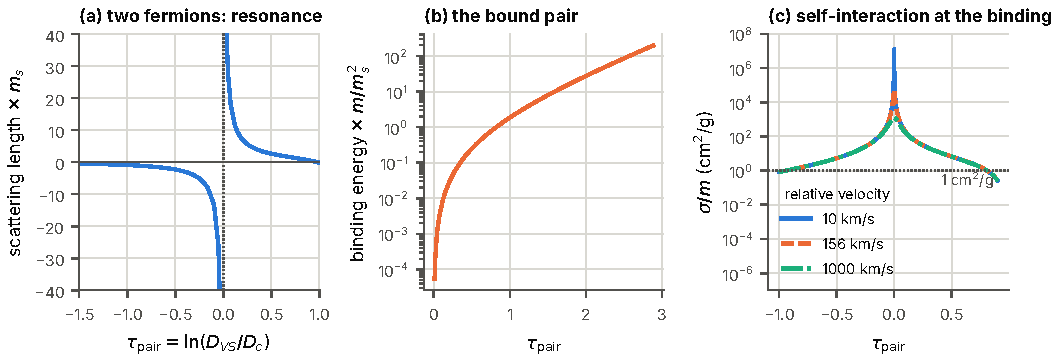
\includegraphics[width=\textwidth]{fig_binding}
\caption{\label{fig:binding}The bound pair along the clock. (a) Scattering length of two fermions in
units of $1/m_s$ against $\tpair$: the resonance at the moment of binding. (b) Binding energy of the
pair. (c) Cross-section per mass of two fermions at three relative velocities while the clock passes
the binding, for the example particle of Sec.~\ref{sec:dm}.}
\end{figure*}

\subsection{The order of events}

The other thresholds of the earlier paper are thresholds in the number $C$ of Eq.~(\ref{eq:DC}),
which grows at the same rate as $\DVS$. Because $C/\DVS=4\pi m/m_s$ is fixed, the order in which the
events happen depends on the ratio $m_s/m$ alone. Table~\ref{tab:events} gives the clock reading
$\tpair$ of each event; a negative number means that the event precedes the binding of the pair. The
events other than the binding are derived in Sec.~\ref{sec:cjt}.

\begin{table*}
\caption{\label{tab:events}The order of events along the deflation: the clock reading $\tpair$ of
each event, relative to the moment at which two fermions form a bound pair, for six ratios of the
mass $m_s$ of the radial mode to the fermion mass $m$.}
\begin{ruledtabular}
\begin{tabular}{p{0.42\textwidth}lcccccc}
event & threshold & $0.1$ & $0.3$ & $1$ & $3$ & $10$ & $30$ \\
\hline
the one-loop potential of the Vorton-Scalar falls below its vacuum value at the field $10\,v_{\mathrm{VS}}$ & $C=1.5477$ & $-4.92$ & $-3.82$ & $-2.61$ & $-1.51$ & $-0.31$ & 0.79 \\
matter is self-bound (Fermi sea only) & $C=3.7011$ & $-4.04$ & $-2.94$ & $-1.74$ & $-0.64$ & 0.56 & 1.66 \\
the one-loop potential falls below its vacuum value at the field $3\,v_{\mathrm{VS}}$ & $C=4.2694$ & $-3.90$ & $-2.80$ & $-1.60$ & $-0.50$ & 0.70 & 1.80 \\
matter is self-bound (with the negative-energy states) & $C=5.9218$ & $-3.57$ & $-2.48$ & $-1.27$ & $-0.17$ & 1.03 & 2.13 \\
matter of Fermi momentum $0.5\,m$ becomes abnormal (massless fermions) & $C=12.9713$ & $-2.79$ & $-1.69$ & $-0.49$ & 0.61 & 1.82 & 2.91 \\
\textbf{two fermions form a bound pair} & $D_{\mathrm{VS}}=1.6798$ & 0.00 & 0.00 & 0.00 & 0.00 & 0.00 & 0.00 \\
pair condensate in the vacuum (ladder equation, cutoff $100\,m$) & $\alpha_{\mathrm{VS}}=2.13$ to $2.93$ & 2.54 & 1.44 & 0.25 & $-0.82$ & $-1.93$ & $-2.84$ \\
\end{tabular}
\end{ruledtabular}
\end{table*}

For a \emph{light radial mode}, $m_s/m\le3$ in the table, the pair becomes bound only \emph{after}
the one-loop potential of the Vorton-Scalar has fallen below its vacuum value at a field of three
times the vacuum value: the deflation endangers the vacuum of the model before it binds the pair. The
condition for the opposite order is $4\pi D_c\,m/m_s<4.27$, that is, $m_s/m>4.9$. For a \emph{heavy
radial mode}, $m_s/m=10$ or $30$, the pair becomes bound first, and matter becomes self-bound and
loses its fermion mass later. Nothing in the model decides between the two orders; the table states
what follows from each.

\section{Can the paired state follow the deflation?}
\label{sec:quench}

\subsection{The question, and the parameter that decides it}

Section~\ref{sec:gap} gave the gap that the paired state would have in equilibrium at each moment.
But a state can change at most at the rate of its own energy scale, which for a paired state is the
gap. By Eq.~(\ref{eq:growth}) the equilibrium gap, written $\Deq$ in this section, changes at the
rate $\gsum/\lambda$. The paired state can follow only if that rate is small compared with the gap
itself:
\begin{equation}
\Xid=\frac{\gsum}{\lambda\,\Deq}\ \ll\ 1 .
\label{eq:Xi}
\end{equation}
Early in the deflation the gap is exponentially small, and the condition fails however small the
rate is. A system that is carried through a change faster than it can respond falls out of
equilibrium, as in the formation of defects at a phase transition \cite{Kibble1976,Zurek1985}. The
question is what the paired state does then, and when it catches up.

\subsection{The model}

The question is answered with the standard reduced model of a superfluid, whose dynamics without
collisions is known in detail \cite{BarankovLevitovSpivak2004}. Pairs of states of opposite momenta,
with the single-particle energy $\xi_k$ measured from the Fermi energy, fill a shell
$-\Esh<\xi_k<\Esh$ with a constant density of states, and all attract one another with the
dimensionless strength $\lambda$. In the mean-field approximation each pair of states is described by
its pair correlation $\kappa$, a complex number, and its occupation $n_k$; the order parameter is
$\Delta=\lambda\int\kappa\,d\xi_k$. The equations of motion are
\begin{align}
\frac{d\kappa}{dx4}&=-i\,\big[2\,\xi_k\,\kappa-\Delta\,(1-2n_k)\big],\nonumber\\
\frac{dn_k}{dx4}&=2\,\mathrm{Im}\big(\Delta^{*}\kappa\big).
\label{eq:bloch}
\end{align}
They conserve $|2\kappa|^{2}+(1-2n_k)^{2}=1$ for every pair of states. In equilibrium
$\kappa=\Delta/2E_k$ and $n_k=\tfrac12(1-\xi_k/E_k)$ with the quasi-particle energy
$E_k=(\xi_k^{2}+\Delta^{2})^{1/2}$, and the gap equation gives
\begin{equation}
\Deq(\lambda)=\frac{\Esh}{\sinh(1/\lambda)}\ \approx\ 2\,\Esh\,e^{-1/\lambda}\quad(\lambda\ll1).
\end{equation}
The model keeps what matters for the question, a gap that depends exponentially on a coupling that
grows exponentially, and omits the dependence of the gap on the momentum; $\Esh$ stands for the
range of energies over which the attraction acts. The program starts the model in equilibrium at
$\lambda=0.15$, lets the coupling grow as $\lambda=0.15\,e^{\td}$ up to $\lambda=0.5$, and integrates
Eqs.~(\ref{eq:bloch}) for 2000 energies. Doubling the number of energies and halving the step
changes no digit of the results quoted. Besides $|\Delta|$ the program records the density $\nex$ of
\emph{broken pairs}: the number of pairs of states, per unit of $\Esh$ times the density of states,
that are not in the ground state that belongs to the order parameter of the moment. In equilibrium
it is zero.

\subsection{Results}

\begin{table*}
\caption{\label{tab:quench}The paired state while the pairing strength grows from 0.15 to 0.5, for
seven rates of deflation: the parameter $\Xid$ at the start; the smallest ratio of the order
parameter to the equilibrium gap of the moment; the clock reading at which the order parameter has
returned to within 10 per cent of the equilibrium gap, and $\Xid$ at that moment; the ratio at the
end; and the density of broken pairs at the end.}
\begin{ruledtabular}
\begin{tabular}{ccccccc}
$\gsum/\Esh$ & $\Xid$ at the start & smallest $|\Delta|/\Deq$ & $\td$ of the catch-up & $\Xid$ there & final $|\Delta|/\Deq$ & $\nex$ at the end \\
\hline
$1\times10^{-4}$ & 0.262 & 0.958 & 0.020 & 0.23 & 1.0000 & $6.0\times10^{-6}$ \\
$3\times10^{-4}$ & 0.786 & 0.890 & 0.069 & 0.47 & 0.9998 & $5.1\times10^{-5}$ \\
$1\times10^{-3}$ & 2.62 & 0.737 & 0.234 & 0.52 & 0.9980 & $4.4\times10^{-4}$ \\
$3\times10^{-3}$ & 7.86 & 0.539 & 0.454 & 0.44 & 0.9886 & $2.4\times10^{-3}$ \\
0.01 & 26.2 & 0.328 & 0.780 & 0.32 & 0.9347 & 0.012 \\
0.03 & 78.6 & 0.189 & 1.172 & 0.24 & 0.8076 & 0.041 \\
0.1 & 262 & 0.098 & --- & --- & 0.1189 & 0.022 \\
\end{tabular}
\end{ruledtabular}
\end{table*}

Table~\ref{tab:quench} and Fig.~\ref{fig:quench} show three results.

\emph{The faster the deflation, the further the order parameter falls behind.} For a rate of
$10^{-4}\,\Esh$ the order parameter drops to 0.958 of the equilibrium gap of the moment before it
recovers; for $10^{-1}\,\Esh$ it drops to 0.098.

\emph{The state catches up when $\Xid$ has fallen to a value between 0.23 and 0.52.} In six of the
seven runs the order parameter returns to within 10 per cent of the equilibrium gap at such a value.
In the fastest run it has not caught up when the coupling reaches 0.5. This confirms the estimate
(\ref{eq:Xi}) and fixes the number that ``small'' means.

\emph{The lag leaves broken pairs behind.} Their density at the end grows with the rate, from
$6.0\times10^{-6}$ to $4.1\times10^{-2}$ in the six slower runs. They are excitations of the
superfluid that the deflation itself has made; in a system without dissipation they remain.

Because $\Deq$ grows as $e^{-1/\lambda}$ while $\lambda$ grows only as $e^{\td}$, the parameter
$\Xid$ falls steeply with time. For any rate there is a moment at which $\Xid$ passes through the
window of the second result. Before it the paired state is out of equilibrium, with an order
parameter below the equilibrium value; after it the adiabatic history of Sec.~\ref{sec:gap}
applies. The slower the deflation, the earlier that moment and the smaller the gap at which it
happens: it is the moment at which the equilibrium gap has grown to between two and four times
$\gsum/\lambda$.

\begin{figure*}
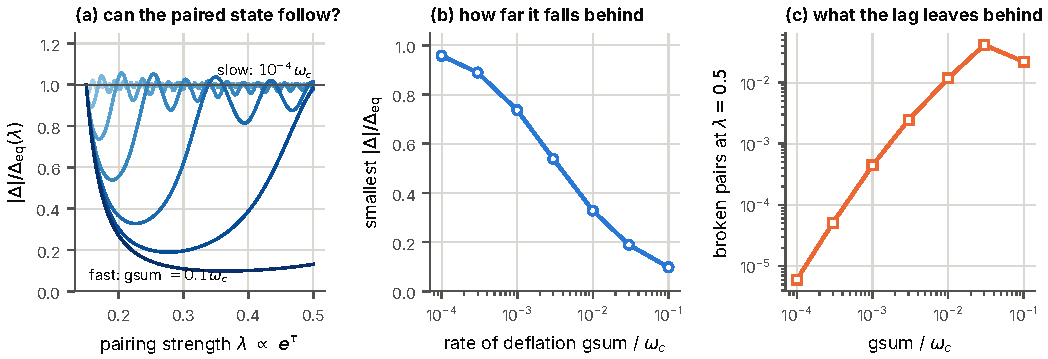
\includegraphics[width=\textwidth]{fig_quench}
\caption{\label{fig:quench}The paired state while the coupling grows. (a) The order parameter
divided by the equilibrium gap of the moment, against the pairing strength, for seven rates of
deflation. (b) The smallest value of that ratio against the rate. (c) The density of broken pairs at
the end of the run against the rate.}
\end{figure*}

\section{The effective action along the clock}
\label{sec:cjt}

\subsection{The method, and why it carries over}

The earlier paper derived its results on the paired state, on matter, on temperature and on the
vacuum from the effective action for composite operators of Cornwall, Jackiw and Tomboulis (CJT)
\cite{CJT1974}: a functional of the expectation value $\phi$ of the Vorton-Scalar and of the full
propagators, whose two-particle-irreducible part is truncated at two loops. Its stationarity
conditions are the equation for the fermion mass in matter and the gap equation. On the deflating
spacetime, and for fields that do not depend on the extra coordinates, nothing in this construction
changes, for two reasons established above. The weighted fermion field obeys the flat equations, so
that its propagator is the flat one. And the interaction between the fermions is, at each moment,
the exchange of the two modes of the scalar with the coupling of that moment and with the unshifted
range (Sec.~\ref{sec:scalarmodes}).

The one new term, the shift $-\gsum^{2}/4$ of the squares of the boson masses in
Eq.~(\ref{eq:couplings}), is smaller than every other scale of the calculation by the square of the
ratio of the rate of deflation to a particle mass. For the largest rate that observation allows
(Sec.~\ref{sec:cosmo}) and a mass of 1~keV that ratio is below $10^{-36}$. The term is neglected in
this section; this is the only approximation made here beyond those of the earlier paper. The test
of the truncation on a solvable model in zero dimensions, which does not involve the spacetime, was
executed again: the two-loop truncation has a solution for every coupling from 0.01 to 30 and stays
within 10.7 per cent of the exact propagator.

Every result of this section is a statement about a \emph{sequence of equilibrium states}. Whether a
system can follow the sequence was examined, for the paired state, in Sec.~\ref{sec:quench}.

\subsection{The paired state}

The CJT potential $V[\Delta]$ of the paired state is the effective action per unit volume, measured
from the unpaired state, as a functional of the gap function $\Delta(k)$. The program evaluates it at
13 moments, for two choices of the mass $m_s$ at the Fermi momentum $\kF=0.5\,m$, in the vector
channel (Table~\ref{tab:cjt}, Fig.~\ref{fig:cjt}).

\begin{table*}
\caption{\label{tab:cjt}The paired state along the clock from the CJT potential, for $\kF=0.5\,m$.
$\lambda$: pairing strength. $V$: the potential at the solution, the condensation energy. Ratio: $V$
divided by its weak-coupling value $-\nu N(0)\Delta_F^{2}/4$, with $\nu=8$ internal states and the
density of states $N(0)$. Curvature: the smallest eigenvalue of the matrix of second derivatives of
the potential. Size: the coherence length of the pair in units of $1/\kF$.}
\begin{ruledtabular}
\begin{tabular}{cccccccccc}
$m_s/m$, $\kF/m$ & $\td$ & $\gVS$ & $\lambda$ & $\Delta_F/m$ & $V/m^{4}$ & ratio & curvature & $T_c/\Delta_F$ & size $\times\kF$ \\
\hline
0.30, 0.50 & 0.00 & 1.80 & 0.216 & $2.81\times10^{-3}$ & $-4.46\times10^{-7}$ & 1.000 & 0.21 & 0.567 & 25.4 \\
0.30, 0.50 & 0.21 & 2.00 & 0.266 & $6.89\times10^{-3}$ & $-2.68\times10^{-6}$ & 0.998 & 0.26 & 0.566 & 10.3 \\
0.30, 0.50 & 0.40 & 2.20 & 0.322 & 0.0135 & $-1.03\times10^{-5}$ & 0.992 & 0.30 & 0.564 & 5.3 \\
0.30, 0.50 & 0.58 & 2.40 & 0.383 & 0.0230 & $-2.93\times10^{-5}$ & 0.981 & 0.34 & 0.559 & 3.1 \\
0.30, 0.50 & 0.74 & 2.60 & 0.450 & 0.0354 & $-6.81\times10^{-5}$ & 0.961 & 0.37 & 0.552 & 2.0 \\
0.30, 0.50 & 0.88 & 2.80 & 0.522 & 0.0511 & $-1.38\times10^{-4}$ & 0.932 & 0.38 & 0.542 & 1.4 \\
0.30, 0.50 & 1.02 & 3.00 & 0.599 & 0.0707 & $-2.53\times10^{-4}$ & 0.895 & 0.38 & 0.530 & 1.0 \\
1.0, 0.50 & 0.00 & 2.40 & 0.133 & $4.25\times10^{-4}$ & $-1.02\times10^{-8}$ & 1.000 & 0.13 & 0.567 & 167.6 \\
1.0, 0.50 & 0.16 & 2.60 & 0.156 & $1.32\times10^{-3}$ & $-9.88\times10^{-8}$ & 1.000 & 0.15 & 0.567 & 53.9 \\
1.0, 0.50 & 0.31 & 2.80 & 0.181 & $3.28\times10^{-3}$ & $-6.08\times10^{-7}$ & 0.999 & 0.17 & 0.567 & 21.7 \\
1.0, 0.50 & 0.45 & 3.00 & 0.208 & $6.89\times10^{-3}$ & $-2.68\times10^{-6}$ & 0.998 & 0.19 & 0.566 & 10.3 \\
1.0, 0.50 & 0.58 & 3.20 & 0.237 & 0.0128 & $-9.25\times10^{-6}$ & 0.994 & 0.21 & 0.564 & 5.6 \\
1.0, 0.50 & 0.70 & 3.40 & 0.267 & 0.0218 & $-2.65\times10^{-5}$ & 0.987 & 0.23 & 0.561 & 3.3 \\
\end{tabular}
\end{ruledtabular}
\end{table*}

\emph{The solution of the gap equation is a minimum at every moment.} Newton's method applied to the
potential converges to the gap function that the iteration of the gap equation finds, to
$7.7\times10^{-12}$, and the smallest eigenvalue of the second variation is positive throughout. The
temperature at which the second variation at $\Delta=0$ loses its positivity equals the temperature
at which the linearized gap equation has the eigenvalue 1, to $2.6\times10^{-12}$: two routes to the
critical temperature agree.

\emph{The condensation energy deepens.} It is within 15 per cent of the weak-coupling value wherever
the gap is below $0.1\,\EF$, and in weak coupling its logarithmic slope along the clock is twice that
of the gap, by Eq.~(\ref{eq:growth}):
\begin{equation}
\frac{d\ln|V|}{d\td}=\frac{2}{\lambda}.
\end{equation}

\emph{The pairs shrink.} The coherence length of the first set falls from 25 to 1.0 in units of
$1/\kF$. At its last five moments the gap exceeds $0.1\,\EF$, and at the last the pair is as small
as the distance between the particles. \emph{The deflation carries the paired state from overlapping
pairs toward bound pairs.} On flat spacetime this crossover \cite{NozieresSchmittRink1985,Leggett1975}
is reached by choosing a larger coupling; here it is reached by waiting.

\emph{The universal ratios hold while the coupling is weak.} While the critical temperature rises by
a factor of sixteen, from $6.3\times10^{-3}$ to $0.10$ of the Fermi energy, the ratio of the gap at
zero temperature to the critical temperature stays within 0.019 of the weak-coupling value 1.7639,
and the relative jump of the heat capacity at $T_c$ within 0.048 of 1.4261. The coefficients of the
Ginzburg-Landau energy agree with their weak-coupling formulas to 1.0 per cent while $T_c$ is below
$0.05\,\EF$ and differ by up to 7.9 per cent at $T_c=0.10\,\EF$. The coherence length of the
Ginzburg-Landau energy, $0.1333\,v_F/T_c$ in weak coupling with the Fermi velocity $v_F$, shrinks
from 80 to 5.1 in units of $1/m$: the cores of the vortices of the superfluid shrink as the
deflation proceeds.

\begin{figure*}
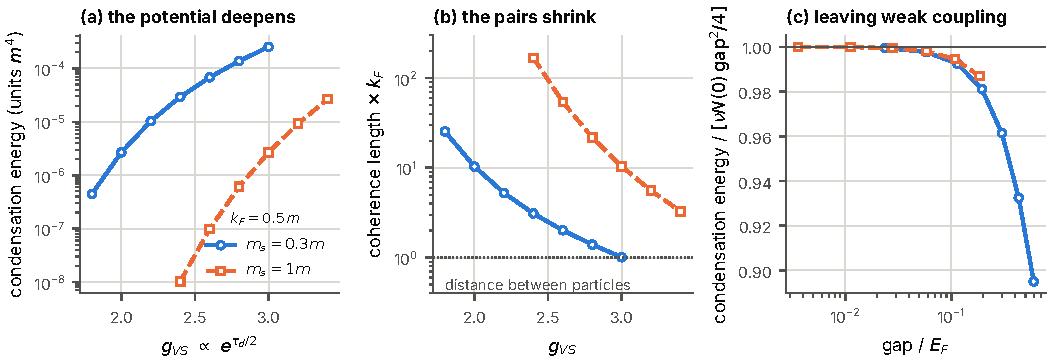
\includegraphics[width=\textwidth]{fig_cjt_history}
\caption{\label{fig:cjt}The paired state along the clock, from the CJT potential, for the two sets of
Table~\ref{tab:cjt}. (a) The condensation energy against the coupling of the moment. (b) The
coherence length of the pair in units of $1/\kF$. (c) The condensation energy divided by its
weak-coupling value, against the gap in units of the Fermi kinetic energy: the departure from weak
coupling.}
\end{figure*}

\subsection{Matter}

\emph{Matter of fixed density loses its fermion mass.} In matter the expectation value of the
Vorton-Scalar is reduced by the scalar density of the fermions, and with it the fermion mass in the
matter, $m^{*}$. The earlier paper showed that the reduction depends on the density and on the
single number $C$, and that above a critical value of $C$ the mass vanishes: the matter is then in
the \emph{abnormal} state of Lee and Wick \cite{LeeWick1974}, a gas of massless fermions in a region
without expectation value of the scalar. On the deflating spacetime $C\propto e^{\td}$ grows at
fixed density. The critical values are $C=151.892$, $12.971$, $2.556$ and $0.617$ for the Fermi
momenta $\kF=0.2$, $0.5$, $1$ and $2$ in units of $m$; they exceed the estimate
$\pi^{2}m^{2}/4\kF^{2}$ of the earlier paper by the factors 2.46, 1.31, 1.04 and 1.00. \emph{Every
piece of matter becomes abnormal at a definite moment, the denser the earlier.}

\emph{Self-bound matter.} Matter is self-bound, that is, its energy per particle at some density
lies below the mass of a free fermion, if $C>3\pi^{2}/8=3.7011$ without the filled negative-energy
states and if $C>3\pi^{2}/5=5.9218$ with them. Once the threshold is passed, the lowest energy per
particle falls monotonically along the clock (Table~\ref{tab:saturation}), from $-0.0192\,m$ at
$C=4$ to $-0.405\,m$ at $C=29.6$. At every one of these moments the matter of lowest energy is in the
abnormal state. The exchange energies of the two modes, which the mean field omits, are 0.44 and
0.51 per cent of the mean-field energy at the first moment and 0.90 and 1.22 per cent at the last
(for $m_s/m=0.3$):
the mean field remains a good approximation along the whole history. A gas of the fermions that is
dilute and unbound at early times thus has, at late times, a state of lower energy: drops of dense
abnormal matter, bound by up to 40 per cent of the rest mass at the last moment of the table.
Whether and how fast a gas reaches that state is a question of kinetics that is not answered here.

\begin{table}
\caption{\label{tab:saturation}Self-bound matter along the clock, in the mean-field approximation
without the negative-energy states, for $C=4\,e^{\td}$: the lowest energy per particle minus the
fermion mass, and the Fermi momentum at which it is reached.}
\begin{ruledtabular}
\begin{tabular}{cccc}
$\td$ & $C$ & $(E/N-m)/m$ & $\kF/m$ \\
\hline
0.00 & 4.00 & $-0.0192$ & 0.981 \\
0.25 & 5.14 & $-0.0787$ & 0.921 \\
0.50 & 6.59 & $-0.1345$ & 0.866 \\
0.75 & 8.47 & $-0.1869$ & 0.813 \\
1.00 & 10.87 & $-0.2362$ & 0.764 \\
1.25 & 13.96 & $-0.2825$ & 0.718 \\
1.50 & 17.93 & $-0.3259$ & 0.674 \\
1.75 & 23.02 & $-0.3668$ & 0.633 \\
2.00 & 29.56 & $-0.4051$ & 0.595 \\
\end{tabular}
\end{ruledtabular}
\end{table}

\subsection{Temperature}

At high temperature the expectation value of the Vorton-Scalar vanishes and the fermions are
massless. The temperature $T_{1/2}$ at which the expectation value has fallen to one half is of the
order of the four-dimensional vacuum value $\vVS=m/\gVS$, which falls as $e^{-\td/2}$ while the
masses stay fixed. In units of the constant fermion mass, $T_{1/2}$ falls monotonically as the
coupling grows, for each of the three ratios $m_s/m=0.3$, $1$ and $3$ examined; for $m_s/m=1$, from
$2.33\,m$ at $\gVS=0.3$ to $0.37\,m$ at $\gVS=4$ [Fig.~\ref{fig:matter}(d)]. \emph{Matter of a fixed
temperature melts at a definite moment of the deflation.} For $m_s/m=0.3$ no melting temperature
can be given from $C=32$ on: there the one-loop potential of the vacuum turns over so close to the
vacuum value that the Hartree potential ceases to exist before the expectation value has fallen, and
the program marks these moments as not defined.

\subsection{The vacuum}

The one-loop potential of the Vorton-Scalar in vacuum contains the negative contribution of the
fermion loop \cite{ColemanWeinberg1973}, which grows with the fourth power of the field and
eventually wins: beyond some field the potential lies below its value in the vacuum. The larger $C$,
the smaller that field: 24.7 times the vacuum value at $C=1$, and 1.77 times at $C=10$
[Fig.~\ref{fig:matter}(c)]. As the deflation proceeds, the barrier between the vacuum of the model
and the region where the one-loop potential is unbounded below moves in toward the vacuum.

The one-loop potential is not reliable at fields far from the vacuum value, and a potential that
falls at large field signals that the effective theory needs completion there, not that the vacuum
decays. What the result establishes is a trend: every statement of the model that rests on the
vacuum of the Vorton-Scalar becomes less secure with time. The order of this event relative to the
binding of the pair was given in Sec.~\ref{sec:pair}.

\emph{A pair condensate in the vacuum.} The earlier paper found from the ladder equation with a
momentum cutoff that the pair can condense without a medium only if $\aVS$ exceeds a critical value
$\alpha_c$ of order one \cite{Miransky1985}; with the cutoff $100\,m$ the critical values lie between
2.13 and 2.93 for the six mass ratios of Table~\ref{tab:events}. On the deflating spacetime $\aVS$
reaches such a value at a definite moment. But at that moment the coupling is strong, the exchange
of one boson is no longer a controlled approximation, and the vacuum of the model is no longer
protected. A pair condensate in the vacuum is not reached by the deflation within the range of
validity of the model.

\begin{figure*}
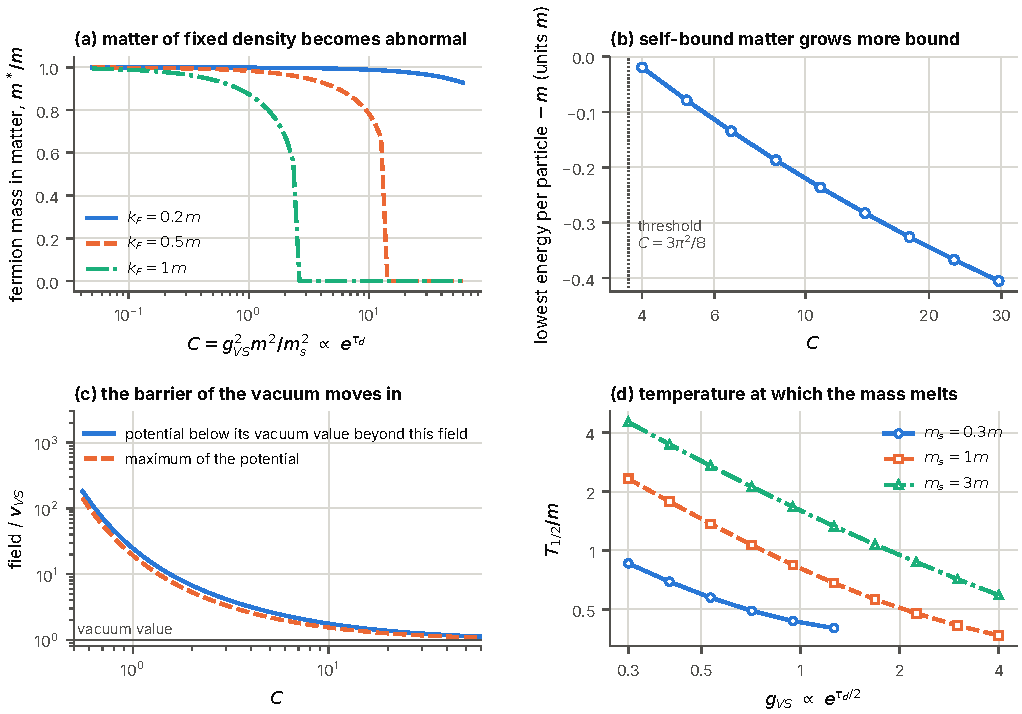
\includegraphics[width=0.92\textwidth]{fig_matter_history}
\caption{\label{fig:matter}Matter, vacuum and temperature along the clock. (a) The fermion mass in
matter of three fixed densities against $C\propto e^{\td}$: it drops to zero at the critical value.
(b) The lowest energy per particle of self-bound matter, minus $m$. (c) The field at which the
one-loop potential of the vacuum has its maximum, and the field beyond which it lies below the vacuum
value, in units of the vacuum value. (d) The temperature at which the fermions have lost half of
their mass, against the coupling, for three ratios $m_s/m$.}
\end{figure*}

\section{Order parameter, hidden symmetry and vortices}
\label{sec:order}

\subsection{Frame components and coordinate components}

The order parameter of the superfluid is the expectation value $\Delta^{a}$ of the vector pair
operator (\ref{eq:pairs}) along the extra axis $a\in\{0,5,6,7\}$: four complex numbers. On the
deflating spacetime the index $a$ is a \emph{frame} index: $\Delta^{a}$ is the component along the
unit vector $e_a$. The coordinate components along the deflating coordinates are
$\Delta_t=b_t(x4)\,\Delta^{t}$, and they shrink with the scale factors when the frame components are
constant. All statements below are about frame components.

The energy of the paired state depends on the order parameter through the $8\times8$ gap matrix
$\MM$ on the internal states of a pair. The identity of the earlier paper,
\begin{equation}
\tfrac18\,\mathrm{Tr}\big[(\MM\MM^\dagger)^{2}\big]
=2\Big(\sum_a|\Delta^{a}|^{2}\Big)^{2}-\Big|\sum_{a,b}\eta_{ab}\,\Delta^{a}\Delta^{b}\Big|^{2},
\label{eq:quartic}
\end{equation}
holds on the deflating spacetime with the frame metric $\eta_{ab}$ of the four axes, to
$2\times10^{-14}$. In coordinate components the same expression contains the metric $g_{tt}$ of the
moment.

\subsection{The ground state: no direction is preferred}

\begin{table}
\caption{\label{tab:states}The potential $V$ of the paired state for six states of the order
parameter, in units of $N(0)\Delta_F^{2}$, where $\Delta_F$ is the gap of a unitary state. Each
state is taken at the magnitude of the order parameter at which its potential is stationary.
$d_-^{2}$ and $d_+^{2}$: the squares of the two fourfold gaps of the state, in units of
$\Delta_F^{2}$. Flat and positive: the numbers of eigenvalues of the matrix of second derivatives of
the potential that vanish and that are positive.}
\begin{ruledtabular}
\begin{tabular}{p{0.37\columnwidth}ccccc}
state & $d_-^{2}$ & $d_+^{2}$ & $V$ & flat & positive \\
\hline
pair along the frame axis of $x0$ (hidden-axis singlet) & 1.000 & 1.000 & $-2.0000$ & 4 & 4 \\
pair along the frame axis of $x5$ & 1.000 & 1.000 & $-2.0000$ & 4 & 4 \\
pair along the frame axis of $x7$ & 1.000 & 1.000 & $-2.0000$ & 4 & 4 \\
unitary, rotated between $x0$ and $x5$ & 1.000 & 1.000 & $-2.0000$ & 4 & 4 \\
unitary, general direction and phase & 1.000 & 1.000 & $-2.0000$ & 4 & 4 \\
half-paired: $\eta_{ab}\Delta^a\Delta^b=0$ & 0.000 & 1.000 & $-1.0000$ & --- & --- \\
\end{tabular}
\end{ruledtabular}
\end{table}

Table~\ref{tab:states} gives the potential of the paired state for six states of the order
parameter. Every \emph{unitary} state, in which $\Delta^{a}$ is a real unit vector times a phase, has
all eight gaps equal and the lowest potential, whichever direction the vector has. It has four flat
directions, the Goldstone modes (one phase and three rotations of the direction), and four
directions of positive curvature. The \emph{half-paired} states, in which four of the eight gaps
vanish, have half the condensation energy.

One might have expected the deflation to select the direction of the order parameter: the hidden
axis $x0$, which does not deflate, against the three axes that do. \emph{In the sector of fields
that do not depend on the extra coordinates it does not.} The reason is the central observation of
Sec.~\ref{sec:dirac}: in this sector the weighted field obeys the flat equations, and their internal
symmetry rotates the four frame axes into one another. The symmetry of the manifold of ground states
is larger than the symmetry of the spacetime.

\subsection{The internal symmetry of the sector, and the symmetries of the spacetime}
\label{sec:hidden}

For fields that depend on $x1,x2,x3,x4$ only, the equation of the weighted field contains five
matrices: $\alpha^{1},\alpha^{2},\alpha^{3}$,
$\beta$ and $i\beta\chi$, the last through the coupling of the phase mode. The matrices that commute
with all five generate the \emph{internal symmetry} of the sector. The program computes it again for
the deflating spacetime, item by item, and finds it unchanged:
\begin{itemize}
\item the algebra is $su(2)_A\oplus su(2)_B\oplus u(1)_F\oplus u(1)_E$, of dimension 8;
\item the eight internal states of a fermion form the two doublets $(2,1)+(1,2)$;
\item the four vector pair operators (\ref{eq:pairs}) form the $(2,2)$, with fermion number 2, and
their one invariant quadratic form is the frame metric of the four axes, with the signs
$(+,+,+,+)$ up to an overall sign;
\item a condensate along one axis breaks $SO(4)=[SU(2)_A\times SU(2)_B]/Z_2$ to $SO(3)$.
\end{itemize}
Here $U(1)_E$ is a second phase symmetry of the sector, with a generator $P$ that has the square one
and distinguishes the doublets of $SU(2)_A$ from those of $SU(2)_B$.

Six of the generators are the products $\gamma^{A}\gamma^{B}$ of the six pairs taken from the four
axes $x0,x5,x6,x7$.
On the flat $7{+}1$ spacetime they are the rotations of the four extra space-like coordinates, and the
internal symmetry $SO(4)$ is a symmetry of the spacetime. On the deflating spacetime this is no
longer so (Fig.~\ref{fig:isometries}). Of the six, the spacetime keeps
\begin{itemize}
\item none, if the three rates differ;
\item one, the rotation of the two coordinates with the same rate, if two rates are equal;
\item three, the rotations of $x5,x6,x7$ among themselves, if the three rates are equal.
\end{itemize}
The three rotations that mix the hidden axis $x0$ with a deflating coordinate are never symmetries
of the deflating spacetime: $x0$ keeps its size and the other three shrink. The generators that are
lost as symmetries of the spacetime remain exact symmetries of the sector. They are \emph{hidden
symmetries}: symmetries of the equations of a sector that are not transformations of the spacetime.
The companion paper shows that on the $4{+}4$ spacetime this was the situation from the start
\cite{CompanionDefl1644,Flat1644}.

\subsection{Vortices and their zero modes}
\label{sec:vortex}

Because the vacuum value of the Vorton-Scalar breaks the phase symmetry $\UVS$, the field has
line-like defects \cite{NielsenOlesen1973}: along a straight line, say the $x3$ axis, its magnitude
vanishes, and around the line its phase winds by $2\pi$ times an integer. For unit winding,
$\PhiVS$ is $\vVS/\sqrt2$ times a profile that rises from 0 on the line to 1 at a distance of the
order of $1/m_s$, times $e^{i\theta_{12}}$ with the angle $\theta_{12}$ around the line in the plane
of $x1$ and $x2$.

\emph{Energy per unit length.} It is proportional to the square of the four-dimensional vacuum
value and so falls as $e^{-\td}$: in the four-dimensional description vortex lines become lighter as
the deflation proceeds, while their core, of the radius $1/m_s$, keeps its size.

\emph{Fermions on the line.} On the line the fermion mass vanishes, and fermions can be trapped
there \cite{JackiwRossi1981}. In the field of the vortex the Hamiltonian of a fermion is
\begin{equation}
\sum_{j=1}^{3}\alpha^{j}p_j+m\,(\text{profile})\,\beta\,\big(\cos\theta_{12}+i\chi\,\sin\theta_{12}\big),
\end{equation}
with the momenta $p_j$ along $x1,x2,x3$. A state of zero energy at zero momentum along the line is a
constant spinor $w_z$ times a function that decays away from the line. Inserting this form, the
Hamiltonian annihilates the state for every angle if and only if
\begin{equation}
\big(i\alpha^{1}+\beta\big)\,w_z=0,\qquad\big(i\alpha^{2}+i\beta\chi\big)\,w_z=0 .
\label{eq:zeromode}
\end{equation}
The five matrices $\alpha^{1},\alpha^{2},\alpha^{3},\beta,i\beta\chi$ are Hermitian, have the square
one and anticommute with one another. The two conditions state that $w_z$ is an eigenvector, with the
eigenvalue $-1$, of the two commuting matrices $i\beta\alpha^{1}$ and $\alpha^{2}\beta\chi$, and each
joint eigenspace of these two matrices has the dimension $16/4=4$. \emph{A vortex line of unit
winding carries four zero modes of the sixteen-component field.}

For a momentum $p_3$ along the line the energy is the eigenvalue of $\alpha^{3}p_3$. On the four
zero modes $\alpha^{3}$ equals the matrix
\begin{equation}
P_c=i\,\alpha^{1}\alpha^{2}\alpha^{3}\chi,
\end{equation}
the product of the five matrices, which commutes with each of them, is Hermitian and traceless and
has the square one; it is, up to its sign, the generator $P$ of $U(1)_E$. Its trace on the four zero
modes vanishes. \emph{Two zero modes move along the line in one direction at the speed of light and
two in the other}, and the direction of motion is tied to the charge under $U(1)_E$. For winding $-1$
the two directions are exchanged.

Equations (\ref{eq:zeromode}) contain only the matrices of the frame and the fermion mass, neither of
which changes. The four zero modes therefore exist at every moment of the deflation. The count also
holds on flat spacetime, where it corrects the earlier paper \cite{Flat1671}: that
paper quoted the count for a four-component field, one zero mode for each unit of winding, whereas
the sixteen components are equivalent to four such fields.

Massless fermions that run along a vortex line carry a current \cite{Witten1985}; a closed loop of
the line can be held open by that current, and such loops are the \emph{vortons} of the literature
on cosmic strings \cite{DavisShellard1989}. Because the energy per length of the line falls as
$e^{-\td}$ while the fermions on it stay massless, the balance between the tension of a loop and the
current on it shifts in favor of the current as the deflation proceeds. This paper establishes the
ingredients of that statement; it does not compute the equilibrium radius of a loop.

\section{Cosmology}
\label{sec:cosmo}

Hypothesis H3 says that the superfluid explains the dark matter, or the Hubble tension, or both. The
earlier paper examined it with the extra coordinates static. It found that the dark radiation of the
model does not relieve the Hubble tension and that a superfluid of the fermions cannot be the dark
matter of galaxies, although heavy bound pairs could be cold dark matter of an ordinary kind
\cite{Flat1671}. This section examines what changes when $x5,x6,x7$ deflate.
The deflation enters cosmology in several ways, and each requires an assumption beyond the
hypothesis of deflation. The assumptions are stated first and are kept apart throughout, so that the
reader can see which conclusion rests on which.

\subsection{Assumptions, and the equation of the expansion}

\emph{A1: ordinary space expands.} The coordinates $x1,x2,x3$ carry the scale factor
$a_{\mathrm{sp}}(x4)$ of standard cosmology, with the Hubble rate $H=d\ln a_{\mathrm{sp}}/dx4$; the
hidden coordinate $x0$ is static; $x5,x6,x7$ deflate at constant rates. The metric of
Sec.~\ref{sec:geometry} is the case $a_{\mathrm{sp}}=1$.

\emph{A2: gravity is the Einstein theory in eight dimensions}, with a constant $G_8$. The constant
of gravitation that an observer in ordinary space measures is then $G_8$ divided by the proper volume
of the extra coordinates,
\begin{equation}
\GN(x4)\ \propto\ \frac{1}{\Vd}\ \propto\ e^{\gsum\,x4},\qquad\frac{1}{\GN}\frac{d\GN}{dx4}=\gsum .
\label{eq:GN}
\end{equation}
Newton's constant \emph{grows} as the extra volume shrinks: gravity was weaker in the past. That a
changing volume of extra dimensions makes the constants of four dimensions change, and that
nucleosynthesis bounds the change, was pointed out long ago \cite{KolbPerryWalker1986}; for a review
of varying constants see Ref.~\cite{Uzan2011}. By Sec.~\ref{sec:egb}, A2 is an assumption that the
deflating spacetime itself puts in doubt: without matter the metric solves the equations of
Einstein-Gauss-Bonnet gravity, not Einstein's.

For a diagonal metric whose seven directions other than the time have the rates $H,H,H$ (ordinary
space), $0$ (the coordinate $x0$) and $-\gff,-\gss,-\gvv$, the component of Einstein's equations
along the time is the sum of the products of all pairs of rates, set equal to $8\pi G_8$ times the
energy density in eight dimensions. Dividing the density by the extra volume turns $G_8$ into $\GN$:
\begin{equation}
3H^{2}-3\,\gsum\,H+\gprod=8\pi\,\GN(x4)\,\rho,
\label{eq:friedmann}
\end{equation}
with the density $\rho$ of radiation, matter and the cosmological term in ordinary space. For the
unperturbed universe Eq.~(\ref{eq:friedmann}) is the only one of Einstein's equations that is
needed. The others determine the stresses of the unknown source that keeps the three rates constant;
they enter when ordinary space is perturbed (Sec.~\ref{sec:pert}).

The calculations take three equal rates, so that $\gprod=\gsum^{2}/3$, and the densities of the
standard model of cosmology \cite{Planck2018VI} as the earlier paper used them: baryons
$\omega_b=0.02237$, cold dark matter $\omega_c=0.1200$, and $H_0=67.36~\kmsMpc$ without deflation.
The cosmological term is chosen so that Eq.~(\ref{eq:friedmann}) holds today. Without deflation the
program reproduces the two numbers of the earlier calculation on which this section rests: the angle
$\theta_*$ under which the sound horizon at last scattering is seen, $100\,\theta_*=1.03965$, and
that sound horizon, $r_s=144.449$~Mpc.

\subsection{The Hubble constant inferred from the sound horizon}

The microwave background fixes the angle $\theta_*$ to high precision. A model that changes the history of the expansion must keep that angle,
and the Hubble constant that it then requires is the \emph{inferred} Hubble constant. The tension is
that the standard model infers $67.4~\kmsMpc$ \cite{Planck2018VI} while the local distance network
measures $73.50\pm0.81$ \cite{H0DN2026}. Table~\ref{tab:hubble} gives the inferred value on the
deflating spacetime under A1 and A2, at fixed $\theta_*$ and fixed densities of baryons and dark
matter. The redshift $z_*$ of last scattering and the mass fraction $\YHe$ of helium, which the sound
horizon needs, are computed on the deflating background (Sec.~\ref{sec:spectra}).

\begin{table*}
\caption{\label{tab:hubble}The Hubble constant inferred from the angular scale of the sound horizon
if Newton's constant grows with the deflation (assumptions A1 and A2). $\GN$ ratio: Newton's constant
in the early universe divided by its value today, $e^{-\gsum\,t_0}$ with the age $t_0$ of the model.
$z_*$: redshift of last scattering; $\YHe$: mass fraction of helium. Last column: the Hubble constant
that results if $z_*$ and $\YHe$ are held at their values without deflation.
The rows at $\gsum/H_0=0.00324$ and $0.0644$ are the bounds of lunar laser ranging and of
nucleosynthesis (Table~\ref{tab:bounds}).}
\begin{ruledtabular}
\begin{tabular}{cccccccccc}
$\gsum/H_0$ & $\gsum$ (per year) & $H_0$ ($\kmsMpc$) & change & $\GN$ ratio & $z_*$ & $\YHe$ & $r_s$ (Mpc) & $t_0$ (Gyr) & $H_0$, $z_*$ and $\YHe$ held \\
\hline
0 & 0 & 67.36 & 0.00 & 1.0000 & 1089.92 & 0.2454 & 144.45 & 13.81 & 67.36 \\
0.00100 & $6.89\times10^{-14}$ & 67.29 & $-0.07$ & 0.9990 & 1089.90 & 0.2453 & 144.52 & 13.82 & 67.30 \\
0.00300 & $2.07\times10^{-13}$ & 67.16 & $-0.20$ & 0.9971 & 1089.86 & 0.2452 & 144.66 & 13.84 & 67.18 \\
0.00324 & $2.23\times10^{-13}$ & 67.15 & $-0.21$ & 0.9969 & 1089.86 & 0.2451 & 144.68 & 13.84 & 67.16 \\
0.0100 & $6.89\times10^{-13}$ & 66.70 & $-0.66$ & 0.9905 & 1089.73 & 0.2446 & 145.16 & 13.90 & 66.74 \\
0.0300 & $2.07\times10^{-12}$ & 65.36 & $-2.00$ & 0.9714 & 1089.37 & 0.2430 & 146.61 & 14.06 & 65.48 \\
0.0644 & $4.43\times10^{-12}$ & 62.98 & $-4.38$ & 0.9383 & 1088.72 & 0.2401 & 149.23 & 14.37 & 63.23 \\
0.100 & $6.89\times10^{-12}$ & 60.37 & $-6.99$ & 0.9037 & 1088.04 & 0.2370 & 152.13 & 14.70 & 60.77 \\
0.300 & $2.07\times10^{-11}$ & 41.94 & $-25.42$ & 0.6995 & 1083.78 & 0.2168 & 173.35 & 17.29 & 43.41 \\
\end{tabular}
\end{ruledtabular}
\end{table*}

\emph{The inferred Hubble constant falls}, with the slope $d\ln H_0/d(\gsum/H_0)=-0.969$ at small
rates. The reason is this. By Eq.~(\ref{eq:GN}) gravity was weaker in the early universe; the
universe expanded more slowly at a given density; sound had more time to travel, and the sound
horizon is larger. To keep the angle, the distance to last scattering must be larger, which requires
a smaller Hubble constant. The deflation moves the inferred value \emph{away} from the local
measurement [Fig.~\ref{fig:hubble}(a)]. Weaker gravity also delays last scattering and lowers the
helium fraction, because the universe expanded more slowly during recombination and during
nucleosynthesis as well; both enlarge the sound horizon further. If $z_*$ and $\YHe$ are held at
their values without deflation, the slope is $-0.911$: that simpler calculation underestimates the
fall by six per cent of itself. An independent calculation of recombination confirms both numbers
(Appendix~\ref{app:checks}). The term $\gprod$ of Eq.~(\ref{eq:friedmann}) plays no part
in this: it is of the second order in the rate, and it acts as a constant, which the cosmological
term that is adjusted to today's expansion absorbs almost exactly.

\begin{figure*}
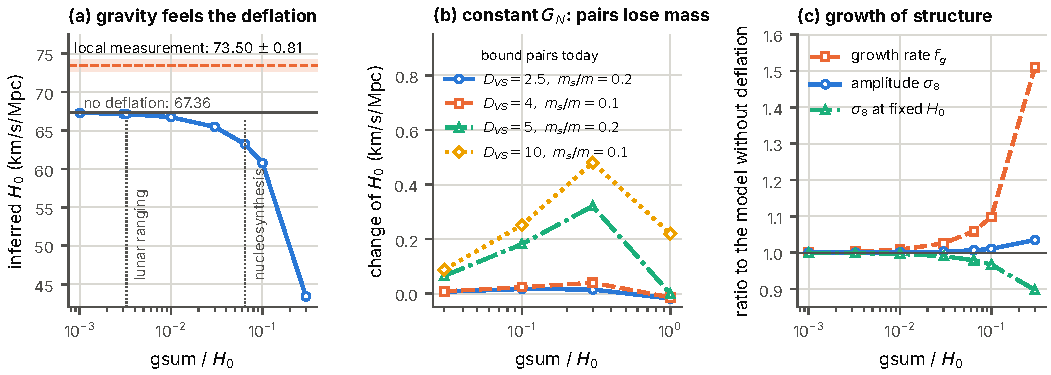
\includegraphics[width=\textwidth]{fig_hubble}
\caption{\label{fig:hubble}The Hubble constant and the growth of structure on a deflating spacetime.
(a) The Hubble constant inferred from the angular scale of the sound horizon against the rate of
deflation, if gravity feels the deflation (A1, A2): with recombination computed on the deflating
background, and with last scattering and the helium fraction held fixed; the bounds of
Table~\ref{tab:bounds} and the local measurement are marked. (b) The change of the inferred Hubble
constant if Newton's constant is held fixed and bound pairs lose rest mass. (c) Amplitude and rate of
the growth of structure relative to the model without deflation, at a fixed angle of the sound
horizon, for the two closures of Sec.~\ref{sec:pert}.}
\end{figure*}

\subsection{How fast can the coordinates deflate today?}

\begin{table*}
\caption{\label{tab:bounds}Upper bounds on the present total rate of deflation, each under the
assumption named. Uncertainties of the measured values are at 68 per cent unless stated; the bounds
are at two standard deviations. The bound in units of $H_0$ uses $H_0=67.36~\kmsMpc$. A2: gravity is
the Einstein theory in eight dimensions. HV: the vacuum value of the Vorton-Scalar sets the
electroweak scale. H2: the superfluid state is the Higgs field; the bound is given for $\nEW=1$ and
scales as $1/\nEW$ (Sec.~\ref{sec:higgs}).}
\begin{ruledtabular}
\begin{tabular}{p{0.17\textwidth}p{0.27\textwidth}p{0.15\textwidth}cc}
observation & measured & assumption & bound on $\gsum$ (per year) & in units of $H_0$ \\
\hline
lunar laser ranging \cite{HofmannMueller2018} & $(d\GN/dt)/\GN=(7.1\pm7.6)\times10^{-14}$ per year & A2 & $2.230\times10^{-13}$ & $3.237\times10^{-3}$ \\
nucleosynthesis, Newton's constant \cite{Alvey2020} & $\GN$ then, divided by $\GN$ today: $0.99^{+0.06}_{-0.05}$ (two standard deviations) & A2; constant rate & $4.434\times10^{-12}$ & 0.0644 \\
nucleosynthesis, Fermi constant \cite{ScherrerSpergel1993} & $G_{\mathrm{Fermi}}$ at $t=1$~s within 20 (10) per cent of today's value, at fixed fermion masses & HV; constant rate & $1.615\times10^{-11}$ ($7.627\times10^{-12}$) & 0.234 (0.111) \\
atomic clocks, mass ratio \cite{Lange2021} & $(d/dt)\ln(m_p/m_e)=(-8\pm36)\times10^{-18}$ per year & H2, $\nEW=1$ & $8.000\times10^{-17}$ & $1.161\times10^{-6}$ \\
atomic clocks, fine-structure constant \cite{Lange2021} & $(d\alpha_{\mathrm{em}}/dt)/\alpha_{\mathrm{em}}=(1.0\pm1.1)\times10^{-18}$ per year & an electromagnetic field along $x5,x6,x7$ (not part of the model) & $3.200\times10^{-18}$ & $4.645\times10^{-8}$ \\
\end{tabular}
\end{ruledtabular}
\end{table*}

Table~\ref{tab:bounds} and Fig.~\ref{fig:bounds} collect the bounds.

\emph{Under A2, lunar laser ranging} measures $(d\GN/dt)/\GN$ directly, and Eq.~(\ref{eq:GN}) turns
its limit into $\gsum<2.23\times10^{-13}$ per year, that is, $3.24\times10^{-3}\,H_0$. At this rate
the deflation clock has advanced by $\gsum\,t_0=3.1\times10^{-3}$ over the age $t_0$ of the universe,
and the inferred Hubble constant is lower by $0.21~\kmsMpc$.

\emph{Under A2, nucleosynthesis} bounds the ratio of Newton's constant then to its value today; for
a rate that was constant since, $\gsum<0.064\,H_0$. This is weaker than the first bound but does not
assume that the rate today equals the rate in the past.

\emph{Under HV, nucleosynthesis} bounds the change of the Fermi constant at fixed fermion masses to
10 to 20 per cent, which gives $\gsum<0.111$ to $0.234\,H_0$. HV is the assumption that the
Vorton-Scalar itself plays the role of the Higgs field, so that
$G_{\mathrm{Fermi}}=1/(\sqrt2\,\vVS^{2})$ grows as $e^{\td}$ while every mass stays constant. It is
\emph{not} the hypothesis H2, and the earlier paper already noted that the Vorton-Scalar, a singlet
of all non-Abelian symmetries, cannot be the Higgs field of the Standard Model; the bound is given
only to show what the assumption would imply.

\emph{Under the hypothesis H2, atomic clocks} give by far the strongest bound, and one that needs no
assumption about gravity. Section~\ref{sec:higgs} derives it: $\gsum<1.16\times10^{-6}\,H_0/\nEW$
with an exponent $\nEW$ of order one or larger.

\emph{The fine-structure constant} is bounded by the same clocks to parts in $10^{18}$ per year.
This would bound the rate, to $4.6\times10^{-8}\,H_0$, only if an electromagnetic field propagated
along the deflating coordinates. The model contains no electromagnetic field; the row shows how
strongly such an extension would be constrained.

\emph{Under A2, the microwave background} would bound the rate as well. Section~\ref{sec:forecast}
finds, as a forecast for mock data of the quality of the Planck satellite and not as a measurement,
$\gsum<0.0385\,H_0$; Fig.~\ref{fig:bounds} includes it for comparison.

\emph{In the model as it stands}, without H2, HV or an electromagnetic extension and without A2, no
mass and no coupling of ordinary matter depends on the deflation, and none of these observations
bounds the rate.

The consequence for the histories of Secs.~\ref{sec:gap} to \ref{sec:cjt} is severe. Under A2 the
clock has advanced by at most 0.0031 during the whole of cosmic history, if the rate was constant;
under H2 by at most $1.1\times10^{-6}/\nEW$. A history in which pairs become bound, matter loses its
fermion mass or the gap grows by orders of magnitude within the age of the universe requires that
gravity does not feel the deflation, that the superfluid is not the Higgs field, or that the rate
was much larger in the past than it is today.

\begin{figure*}
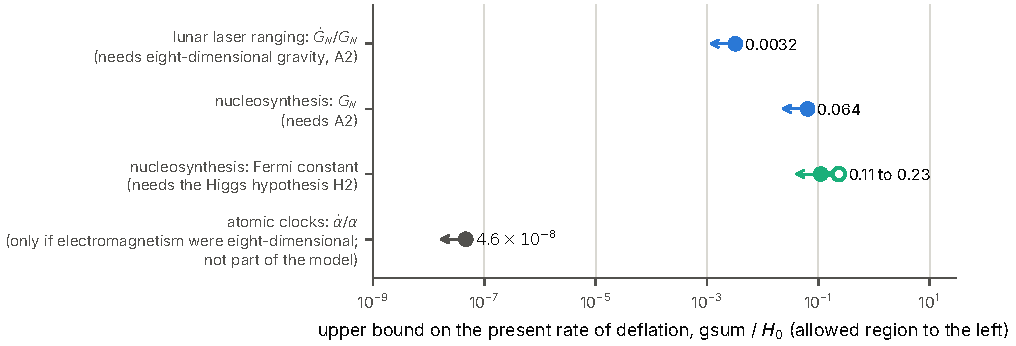
\includegraphics[width=0.8\textwidth]{fig_bounds}
\caption{\label{fig:bounds}Upper bounds on the present total rate of deflation in units of the
Hubble constant, each under the assumption of Table~\ref{tab:bounds}. The allowed region is to the
left of each bound. The row ``microwave background'' is not a measurement but the forecast of
Sec.~\ref{sec:forecast} for mock data (open symbol: Planck-like; filled symbol: with a deep
survey).}
\end{figure*}

\subsection{Bound pairs lose rest mass}

If the dark matter consists of bound pairs of the fermions, its particles have the rest mass $2m$
minus the binding energy. The binding energy grows with the coupling, so that the pairs become
lighter as the deflation proceeds, and the density of dark matter falls slightly faster than the
inverse volume. A dark matter that was heavier in the past raises the inferred Hubble constant. The
program computes the effect for four examples with $\aVS$ between 0.4 and 1 today, where the binding
energy is at most 8.2 per cent of the rest mass [Fig.~\ref{fig:hubble}(b)]. If gravity feels the
deflation, the inferred Hubble constant changes by between $-4.11$ and $-0.19~\kmsMpc$ at the rates
that nucleosynthesis and lunar laser ranging allow: the weaker gravity of the past outweighs the
loss of mass. (These examples hold $z_*$ and $\YHe$ fixed, which by Table~\ref{tab:hubble}
underestimates a fall by about six per cent of itself.) If Newton's constant is held fixed and the deflation acts on the dark sector alone,
rates between 0.03 and $1\,H_0$ raise the inferred Hubble constant by at most $+0.48~\kmsMpc$, for a
loss of up to 7.7 per cent of the rest mass. This is the only effect of the deflation found here
that raises the inferred Hubble constant, and in these examples it supplies less than a tenth of the
$6.1~\kmsMpc$ that separate the model from the local measurement.

\subsection{Perturbations of ordinary space: what must be assumed}
\label{sec:pert}

The quantities of the preceding subsections belong to the unperturbed universe. The growth of
structure and the spectra of the microwave background are built from small perturbations of
ordinary space, and the equations of the perturbations contain more of Einstein's equations than
Eq.~(\ref{eq:friedmann}). They therefore contain what the hypothesis of deflation leaves open.

\emph{The agent.} Something must keep the three rates constant while ordinary space expands and
matter dilutes. We call it the agent and assume nothing about its nature. Assumption A2 says that it
has no energy density: otherwise its density would stand on the right of Eq.~(\ref{eq:friedmann}).
It cannot be without stresses. The components of Einstein's equations along ordinary space, together
with the conservation of matter in ordinary space and Eq.~(\ref{eq:GN}), require the agent to have,
in ordinary space, the pressure
\begin{equation}
\begin{aligned}
8\pi\GN\,p_{\mathrm{agent}}={}&-\frac{\gsum}{H}\frac{dH}{dx4}-2\,\gsum\,H\\
&+2\,\gprod-\frac{\gsum\,\gprod}{3H}.
\end{aligned}
\label{eq:pagent}
\end{equation}
In an era of matter this is $-\gsum\,H/2$ to the first order in the rates. The agent is a medium
without energy density and with a tension, of the relative size $\gsum/H$. When ordinary space is
perturbed, such a medium will in general be perturbed too.

\emph{A3: the perturbations.} We assume (i) that in a universe with small inhomogeneities the scale
factors $b_t$ of the deflating coordinates remain the prescribed functions of the time, the time
being the proper time of observers who move with the cold matter, and that $x0$ remains static; and
(ii) that the agent has no energy density in the perturbed universe either. Part (i) is the plainest
reading of the hypothesis of deflation in a universe that is not exactly homogeneous; part (ii) is
A2 taken to first order. Both are assumptions.

\emph{The equations.} We use the conformal time $\tcf$ of ordinary space, defined by
$d\tcf=dx4/a_{\mathrm{sp}}$, write a prime for the derivative with respect to it, and write
$\Hcf=a_{\mathrm{sp}}'/a_{\mathrm{sp}}=a_{\mathrm{sp}}H$ for the conformal Hubble rate. A scalar
perturbation of ordinary space with the comoving wavenumber $k$ is described, in the synchronous
gauge, by two functions $\hsy(\tcf)$ and $\etasy(\tcf)$ of the perturbed metric; they are the $h$
and $\eta$ of Ref.~\cite{MaBertschinger1995}, written here with an index because $h$ and $\eta$ have
other meanings in this paper. The combination
$\alsy=(\hsy'+6\,\etasy')/2k^{2}$ occurs repeatedly. Matter and radiation enter through four sums
over the species, each multiplied by $8\pi\GN(x4)\,a_{\mathrm{sp}}^{2}$ with the Newton's constant of
the moment: $\cD$, the perturbation of the energy density; $\cT$, the divergence of the momentum
density; $\cP$, the perturbation of the pressure; and $\cA$, the anisotropic stress. With the scale
factors of the extra coordinates unperturbed, the Einstein tensor of the eight-dimensional metric
gives, to first order,
\begin{subequations}
\label{eq:pert}
\begin{align}
2k^{2}\etasy-\He\,\hsy'&=-\cD,\label{eq:E}\\
2k^{2}\etasy'&=\cT,\label{eq:M}\\
\hsy''+2\He\,\hsy'-2k^{2}\etasy&=-3\,\cP,\label{eq:T}\\
\alsy'+2\He\,\alsy-\etasy&=-\tfrac32\,\cA/k^{2},\label{eq:S}
\end{align}
\end{subequations}
with
\begin{equation}
\He=\Hcf-\tfrac12\,a_{\mathrm{sp}}\,\gsum .
\label{eq:He}
\end{equation}
They are the energy constraint, the momentum constraint, the trace of the space-space equations and
their traceless part, the equation of the shear. An independent program derives them by computer
algebra for arbitrary rates and for both signatures (Appendix~\ref{app:checks}). They are the four
equations of general relativity \cite{MaBertschinger1995} with two changes: Newton's constant is
that of the moment, and $\Hcf$ is replaced by $\He$ in three of them. The second change can be read
off Eq.~(\ref{eq:friedmann}). The time component of the Einstein tensor is the sum of the products
of all pairs of expansion rates. If the rate of one ordinary direction is perturbed, the
perturbation multiplies the sum of the rates of all \emph{other} directions, which is $2H$ in four
dimensions and $2H-\gsum$ here.

\emph{The four equations cannot all hold with matter alone.} In general relativity two of the four
equations (\ref{eq:pert}) imply the other two, because the energy and the momentum of matter are
conserved. Here they do not. Let Eq.~(\ref{eq:E}) hold, and define three \emph{gaps}, the amounts by
which the other three fail when only matter and radiation stand on their right-hand sides:
\begin{equation}
\begin{aligned}
\cYM&=2k^{2}\etasy'-\cT,\\
\cYT&=\hsy''+2\He\,\hsy'-2k^{2}\etasy+3\,\cP,\\
\cYS&=\alsy'+2\He\,\alsy-\etasy+\tfrac32\,\cA/k^{2}.
\end{aligned}
\label{eq:gaps}
\end{equation}
The conservation of the energy and of the momentum of matter in ordinary space gives two identities
between them,
\begin{align}
\cYM&=\He\,\cYT+\cZ,\label{eq:id1}\\
2k^{2}\,\cYS&=\cYT+\frac{3}{k^{2}}\big(\cYM'+2\He\,\cYM\big),\label{eq:id2}
\end{align}
with
\begin{equation}
\begin{aligned}
\cZ&=\hsy'\,\cB-\tfrac12\,a_{\mathrm{sp}}\,\gsum\,(\cD-3\,\cP),\\
\cB&=\He'-\He^{2}+\tfrac12(\cE+\cE_P).
\end{aligned}
\label{eq:Z}
\end{equation}
Here $\cE$ and $\cE_P$ are $8\pi\GN a_{\mathrm{sp}}^{2}$ times the density and the pressure of the
unperturbed universe. By Eq.~(\ref{eq:friedmann}) the quantity $\cB$ is proportional to $\gsum$; in
an era of matter it is $a_{\mathrm{sp}}\,\gsum\,\Hcf/4$. Without deflation $\cB$ and $\cZ$ vanish,
and Eqs.~(\ref{eq:id1}) and (\ref{eq:id2}) say that if one gap vanishes at all times, all three do:
that is general relativity. With deflation $\cZ\neq0$, and \emph{the three gaps cannot all vanish}.
This is not a defect of the calculation. It is the statement that the agent, which has a tension,
takes part in the perturbations: the gaps are, up to the factor $8\pi\GN a_{\mathrm{sp}}^{2}$, the
perturbations of its momentum density, of its pressure and of its anisotropic stress.

\emph{Closures.} The two identities relate three gaps; one more relation closes the system, and the
hypothesis offers no ground for a choice. Three natural choices set one gap to zero. In the closure
``Momentum'', $\cYM=0$: the agent carries no momentum density, and
Eqs.~(\ref{eq:E}) and (\ref{eq:M}) hold. In the closure ``Pressure'', $\cYT=0$: the agent carries no
perturbation of its pressure, Eqs.~(\ref{eq:E}) and (\ref{eq:T}) hold, and Eq.~(\ref{eq:M}) is
replaced by $2k^{2}\etasy'=\cT+\cZ$. In the closure ``Shear'', $\cYS=0$: the agent carries no
anisotropic stress, as a perfect fluid or a scalar field would not. Eliminating $\cYT$ from the two
identities then gives an equation of motion for the momentum density of the agent,
\begin{equation}
\cYM'=-\Big(\frac{k^{2}}{3\He}+2\He\Big)\cYM+\frac{k^{2}}{3\He}\,\cZ .
\label{eq:shearclosure}
\end{equation}
Far inside the horizon, $k\gg\Hcf$, the rate $k^{2}/3\He$ is enormous, and $\cYM$ relaxes at once to
$\cZ$, its value in the closure ``Pressure''. \emph{Inside the horizon the closure ``Shear'' is the
closure ``Pressure''}, with corrections of the relative order $(\Hcf/k)^{2}$. We compute with the
closures ``Momentum'' and ``Pressure'' and mark every result as depending on the closure or not.

All gaps are proportional to $a_{\mathrm{sp}}\,\gsum/\Hcf=\gsum/H$. At the largest rate that
nucleosynthesis allows this ratio is $2.7\times10^{-6}$ at recombination and $6.9\times10^{-2}$
today. The closure therefore cannot matter for anything that is decided at recombination, and it
must matter for the gravitational potentials and for the growth of structure of the recent universe.

\subsection{The growth of structure}

For pressureless matter with the density contrast $\delta_m$ and the density $\rho_m$ each closure
gives one equation. In the closure ``Pressure'', Eqs.~(\ref{eq:E}) and (\ref{eq:T}) give
\begin{equation}
\frac{d^{2}\delta_m}{dx4^{2}}+\Big(2H-\frac{\gsum}{2}\Big)\frac{d\delta_m}{dx4}=4\pi\,\GN(x4)\,\rho_m\,\delta_m :
\label{eq:growthP}
\end{equation}
gravity is that of the moment, and the Hubble friction is reduced by $\gsum/2$. In the closure
``Momentum'', the derivative of Eq.~(\ref{eq:E}) with Eq.~(\ref{eq:M}) gives, in conformal time,
\begin{equation}
\delta_m''+\frac{2\He'+\cE_m+\tfrac43\cE_r}{2\He}\,\delta_m'=\frac{\Hcf-a_{\mathrm{sp}}\,\gsum}{2\He}\,\cE_m\,\delta_m ,
\label{eq:growthM}
\end{equation}
where $\cE_m$ and $\cE_r$ are the parts of $\cE$ from matter and from radiation. Here the source is
reduced as well, by the factor $(H-\gsum)/(H-\gsum/2)$. (The term with $\cE_r$ is the momentum
density of radiation that streams freely: far inside the horizon its velocity divergence is
$-\hsy'/2$ \cite{MaBertschinger1995}.) Without deflation both equations reduce to the familiar
$d^{2}\delta_m/dx4^{2}+2H\,d\delta_m/dx4=4\pi\GN\rho_m\delta_m$. With deflation that familiar
equation, with $\GN(x4)$ inserted, is neither of the two. For matter alone and three equal rates the
growth rate $d\ln\delta_m/d\ln a_{\mathrm{sp}}$ is, to the first order in $\gsum/H$,
$1-\tfrac{9}{16}\,\gsum/H$ in the closure ``Pressure'' and $1-\tfrac{13}{16}\,\gsum/H$ in the closure
``Momentum''.

Two effects oppose each other [Fig.~\ref{fig:hubble}(c)]. At a \emph{fixed} Hubble constant, weaker
gravity in the past lowers the amplitude $\sigma_8$ of clustering today:
$d\ln\sigma_8/d(\gsum/H_0)=-0.443$ in the closure ``Momentum'' and $-0.207$ in the closure
``Pressure''. But the Hubble constant that keeps the angle of the sound horizon is lower, the
cosmological term takes over later, and matter clusters for longer. With that Hubble constant the net
change is $+0.003$ and $+0.239$ per unit of $\gsum/H_0$: $+0.001$ and $+0.077$ per cent at the bound
of lunar laser ranging, and $+0.01$ and $+1.60$ per cent at the bound of nucleosynthesis. The growth
rate today, $f_g=d\ln\delta_m/d\ln a_{\mathrm{sp}}$, rises in both closures, by the factors 1.0021
and 1.0035 at the first bound and 1.0463 and 1.0773 at the second. Common to both closures is that,
at a fixed angle, the amplitude does not fall and the growth rate rises. How large the changes are
depends on the closure: \emph{the growth of structure on the deflating spacetime is not predicted
until the perturbations of the agent are specified.}

\subsection{The spectra of the microwave background}
\label{sec:spectra}

\emph{The program.} The earlier paper computed the temperature and polarization spectra of the
microwave background and the power spectrum of matter with an Einstein-Boltzmann program of its own
\cite{Flat1671}. That program has Newton's constant built into its units. For the
deflating spacetime four of its parts were copied and changed in a short, listed set of places: the
expansion obeys Eq.~(\ref{eq:friedmann}); every source of the metric perturbations carries the
Newton's constant of the moment; the energy constraint is Eq.~(\ref{eq:E}); and the sources of the
temperature anisotropy contain the gap $\cYS$ of the closure. The equations of motion of photons,
neutrinos, baryons and dark matter are not changed: matter that is spread uniformly over the extra
coordinates moves in ordinary space as it does in four dimensions, and Thomson scattering and
recombination are atomic physics, which the model does not alter. The copies are written by a script
from the original files, so that they cannot differ from them in any place that is not listed, and
without deflation they reproduce the spectra of the earlier paper to the last binary digit.

\emph{Recombination and helium.} Recombination is computed on the expansion history of
Eq.~(\ref{eq:friedmann}), with the three-level atom and its standard corrections
\cite{SeagerSasselovScott1999}. The helium fraction responds as well. At nucleosynthesis Newton's
constant was smaller than today by the factor $\GN$ ratio of Table~\ref{tab:hubble}; a universe that
expands more slowly by that factor in $H^{2}$ is equivalent, for nucleosynthesis, to one with
$\tfrac{43}{7}(\GN\ \text{ratio}-1)$ additional neutrino species, a negative number, and the helium
fraction follows from the standard fit \cite{Planck2015XIII}. (In a model with extra radiation,
$\tfrac{43}{7}$ is replaced by $\tfrac{43}{7}+\Delta N$, where $\Delta N$ is the density of that
radiation during nucleosynthesis in units of one neutrino species.) At the largest rate that
nucleosynthesis allows, and without extra radiation, this is $-0.379$ species, and $\YHe$ falls
from 0.24540 to 0.24008.

\emph{Spectra at a fixed angle.} Table~\ref{tab:spectra} lists the model without deflation and
five models with three equal rates, each with the densities, the primordial amplitude and tilt and the optical depth of the standard
model and with the Hubble constant that keeps $100\,\theta_*=1.03965$. Keeping the angle keeps the
acoustic peaks in place: the first five move by at most 0.32 in the multipole $\ell$. What changes is
their height and the damping tail [Fig.~\ref{fig:spectra}], for the reasons that apply to any change
of the expansion rate at recombination: the ratio of the diffusion length to the sound horizon, the
width of the last-scattering surface and the decay of the potentials shortly after recombination all
change, and the lower helium fraction leaves more electrons per baryon.

\begin{table*}
\caption{\label{tab:spectra}Spectra of the microwave background on the deflating spacetime at a fixed
angle of the sound horizon (assumptions A1, A2, A3; three equal rates). $H_0$ in $\kmsMpc$.
$\GN(z_*)/\GN$: Newton's constant at last scattering divided by its value today. $\sigma_8$:
amplitude of clustering for the same primordial amplitude, in the closures ``Momentum'' (M) and
``Pressure'' (P). Largest change: of the temperature spectrum $D_\ell^{TT}$ for $30\le\ell\le2500$
relative to the model without deflation. Ideal measurement: the root of the sum over those
multipoles of the squared change divided by the variance $2/(2\ell+1)$ of one multipole, that is,
the number of standard deviations by which a measurement of the temperature on the whole sky without
noise would tell the model from no deflation if nothing else were unknown. $\Delta\chi^{2}$: against
Planck-like mock data with all other parameters fixed.}
\begin{ruledtabular}
\begin{tabular}{cccccccc}
$\gsum/H_0$ & $H_0$ & $\GN(z_*)/\GN$ & $\sigma_8$ (M) & $\sigma_8$ (P) & largest change & ideal measurement & $\Delta\chi^{2}$ \\
\hline
0 & 67.360 & 1.0000 & 0.8228 & 0.8228 & 0 & 0.0 & 0.00 \\
0.00324 & 67.149 & 0.9969 & 0.8219 & 0.8225 & $2.7\times10^{-3}$ & 3.1 & 1.12 \\
0.0100 & 66.704 & 0.9905 & 0.8200 & 0.8219 & $8.3\times10^{-3}$ & 9.7 & 10.79 \\
0.0300 & 65.365 & 0.9714 & 0.8142 & 0.8201 & 0.025 & 29.5 & 98.85 \\
0.0644 & 62.976 & 0.9383 & 0.8032 & 0.8160 & 0.056 & 64.8 & 468.30 \\
0.100 & 60.368 & 0.9037 & 0.7903 & 0.8104 & 0.090 & 103.5 & 1166.70 \\
\end{tabular}
\end{ruledtabular}
\end{table*}

At the rate that lunar laser ranging allows, the temperature spectrum differs from that of the
model without deflation by at most $2.7\times10^{-3}$ of itself, 0.134 of the cosmic variance of a
single multipole, and $\Delta\chi^{2}=1.12$ against Planck-like mock data
(Sec.~\ref{sec:forecast}) before any parameter is refitted. Such data cannot tell this rate from no
deflation. At the rate that nucleosynthesis allows, Newton's constant at last scattering was 0.9383
of today's, the spectrum changes by up to 5.6 per cent, and $\Delta\chi^{2}=468$: the microwave
background is then a stronger test than nucleosynthesis.

\begin{figure*}
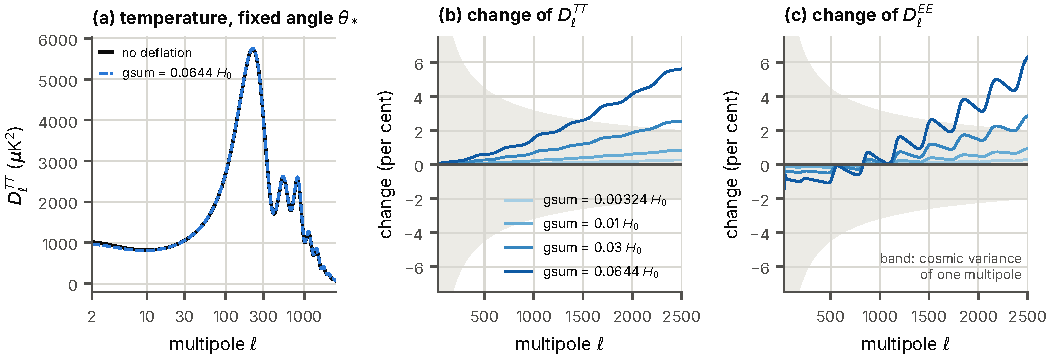
\includegraphics[width=\textwidth]{fig_spectra}
\caption{\label{fig:spectra}The spectra of the microwave background at a fixed angle of the sound
horizon. (a) The temperature spectrum without deflation and at the largest rate that nucleosynthesis
allows. (b), (c) The change of the temperature and polarization spectra relative to the model
without deflation for four rates (darker: faster); the band is the cosmic variance of a single
multipole. Closure ``Momentum''; at these multipoles the closure ``Pressure'' gives the same
curves.}
\end{figure*}

\emph{The closure.} For $30\le\ell\le2500$ the spectra of the two closures differ by a thousandth of
the effect of the deflation itself ($1.4\times10^{-3}$ and $1.2\times10^{-3}$ of it at the two
bounds), and $\Delta\chi^{2}$ is the same to five digits [Fig.~\ref{fig:closure}(a)]. \emph{The
spectra at these multipoles follow from A1, A2 and A3, whatever the closure.} For
$\ell<30$, where the potentials of the recent universe act through the late integrated Sachs-Wolfe
effect, the closures differ by more than the effect of the deflation in either of them, by a factor
2.1. The largest angular scales are not predicted; their cosmic variance is large, and at the rate
of nucleosynthesis the closures differ by at most a third of it. The amplitude of matter is 0.9762
of its value without deflation in the closure ``Momentum'' and 0.9918 in the closure ``Pressure'' at
the rate of nucleosynthesis, and 0.99892 and 0.99969 at the rate of lunar laser ranging.

Figure~\ref{fig:closure}(b) shows what the agent must supply. In units of $a_{\mathrm{sp}}\,\gsum/\Hcf$
times the terms of each equation, the closure ``Momentum'' lacks 0.54 to 0.98 in Eq.~(\ref{eq:T}) and
0.31 to 0.49 in Eq.~(\ref{eq:S}) after recombination; the closure ``Pressure'' lacks 0.62 to 0.94 in
Eq.~(\ref{eq:M}), and in Eq.~(\ref{eq:S}) an amount that falls as $(\Hcf/k)^{2}$ inside the horizon,
as Eq.~(\ref{eq:shearclosure}) requires. The two identities (\ref{eq:id1}) and (\ref{eq:id2}) hold
along the numerical solutions to $8.6\times10^{-4}$, the accuracy of the numerical derivative with
which they are tested. The complete calculation, with photons, neutrinos and baryons, reproduces the
growth of Eqs.~(\ref{eq:growthP}) and (\ref{eq:growthM}) to $1.3\times10^{-4}$
[Fig.~\ref{fig:closure}(c)]; with the equation of the other closure it would disagree by a quarter
of $\gsum/H_0$.

\begin{figure*}
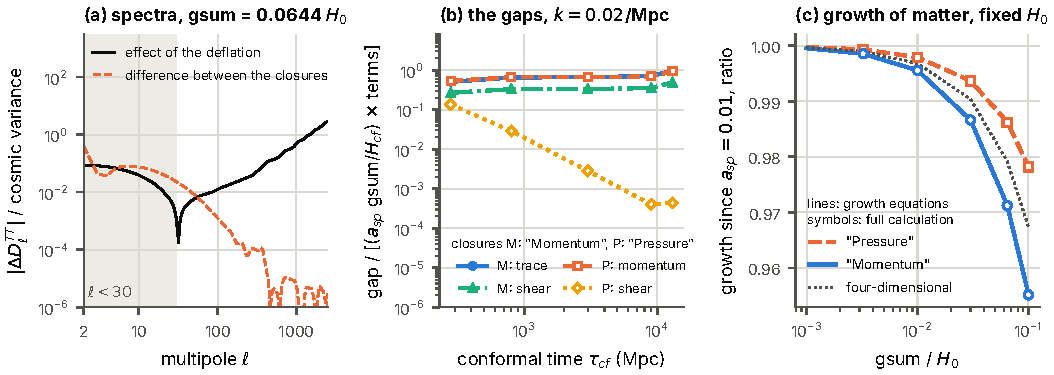
\includegraphics[width=\textwidth]{fig_closure}
\caption{\label{fig:closure}The closure of the perturbation equations, at the largest rate that
nucleosynthesis allows. (a) The difference between the temperature spectra of the closures
``Momentum'' and ``Pressure'', and the effect of the deflation itself, in units of the cosmic
variance of a single multipole: the closure matters below $\ell=30$ only. (b) What the agent
supplies: the gaps of Eqs.~(\ref{eq:M}), (\ref{eq:T}) and (\ref{eq:S}) for one wavenumber, in units
of $a_{\mathrm{sp}}\,\gsum/\Hcf$ times the terms of each equation. (c) The growth of the density
contrast of matter since $a_{\mathrm{sp}}=0.01$ relative to no deflation, at a fixed Hubble constant:
Eqs.~(\ref{eq:growthP}) and (\ref{eq:growthM}) (lines), the complete calculation (symbols), and the
four-dimensional equation with the Newton's constant of the moment, which is neither closure.}
\end{figure*}

\subsection{What mock data say about the rate, and about the Hubble constant}
\label{sec:forecast}

The earlier paper asked how far its dark radiation can raise the Hubble constant before the fit to
the microwave background degrades, and answered with mock data: the spectra of the standard model
stand in for the measurements, with the noise and the sky coverage of the Planck satellite, and of
Planck together with a deep survey of a quarter of the sky \cite{Flat1671}. The mock
data contain no gravitational lensing, and the standard model fits them with $\Delta\chi^{2}=0$ by
construction. We put the same question to the deflation. The likelihood, the two data sets, the six
parameters of the standard model and the fitting procedure are those of the earlier paper; the rate
is a seventh parameter. Because the rates are positive, the derivative of the spectra with respect
to $\gsum$ at zero rate is one-sided.

\begin{table*}
\caption{\label{tab:fisher}Forecast for the rate of deflation from mock data of the microwave
background (Fisher matrix; three equal rates; assumptions A1, A2, A3). M, P: the closures
``Momentum'' and ``Pressure''. $\sigma_{\mathrm{rate}}$:
standard error of $\gsum/H_0$ with the six parameters of the standard model free. Bound: the upper
bound at 95 per cent, 1.96 standard errors, for a parameter that cannot be negative and whose best
value is zero. Held: the standard error if the six parameters are held fixed. Slope: the change of the
best-fit Hubble constant per unit of $\gsum/H_0$, in $\kmsMpc$. Last two columns: the standard error
of the Hubble constant in $\kmsMpc$ with the rate held at zero, and with the rate free.}
\begin{ruledtabular}
\begin{tabular}{llcccccc}
mock data & closure & $\sigma_{\mathrm{rate}}$ & bound & held & slope & error of $H_0$ & rate free \\
\hline
Planck-like & M & 0.01963 & 0.0385 & 0.00108 & $-84.35$ & 0.561 & 1.748 \\
Planck-like & P & 0.01974 & 0.0387 & 0.00108 & $-84.40$ & 0.561 & 1.758 \\
with deep survey & M & 0.01056 & 0.0207 & 0.00055 & $-82.11$ & 0.372 & 0.943 \\
with deep survey & P & 0.01058 & 0.0207 & 0.00055 & $-82.13$ & 0.372 & 0.945 \\
\end{tabular}
\end{ruledtabular}
\end{table*}

\emph{A bound, as a forecast.} With the six parameters free, Planck-like data determine $\gsum/H_0$
to 0.0196 (Table~\ref{tab:fisher}), and the upper bound at 95 per cent is
\begin{equation}
\gsum<0.0385\,H_0=2.65\times10^{-12}\ \text{per year},
\end{equation}
or $0.0207\,H_0$ with the deep survey. With the six parameters \emph{held} the error would be
0.00108: nearly all of the effect of the deflation on the spectra, above all the shift of the angle
$\theta_*$, can be absorbed by the other parameters [Fig.~\ref{fig:forecast}(c)]. The bound lies
between those of Table~\ref{tab:bounds}: it is 11.9 times weaker than that of lunar laser ranging and
1.7 times stronger than that of nucleosynthesis. The closure changes it by half a per cent.

\emph{The Hubble constant falls in every fit.} Along the degeneracy the best-fit Hubble constant
changes by $-84.35~\kmsMpc$ per unit of $\gsum/H_0$ for the Planck-like data and by $-82.11$ with the
deep survey, that is, by $-3.2$ and $-1.7~\kmsMpc$ at the respective bounds. This is steeper than the
slope $-65.24$ at a fixed angle and fixed densities, because in the fit the density of dark matter
rises and the tilt falls as well. Fits of the six parameters at fixed rates confirm the Fisher
matrix [Fig.~\ref{fig:forecast}(a), (b)]: for rates up to $0.01\,H_0$ the minimum $\Delta\chi^{2}$ and
the shift of the Hubble constant are 1.00 to 1.01 times its predictions, and the fits reach
$\Delta\chi^{2}=3.84$ at $\gsum=0.0376\,H_0$ and, with the deep survey, at $0.0205\,H_0$. At the rate
that lunar laser ranging allows the best fit has $\Delta\chi^{2}=0.027$ and $H_0=67.086~\kmsMpc$. At
the rate that nucleosynthesis allows it has $\Delta\chi^{2}=11.6$, a deviation of 3.4 standard
deviations, and $H_0=61.70~\kmsMpc$; with the deep survey $\Delta\chi^{2}=39.8$. \emph{The largest
rate that nucleosynthesis allows would be excluded by data of the quality of Planck.}

\begin{figure*}
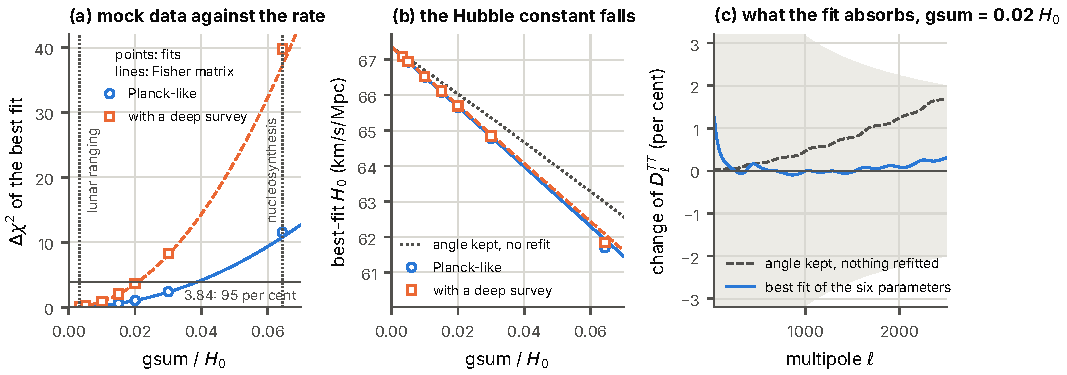
\includegraphics[width=\textwidth]{fig_forecast}
\caption{\label{fig:forecast}Mock data of the microwave background against the rate of deflation.
(a) The minimum $\Delta\chi^{2}$ of fits of the six parameters of the standard model at a fixed rate
(symbols) and the parabola of the Fisher matrix (lines), for the two data sets; the rates that lunar
laser ranging and nucleosynthesis allow are marked. (b) The best-fit Hubble constant, with the slope
of the Fisher matrix and, dotted, the Hubble constant that keeps the angle when nothing else is
refitted. (c) The temperature spectrum at $\gsum=0.02\,H_0$ relative to the data: with the angle kept
and nothing refitted, and at the best fit, which absorbs most of the difference; the band is the
cosmic variance of a single multipole.}
\end{figure*}

\emph{Deflation and dark radiation together.} The earlier paper fitted seven one-parameter families
of extra radiation to the same mock data: free-streaming radiation, a fluid, the stepped fluid of
the model at four transition redshifts $z_t$, and the Wess--Zumino stepped fluid, each with a
density $N$ in units of one neutrino species \cite{Flat1671}. Every family can raise
the Hubble constant, and every one at a price in $\Delta\chi^{2}$. Does the deflation lower the
price? We repeated all fits on the deflating spacetime at the largest rate that lunar laser ranging
allows, and computed the Fisher matrix with $N$ and the rate free together
(Table~\ref{tab:families}, Fig.~\ref{fig:families}). Three results follow.

First, at that rate every best-fit Hubble constant of the earlier paper falls by 0.274 to
$0.279~\kmsMpc$, which is the shift of the model without extra radiation: the effects of the
deflation and of the extra radiation add [Fig.~\ref{fig:families}(a), (b)].

Second, $N$ and the rate are positively correlated, with correlation coefficients of 0.37 to 0.89.
Extra radiation makes the early universe expand faster, the weaker gravity of the deflating
spacetime makes it expand more slowly, and in the spectra the two compensate in part. Fits with
extra radiation are therefore slightly \emph{better} on the deflating spacetime than on the static
one, slightly more extra radiation is allowed at a given $\Delta\chi^{2}$, and with both parameters
free the error of each grows, for free-streaming radiation from 0.143 to 0.250 in $N$.

Third, the compensation does not help the Hubble constant. When the rate grows and $N$ follows its
best-fitting value, the best-fit Hubble constant still falls: by $35.3~\kmsMpc$ per unit of
$\gsum/H_0$ for free-streaming radiation, against 84.35 without extra radiation, and by 22.1 to 76.9
for the seven families. The largest Hubble constant among the models with $N\ge0$, $\gsum\ge0$ and
$\Delta\chi^{2}\le3.84$ is therefore reached at zero rate, for every family and both data sets
[Fig.~\ref{fig:families}(c)]. \emph{The deflation lowers the Hubble constant faster than it makes
room for extra radiation.}

\begin{table*}
\caption{\label{tab:families}The dark-radiation families of the earlier paper on the deflating
spacetime (Planck-like mock data; assumptions A1, A2, A3). ``Model fluid'' is the stepped fluid of
the model with the transition redshift $z_t$. Columns 2 to 5: the density $N$ of extra
radiation at which the best fit reaches $\Delta\chi^{2}=4$, and the Hubble constant there in
$\kmsMpc$, with static extra coordinates (the earlier paper) and deflating at the largest rate that
lunar laser ranging allows. Columns 6 to 10, from the Fisher matrix with $N$ and the rate free together: the standard
error of $N$ with the rate held at zero and with the rate free; the correlation coefficient of $N$
and the rate; the net slope, that is, the change of the best-fit Hubble constant in $\kmsMpc$ per
unit of $\gsum/H_0$ when $N$ follows its best-fitting value; and the largest rise of the best-fit
Hubble constant, in $\kmsMpc$, among the models with $N\ge0$, $\gsum\ge0$ and
$\Delta\chi^{2}\le3.84$, which is reached at zero rate for every family.}
\begin{ruledtabular}
\begin{tabular}{lccccccccc}
 & \multicolumn{2}{c}{$N$ at $\Delta\chi^{2}=4$} & \multicolumn{2}{c}{$H_0$ there} & \multicolumn{2}{c}{error of $N$} & & net & largest \\
family & static & deflating & static & deflating & rate zero & rate free & correlation & slope & rise \\
\hline
free-streaming radiation & 0.29 & 0.31 & 69.74 & 69.62 & 0.143 & 0.250 & 0.82 & $-35.3$ & 2.30 \\
fluid, no step & 0.27 & 0.29 & 70.20 & 70.12 & 0.135 & 0.249 & 0.84 & $-23.9$ & 2.77 \\
model fluid, $z_t=10^4$ & 0.25 & 0.26 & 68.75 & 68.53 & 0.122 & 0.145 & 0.54 & $-65.4$ & 1.35 \\
model fluid, $z_t=2\times10^4$ & 0.17 & 0.18 & 68.16 & 67.90 & 0.085 & 0.091 & 0.37 & $-76.9$ & 0.78 \\
model fluid, $z_t=5\times10^4$ & 0.12 & 0.13 & 68.48 & 68.27 & 0.060 & 0.076 & 0.61 & $-67.0$ & 1.10 \\
Wess-Zumino fluid, $z_t=2\times10^4$ & 0.32 & 0.35 & 70.13 & 70.06 & 0.160 & 0.350 & 0.89 & $-22.1$ & 2.69 \\
model fluid, $z_t=10^6$ & 0.30 & 0.32 & 70.39 & 70.32 & 0.150 & 0.250 & 0.80 & $-23.0$ & 2.95 \\
\end{tabular}
\end{ruledtabular}
\end{table*}

\begin{figure*}
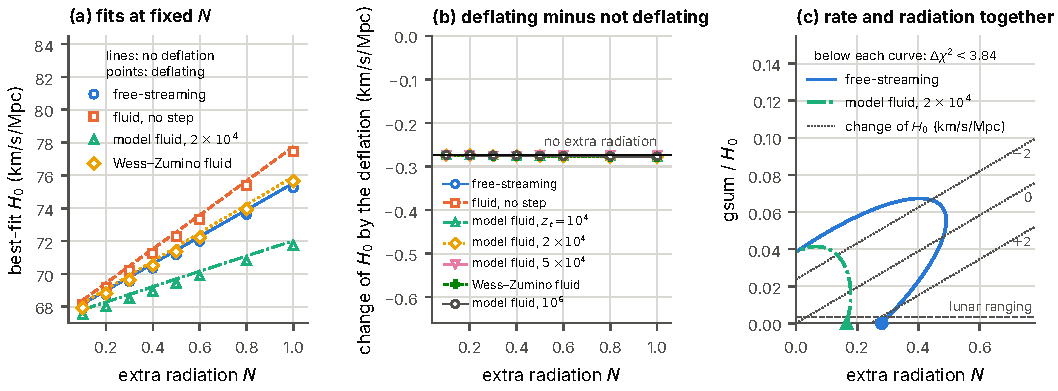
\includegraphics[width=\textwidth]{fig_families}
\caption{\label{fig:families}The dark-radiation families of the earlier paper on the deflating
spacetime (Planck-like mock data). (a) The best-fit Hubble constant against the density $N$ of extra
radiation for four families: without deflation (lines) and at the largest rate that lunar laser
ranging allows (symbols). (b) The difference for all seven families; the horizontal line is the
shift of the model without extra radiation. (c) The rate and the extra radiation as free parameters
together: the regions with $\Delta\chi^{2}<3.84$ of the Fisher matrix for two families, lines of
constant change of the best-fit Hubble constant for free-streaming radiation (dotted), the point of
the largest Hubble constant of each region (filled symbols, at zero rate), and the rate that lunar
laser ranging allows (dashed).}
\end{figure*}

\subsection{Dark matter}
\label{sec:dm}

\emph{What does not change.} The estimates of the earlier paper that decide whether the particles of
the model can be degenerate or condensed in observed halos contain the masses, the densities and the
velocities only, and the masses do not change along the deflation. Computed again, every number
agrees: fermions with eight internal states are degenerate in the core of a dwarf galaxy only if
they are lighter than 0.276~keV, and bound pairs are condensed there only if they are lighter than
262~eV. The verdict of the earlier paper on these two possibilities stands.

\emph{Self-interaction, and the epoch of the resonance.} The cross-section per mass of bound pairs
must respect the bound of about $1~\mathrm{cm^{2}/g}$ from colliding clusters
\cite{Markevitch2004,Randall2008}, which the earlier paper turned into a smallest allowed fermion
mass: 918~MeV for $\aVS=0.1$. For a given particle the masses are constant and so is this
cross-section. What the deflation changes is whether the pair \emph{exists}: it is bound only after
$\DVS$ has grown to $D_c$. And at that moment the scattering length of two unbound fermions
diverges (Sec.~\ref{sec:pair}), so that their cross-section rises to the limit that unitarity
allows, which is larger the slower the particles. For the example particle, $m=918$~MeV and
$m_s=54.7$~MeV, at the relative velocities 10, 156 and 1000~km/s [Fig.~\ref{fig:binding}(c)]: one
unit of the clock before the binding the cross-section per mass is $0.84~\mathrm{cm^{2}/g}$ at all
three velocities; at the binding it peaks at $1.3\times10^{7}$, $5.2\times10^{4}$ and
$1.3\times10^{3}~\mathrm{cm^{2}/g}$; and it exceeds $100~\mathrm{cm^{2}/g}$ during an interval of the
clock of 0.27, 0.27 and 0.26 around the binding. \emph{A deflating universe whose dark matter
consists of these fermions passes through an epoch of strong, velocity-dependent self-interaction},
strongest in the smallest halos. Whether the epoch lies in the observable past depends on the rate.
Under A2 and a constant rate it does so only if $\DVS$ today exceeds $D_c$ by less than a third of a
per cent, a coincidence that nothing in the model explains.

\emph{Superfluid dark matter and small-scale structure.} The earlier paper also asked what becomes
of the growth of structure if the dark matter is the superfluid itself, a fluid with first sound, in
two limits: a degenerate gas of the fermions with eight internal states, and a condensate of bound
pairs with the sound speed $c_{s0}$ today. The pressure of such a fluid suppresses structure below a
wavenumber, and the bound of the Lyman-$\alpha$ forest on warm dark matter
\cite{Viel2005,Irsic2017} then limits the fermion mass from below and the sound speed from above.
Computed again on the deflating background under A1 to A3, at the Hubble constant that keeps the
angle, the wavenumber at which the power falls to a quarter of that of cold dark matter is lower by
0.15 to 0.16 per cent at the rate that lunar laser ranging allows and by 3.0 to 3.3 per cent at the
rate that nucleosynthesis allows, for fifteen models. The reason is the weaker gravity of the time
at which the suppression is set: the Jeans wavenumber is proportional to the square root of Newton's
constant. The limits move accordingly, from $m>1.514$~keV and $c_{s0}<1.645\times10^{-11}\,c$ without
deflation to $m>1.516$~keV and $c_{s0}<1.641\times10^{-11}\,c$ at the first rate and $m>1.555$~keV
and $c_{s0}<1.565\times10^{-11}\,c$ at the second. The two closures give the same wavenumbers to
$1.5\times10^{-5}$. In this calculation the equation of state of the superfluid in ordinary space is
that of the earlier paper; whether the self-interaction of a condensate would itself follow the
volume of the deflating coordinates is a question about the microscopic model that the calculation
does not answer.

\emph{How fast the quantities drift.} With $n=d\ln(\text{quantity})/d\td$, the relative change of a
quantity over the age of the universe is $n\,\gsum\,t_0$. The couplings themselves drift with $n=1$
or $\tfrac12$ (Table~\ref{tab:exponents}). Quantities near a threshold drift much faster: the
scattering length just below the binding, at $\DVS=1.5$, with $n=9.1$; the binding energy just above
it, at $\DVS=1.8$, with $n=30$; the gap of a weakly paired state with $n=1/\lambda$. These are the
quantities in which a slow deflation would first be seen.

\subsection{The quanta that the deflation creates}

The temperature (\ref{eq:Tdefl}) of the quanta that the deflation creates in modes that depend on a
deflating coordinate is, for three equal rates at the bound of lunar laser ranging,
$2.9\times10^{-33}$~K. The number of created particles of mass $m$ per mode is $e^{-2\pi m/\rt}$, with an
exponent above $10^{37}$ for every mass above 1~keV at any rate allowed today. \emph{No particle is
created today.} Creation by deflation matters only for an epoch in which the rate was comparable
with the masses, which no bound of this section addresses.

\subsection{Verdict on hypothesis H3}

\emph{The Hubble tension.} The mechanism of the earlier paper, the phase mode of the Vorton-Scalar
as dark radiation, is untouched at the allowed rates, since the couplings drift by parts in a
thousand; its verdict stands and is not improved. The deflation itself contributes two effects. The
first, through Newton's constant, has the wrong sign: at a fixed angle of the sound horizon the
inferred Hubble constant falls by $0.2~\kmsMpc$ at the largest rate that lunar laser ranging allows,
and in fits to mock data of the microwave background it falls by $84~\kmsMpc$ per unit of
$\gsum/H_0$. Nor can the rate help the dark radiation: more extra radiation is allowed when the rate
is free, but the largest Hubble constant that the mock data allow is reached at zero rate. The
second effect, the loss of mass of bound pairs, has the right sign and is bounded, in the examples
computed, to $0.5~\kmsMpc$. \emph{The hypothesis that the model resolves the Hubble tension is not
supported by the deflation, and under A2 it is mildly disfavored.}

\emph{Dark matter.} The conclusions of the earlier paper about the mass ranges hold unchanged, and
its limits on superfluid dark matter move by two tenths of a per cent at the rate that lunar laser
ranging allows. The deflation adds one qualitative prediction, the epoch of the resonance, and one
quantitative one, a rise of the growth rate, whose size depends on the perturbations of the agent.
Neither is in conflict with observation at the allowed rates, and neither is detectable at the rate
that lunar laser ranging allows. \emph{The hypothesis that the superfluid is the dark matter is
neither strengthened nor weakened by the deflation.} It acquires a history, whose observable part is
empty if gravity is eight-dimensional and the rate constant.

\emph{What rests on the additional assumptions.} Everything in this section that concerns Newton's
constant rests on A2. The spectra, the forecast and the growth of structure rest in addition on A3,
and the growth of structure and the largest angular scales on a closure that the hypothesis of
deflation does not supply. The forecasts are for mock data without gravitational lensing; no
measured spectrum has been fitted.

\section{The Higgs hypothesis}
\label{sec:higgs}

\subsection{The hypothesis and the conditions}

Hypothesis H2 says that the superfluid state, the condensate of the fermion pair along the hidden
axis, \emph{is the Higgs field} \cite{Higgs1964}. In the Standard Model the Higgs field is a doublet
of the weak-isospin group with a vacuum value $\vEW=246$~GeV, which breaks the electroweak symmetry,
gives the W and Z bosons and the quarks and charged leptons their masses, and leaves one scalar
particle of 125~GeV. Its four real components form a vector of a group $SO(4)$, which the vacuum
value breaks to $SO(3)$ \cite{Sikivie1980}. The earlier paper derived from this seven conditions that
a condensate must meet in order to \emph{be} the Higgs field (Table~\ref{tab:conditions}) and found
the hypothesis unproven
on the flat $7{+}1$ spacetime, with one structural point in its favor: the order parameter has the
representation and the breaking pattern of the Higgs field under a symmetry of the spacetime. This
section repeats the test on the deflating spacetime.

Two statements must be kept apart. H2 is the hypothesis that the \emph{pair condensate} is the Higgs
field; the electroweak scale is then the scale of the condensate. HV, used in one row of
Table~\ref{tab:bounds}, is the different assumption that the vacuum value of the
\emph{Vorton-Scalar} sets the electroweak scale. HV is not examined here.

\begin{table*}
\caption{\label{tab:conditions}The conditions that a condensate must meet in order to be the Higgs
field, and their status on the deflating $7{+}1$ spacetime. The last row is new.}
\begin{ruledtabular}
\begin{tabular}{p{0.32\textwidth}p{0.62\textwidth}}
condition & status \\
\hline
C1: a scalar under the Lorentz group of ordinary spacetime & met in the sector of fields that do not depend on the extra coordinates \\
C2: non-zero in empty space & open; reached by the deflation only outside the range of validity of the model \\
C3: a doublet of the weak-isospin group with a neutral component & only under a hidden symmetry (three different rates), or with $SO(3)$ alone as a symmetry of the spacetime (equal rates) \\
C4: breaks $SO(4)$ to $SO(3)$ & met in the sector; the spacetime itself has at most the $SO(3)$ \\
C5: scale 246~GeV, with a scalar particle of 125~GeV with the observed couplings & unfavorable (estimate of the earlier paper, unchanged) \\
C6: its couplings give the quarks and leptons their masses & not addressed \\
C7: no further light or charged particles that would have been seen & additional particles are predicted \\
new: the electroweak scale does not drift & requires $\gsum<1.16\times10^{-6}\,H_0/\nEW$ \\
\end{tabular}
\end{ruledtabular}
\end{table*}

\subsection{What the deflation leaves unchanged}

The pair operators, their transformation properties and the internal symmetry are properties of the
Dirac matrices of the frame, which the deflation does not change, and of the equations of the fields
that do not depend on the extra coordinates, which for the weighted fields are the flat equations.
By Sec.~\ref{sec:hidden} the four vector pair operators form the $(2,2)$ of
$SU(2)_A\times SU(2)_B$, the representation of a Higgs field, and a condensate along one axis breaks
$SO(4)$ to $SO(3)$. Hence, \emph{within the sector}, C1 holds as on flat spacetime: the pair along
the hidden axis is invariant under the rotations of $x1,x2,x3$, which remain symmetries of the
spacetime, and under the boosts of ordinary spacetime as they act on the fields of the sector. (The
boosts are no longer symmetries of the deflating spacetime as a whole; in the sector this shows only
in the dependence of the couplings on the time.) C3 and C4 hold in the sector as well, in the sense
that the pattern is right under its internal symmetry.

\subsection{What the deflation changes}

On the flat $7{+}1$ spacetime the six generators of $SO(4)$ are rotations of the extra dimensions. This
is what the earlier paper counted in favor of the hypothesis: a symmetry of extra dimensions is the
kind of symmetry from which a gauge interaction can arise, as in the theories of Kaluza and Klein
\cite{Witten1981}. By Sec.~\ref{sec:hidden} the deflating spacetime keeps none, one or three of the
six, and never one of the three that mix the hidden axis with a deflating coordinate.

For equal rates the part of $SO(4)$ that remains a symmetry of the \emph{spacetime} is $SO(3)$, the
rotations of the three deflating coordinates: precisely the subgroup that a condensate along $x0$
would leave unbroken.
The deflation thus breaks $SO(4)$ to $SO(3)$ \emph{explicitly}, at the level of the geometry, in
the same pattern in which the hypothesis needs the condensate to break it \emph{spontaneously}.
Three consequences follow. First, the three broken generators, which under H2 would correspond to
the massive weak bosons, are not symmetries of the spacetime at all; a gauge interaction for them
cannot arise from the geometry of the deflating spacetime. Second, in the sector the full $SO(4)$
nevertheless acts as an exact symmetry, but as a hidden one. The companion paper finds exactly this
situation on the $4{+}4$ spacetime, flat or deflating, where the hypothesis has no geometric basis
\cite{CompanionDefl1644}. \emph{The deflation puts the $7{+}1$ model in the position of the $4{+}4$
model.} Third, the potential of the order parameter does not single out the hidden axis
(Sec.~\ref{sec:order}): within the sector the direction of the condensate is as free as on flat
spacetime. Outside the sector the axes differ, because a variation of the order parameter along a
deflating coordinate costs a gradient energy that grows as $1/b_t^{2}$; the hidden symmetry is exact
only for fields that are strictly independent of the extra coordinates.

\subsection{Condition C2: a condensate in empty space}

The earlier paper left C2 open: a pair condensate forms in the vacuum only if $\aVS$ exceeds a
critical value $\alpha_c$ of about 2 or more, depending on the cutoff. On a deflating spacetime
$\aVS$ grows as $e^{\td}$ and reaches any such value at a definite time. Section~\ref{sec:cjt} showed
what else has happened by then: the exchange of one boson is no longer a controlled approximation,
and the field at which the one-loop potential of the Vorton-Scalar falls below its vacuum value has
moved to within a factor of two of the vacuum value. \emph{C2 can be reached by waiting, but not
within the range of validity of the model.} Its status remains open.

\subsection{A new condition: the electroweak scale must not drift}

Suppose that H2 holds. The electroweak scale $\vEW$ is then the scale of the pair condensate in the
vacuum, as in models in which a condensate of fermions replaces the elementary Higgs field
\cite{BardeenHillLindner1990}. That scale is determined by the parameters of the model: the masses
$m$ and $m_s$, the cutoff, and the coupling $\aVS$. On the deflating spacetime the masses are constant
and $\aVS\propto e^{\td}$. Therefore
\begin{equation}
\vEW\ \propto\ e^{\,\nEW\,\td},\qquad\nEW=\frac{d\ln\vEW}{d\ln\aVS}.
\label{eq:nEW}
\end{equation}
The exponent cannot vanish: below the critical coupling there is no condensate, so that the scale
depends on the coupling, and most strongly just above the critical coupling.

Under H2 the masses of the electron and of the quarks are proportional to $\vEW$ and change at the
rate $\nEW\,\gsum$. The mass of the proton is due mostly to the strong interaction and does not
follow. The ratio $m_p/m_e$ of the proton mass to the electron mass therefore changes at the rate
$\nEW\,\gsum$. Comparisons of atomic clocks find this ratio constant to $8.0\times10^{-17}$ per year
at two standard deviations \cite{Lange2021}. Hence
\begin{equation}
\gsum<\frac{8.0\times10^{-17}\ \text{per year}}{\nEW}=\frac{1.16\times10^{-6}\,H_0}{\nEW}.
\label{eq:clockbound}
\end{equation}
The bound needs no assumption about gravity. For $\nEW=1$ it is 2787 times stronger than the bound
that lunar laser ranging gives if gravity is eight-dimensional.

\emph{The size of the exponent.} For the model itself, with massive fermions and a massive radial
mode, the scale of the vacuum condensate has not been computed as a function of the coupling. It is
known in closed form for the case on which the earlier paper tested its ladder equation: massless
fermions and massless bosons between an infrared scale and a cutoff \cite{Miransky1985}. There the
scale of the condensate obeys
\begin{equation}
\varrho_c\,\ln\frac{\text{cutoff}}{\text{scale}}=\arctan\frac{1}{2\varrho_c},\qquad
\varrho_c^{2}=\frac14\Big(\frac{\aVS}{\alpha_c}-1\Big),
\end{equation}
where $\varrho_c$ is only an abbreviation for the square root that the second equation defines, from
which
\begin{equation}
\nEW=\frac{(1+4\varrho_c^{2})\,\arctan(1/2\varrho_c)}{8\,\varrho_c^{3}}+\frac{1}{4\varrho_c^{2}}.
\label{eq:nEWladder}
\end{equation}
The program verifies Eq.~(\ref{eq:nEWladder}) against the numerical derivative to $3\times10^{-8}$
and tabulates it with the bound (\ref{eq:clockbound}) (Table~\ref{tab:higgs}). The exponent diverges
at the critical coupling, equals $1+\pi/2=2.57$ at twice the critical coupling, and exceeds 1 for
$\aVS<3.27\,\alpha_c$. It falls below 1 only where the scale of the condensate approaches the cutoff,
that is, where the four-dimensional description ends. Within the range in which a condensate of the
kind that H2 needs can be described at all, $\nEW$ is of order one or larger.

\begin{table}
\caption{\label{tab:higgs}The exponent $\nEW$ with which the scale of the vacuum condensate follows
the coupling in the scale-invariant ladder equation, and the bound (\ref{eq:clockbound}) on the
present rate of deflation that follows from it under hypothesis H2.}
\begin{ruledtabular}
\begin{tabular}{ccccc}
$\aVS/\alpha_c$ & $\ln$(cutoff/scale) & $\nEW$ & $\gsum$ (per year) & $\gsum/H_0$ \\
\hline
1.05 & 12.082 & 147 & $5.4\times10^{-19}$ & $7.9\times10^{-9}$ \\
1.10 & 7.998 & 54.0 & $1.5\times10^{-18}$ & $2.2\times10^{-8}$ \\
1.25 & 4.429 & 15.1 & $5.3\times10^{-18}$ & $7.7\times10^{-8}$ \\
1.50 & 2.702 & 6.05 & $1.3\times10^{-17}$ & $1.9\times10^{-7}$ \\
2.00 & 1.571 & 2.57 & $3.1\times10^{-17}$ & $4.5\times10^{-7}$ \\
3.00 & 0.870 & 1.15 & $6.9\times10^{-17}$ & $1.0\times10^{-6}$ \\
5.00 & 0.464 & 0.540 & $1.5\times10^{-16}$ & $2.2\times10^{-6}$ \\
10.0 & 0.215 & 0.230 & $3.5\times10^{-16}$ & $5.0\times10^{-6}$ \\
\end{tabular}
\end{ruledtabular}
\end{table}

\emph{The conclusion.} Under H2 the deflation clock can have advanced by at most
$\gsum\,t_0<1.1\times10^{-6}/\nEW$ during the age of the universe at a constant rate. Every effect of
the deflation described in Secs.~\ref{sec:gap} to \ref{sec:cosmo} is then unobservably small.
Conversely, a deflation at any rate at which those effects matter excludes H2. \emph{The hypothesis
H2 and a deflation of any consequence today exclude each other.} This conclusion does not depend on
the unresolved conditions C2 and C5 to C7. It depends on two properties only: that the electroweak
scale is set by the dynamics of the model, which is the content of H2, and that the coupling of the
model follows the volume of the deflating coordinates, which is exact (Sec.~\ref{sec:clock}).

\subsection{Verdict on hypothesis H2}

On the deflating spacetime the hypothesis that the singlet superfluid is the Higgs field is
unproven, with less in
its favor than on the flat $7{+}1$ spacetime, and it is incompatible with any deflation that is fast
enough to matter today. Whether a mechanism exists that would make the electroweak scale insensitive
to the coupling of the pair is not known; none is present in the model.

\section{What has been established, and what has not}
\label{sec:status}

The sections above reported results of very different standing: identities verified in exact
arithmetic, numerical results with a stated accuracy, consequences of additional assumptions, and
estimates. This section sorts them. An item is called established if a machine check stands behind
it (Appendix~\ref{app:checks}); statements of interpretation deserve the reader's independent
scrutiny more than the numbers do.

\subsection{Established}

\emph{Geometry} (Sec.~\ref{sec:geometry}). The curvature and the Einstein tensor of the deflating
spacetime in closed form, for arbitrary rates and constants. The Killing vectors, 14, 15 or 20 in
number, and the completeness of the lists. That the spacetime is not a solution of Einstein's
equations without matter, with or without a cosmological constant; that with three equal rates it is
an exact solution of Einstein-Gauss-Bonnet gravity without matter, for $\Lam=3\,\gff^{2}$ and
$\aGB=-1/(4\,\gff^{2})$; and that with unequal rates it is not.
The unbounded blueshift of a classical particle that moves along a deflating coordinate, and
the incompleteness of its geodesic.

\emph{The Dirac field} (Secs.~\ref{sec:dirac}, \ref{sec:modes}). The Dirac matrices in coordinate
components, the spin connection, the covariant constancy of the matrices, and the curvature of the
spinor derivative. The Dirac equation, the weighted field, and the statement that fields which do
not depend on $x5,x6,x7$ obey the flat equation.
The exact solutions when one rate governs, and
the law of creation (\ref{eq:ncr}) with the temperature (\ref{eq:Tdefl}). All of this is confirmed
numerically by two independent methods.

\emph{The model along the clock} (Secs.~\ref{sec:clock} to \ref{sec:cjt}). For fields that do not
depend on the extra coordinates, the model of the earlier paper on the deflating spacetime is the
same model with the couplings of the moment, exactly. The masses are constant; $\gVS$ grows as
$e^{\td/2}$; $\aVS$, $\GVS$, $\DVS$ and $C$ grow as $e^{\td}$. The modes of the Vorton-Scalar grow
with the weight only, and the potential between two fermions has the unchanged range and the
strength of the moment. The exchange amplitudes are those of flat spacetime times the square of the
coupling of the moment. In weak coupling the gap grows according to Eq.~(\ref{eq:growth}), and the
critical temperature follows it. Two fermions become bound at a definite time, at a scattering
resonance, with a binding energy that starts quadratically; the order of the other events depends on
$m_s/m$ alone. The paired state follows the deflation if and only if $\Xid$ is below about 0.2 to
0.5; before that it lags and accumulates broken pairs. The solution of the gap equation is a minimum
of the effective potential at every moment examined. Matter of fixed density loses its fermion mass
at a critical value of $C$, is self-bound for $C>3.7011$ and is more strongly bound later; the
melting temperature of the fermion mass falls; the barrier of the one-loop potential of the vacuum
moves toward the vacuum value.

\emph{Order parameter and symmetry} (Sec.~\ref{sec:order}). The potential of the order parameter
prefers no direction among the four frame axes. The internal symmetry of the sector, the
representation of the pair operators and the breaking pattern are unchanged by the deflation. Of the
six generators that belong to the pairs of the four extra axes, the deflating spacetime keeps none,
one or three as symmetries of the spacetime. A vortex line of unit winding carries four fermion zero
modes, two for each direction along the line, at every moment; its energy per length falls as
$e^{-\td}$.

\emph{Cosmology} (Sec.~\ref{sec:cosmo}), each item under the assumption named there. The equation of
the expansion (\ref{eq:friedmann}) and the fall of the inferred Hubble constant, with recombination
computed on the deflating background and verified by an independent calculation. The bounds of
Table~\ref{tab:bounds}, and that in the model as it stands the atomic clocks give none. The effect
of the loss of mass of bound pairs. The pressure (\ref{eq:pagent}) of the agent. The equations
(\ref{eq:pert}) of the perturbations of ordinary space for unperturbed extra scale factors, the
identities (\ref{eq:id1}) and (\ref{eq:id2}), and that the four equations cannot all hold with matter
alone. The growth equations of the two closures, and that the closure ``Shear'' coincides with the
closure ``Pressure'' inside the horizon. The spectra of the microwave background for $\ell\ge30$ and
their independence of the closure; the forecast for the rate from mock data; that the Hubble
constant falls in every fit, with or without extra radiation; and that extra radiation and the rate
of deflation compensate in part in the spectra, without any gain for the Hubble constant. The
unchanged estimates of degeneracy
and of condensation in halos, the limits on superfluid dark matter, the epoch of the resonance, and
the drift of the quantities. The temperature of the created quanta at the allowed rates.

\emph{The Higgs hypothesis} (Sec.~\ref{sec:higgs}). Under H2 the electroweak scale follows the
coupling with the exponent $\nEW$, and atomic clocks bound the rate of deflation by
Eq.~(\ref{eq:clockbound}). The exponent is given in closed form for the scale-invariant ladder
equation.

\subsection{Not established}

\emph{The source of the deflation.} The metric is prescribed. For equal rates it solves the
equations of Einstein-Gauss-Bonnet gravity without matter; whether that solution is stable has not
been examined. For unequal rates no field equation has been found that the metric solves, and the
stress tensor that Einstein's equations would require has not been identified with any matter. All
results on fields are results on a given background.

\emph{The theory of gravity and the assumption A2.} If gravity is of the Einstein-Gauss-Bonnet kind,
the relation (\ref{eq:GN}) between Newton's constant and the volume of the deflating coordinates,
and with it every result of Sec.~\ref{sec:cosmo} that is marked A2, would have to be derived anew.

\emph{The agent.} Nothing in the hypothesis says what keeps the three rates constant while ordinary
space expands. Under A2 it must have the tension (\ref{eq:pagent}) and no energy density; whether a
physical source with these properties exists has not been examined. Nor does the hypothesis say how
the agent responds when ordinary space is perturbed. That the scale factors of the deflating
coordinates are not perturbed (assumption A3) is an assumption; and even with it, a closure is
needed that the hypothesis does not supply. The growth of structure, the amplitude $\sigma_8$ and
the spectra of the microwave background at the largest angular scales are computed for two closures
and differ between them at the first order in the rate. They are the quantities that a theory of
the agent would have to predict.

\emph{The reaction of the created particles on the metric.} The particles created by the deflation
gain energy without bound. Their stress must eventually change the metric; this has not been
computed. Nor do the coordinates cover the whole future of particles that move along deflating
coordinates; what lies beyond is outside the hypothesis.

\emph{The restriction to the sector.} That the fields do not depend on $x5,x6,x7$ is assumed, as in
the earlier paper. The deflation supports the assumption only if the deflating coordinates are
periodic (Sec.~\ref{sec:modes}).

\emph{Unequal rates with simultaneous crossings.} No closed form is known for a mode that depends on
two deflating coordinates whose crossings coincide; the results are numerical.

\emph{The hidden coordinate.} That the fields do not depend on $x0$ is assumed, as in the earlier
paper. Nothing in the deflation explains it.

\emph{The end of the history.} The couplings grow without bound. The four-dimensional description
with the exchange of one boson holds only while $\aVS$ is not large, and the eight-dimensional theory
itself is an effective theory, with couplings of negative mass dimension, that must fail when the
proper size of the deflating coordinates reaches its scale of validity. What happens then is outside
the model. Every history of Secs.~\ref{sec:gap} to \ref{sec:cjt} ends in a regime that the two-loop
truncation does not control; the numbers at the last moments of each table indicate the trend and
are not predictions.

\emph{The energy.} The energy of matter is not conserved while the couplings change. Where it goes,
into whatever drives the deflation, is not described.

\emph{Dynamics.} Sections~\ref{sec:gap}, \ref{sec:pair} and \ref{sec:cjt} give sequences of
equilibrium states. Only for the paired state has the ability to follow been examined, in a model
without dissipation; with dissipation the broken pairs would relax, and their lifetime is not known.
The time-dependent two-body problem at the moment of binding, which decides how much of the
population ends in the bound state, has not been solved. How a gas reaches the self-bound state, and
whether the abnormal state forms by nucleation, are open. The equilibrium of a loop of vortex line
with its current, and its stability, have not been computed.

\emph{The vacuum beyond one loop.} The statements about the vacuum use the one-loop potential
outside its range of reliability and draw only the conclusion stated in Sec.~\ref{sec:cjt}.

\emph{Cosmology.} The forecasts of Sec.~\ref{sec:forecast} are for mock data without gravitational
lensing; no measured spectrum of the microwave background has been fitted. All bounds that reach
back to nucleosynthesis or to recombination assume a constant rate; a rate that was large early and
is small today is neither excluded nor described. Only linear perturbations were computed. The
consequences of the epoch of the resonance for the formation of halos have not been simulated.

\emph{The Higgs hypothesis.} Everything that the earlier paper lists as not established: that a
condensate forms in the vacuum, that the rotation group of the extra
dimensions is the electroweak gauge group, the scale and the mass of the scalar particle, and the
masses of ordinary fermions. The exponent $\nEW$ has not been computed for the model itself; the
statement that it is of order one or larger rests on the scale-invariant case and on the general
fact that the scale of the condensate vanishes at the critical coupling.

\section{Conclusions}
\label{sec:concl}

We asked what becomes of a 16-component Dirac field, and of the superfluid of its pairs, when three
of the eight coordinates of a spacetime of signature $7{+}1$ deflate exponentially.

The geometry is simple and rigid. The deflating spacetime is homogeneous, it has 14 to 20 symmetries
instead of 36, and it is not a solution of Einstein's equations without matter. With three equal
rates it is an exact solution of Einstein-Gauss-Bonnet gravity without matter, for one relation
between the rate and the two constants of that theory.

The Dirac field separates into two parts. Fields that do not depend on the deflating coordinates
obey, after a change of normalization, exactly the flat equations.
Fields that do depend on them are populated by the deflation with a
Fermi-Dirac spectrum at the temperature of the rate divided by $2\pi$, and their quanta then gain
energy without bound.

The superfluid of hypothesis H1 exists on the deflating spacetime at every moment, with the
couplings of that moment, and it acquires a history. The masses do not change; the coupling grows
with the inverse volume of the deflating coordinates; the gap grows much faster than the coupling,
in weak coupling as the exponential of an exponential; two fermions become bound at a scattering
resonance; matter loses its fermion mass and
becomes self-bound; and the paired state can follow the deflation only once its gap exceeds a few
times the rate divided by the pairing strength. The direction of the order parameter is not selected
by the deflation.

For hypotheses H2 and H3 the deflation brings no relief. The rotations that gave the Higgs hypothesis
its one structural support on the flat $7{+}1$ spacetime are no longer symmetries of the spacetime.
If the superfluid were the Higgs field, the electroweak scale would follow the growing coupling, and
atomic clocks would then limit the rate of deflation to about a millionth of the Hubble rate. If
gravity is the Einstein theory in eight dimensions, lunar laser ranging limits it to three
thousandths of the Hubble rate, and the Hubble constant inferred from the microwave background
moves away from the local measurement, in the simplest estimate and in fits of all parameters to
mock data alike. In either case nothing of the history just described can have happened within the
age of the universe at a constant rate.

The perturbations of ordinary space show most plainly what the hypothesis of deflation leaves open.
Whatever keeps the rates constant must carry a tension, and it must take part in the perturbations:
with a Newton's constant that depends on the time, the Einstein equations of ordinary space cannot
all hold with matter alone. The spectra of the microwave background at all but the largest angular
scales do not depend on how the agent does so, and mock data of the quality of the Planck satellite
would bound the rate to four per cent of the Hubble rate. The growth of structure does depend on it,
at the first order in the rate.

These results are quantitative, and they come with the programs that produced them. They mark what
a successful theory of this kind would have to supply: a source or a theory of gravity that sustains
the deflation and that says how the source responds to perturbations, a rate that was large early
and is small today, and a reason why the constants of ordinary matter do not follow the volume of
the deflating coordinates.

\section*{Data availability}

The source code of all programs, the data files from which every figure and every computed number of
this paper is generated, the instructions for compiling and running the programs, the supplements
that derive each result step by step, and the documents that record the provenance of each result
are openly available \cite{DeflationRepo}.

\appendix

\section{Symbols}
\label{app:symbols}

Tables~\ref{tab:symbols}, \ref{tab:symbols2} and \ref{tab:symbols3} list the symbols of this paper
with the place of their definition. Symbols of the earlier paper \cite{Flat1671} keep their meanings. The complete registry, with
the machine checks that no symbol has two meanings, is part of Ref.~\cite{DeflationRepo}.

\begin{table*}
\caption{\label{tab:symbols}The symbols of this paper: geometry and the Dirac field.}
\begin{ruledtabular}
\begin{tabular}{p{0.2\textwidth}p{0.6\textwidth}p{0.14\textwidth}}
symbol & meaning & defined in \\
\hline
$x0,\dots,x7$ & the eight coordinates: $x0$ hidden space-like coordinate; $x1,x2,x3$ ordinary space; $x4$ ordinary time; $x5,x6,x7$ the deflating coordinates, space-like & Sec.~\ref{sec:intro} \\
$xt$; $xj$; $a$ & a deflating coordinate, $t\in\{5,6,7\}$; a flat coordinate other than the time, $j\in\{0,1,2,3\}$; index of the four extra axes, $a\in\{0,5,6,7\}$ & Sec.~\ref{sec:intro} \\
$\gff$, $\gss$, $\gvv$; $\rt$ & the three rates of deflation (upright, without subscript; not components of the metric); the rate of $xt$ & Eq.~(\ref{eq:hyp}) \\
$\cff$, $\css$, $\cvv$; $\ct$ & the three positive constants of the metric: the scale factors at $x4=0$ & Eq.~(\ref{eq:hyp}) \\
$\gsum$, $\gsq$, $\gprod$ & the sum of the rates, the sum of their squares, the sum of their products in pairs & Sec.~\ref{sec:geometry} \\
$b_t$ & scale factor of the deflating coordinate $xt$ & Eq.~(\ref{eq:scale}) \\
$\eta$; $g_{\mu\nu}$; $e_A{}^{\mu}$ & flat metric; metric of the deflating spacetime; orthonormal frame & Eq.~(\ref{eq:metric}) \\
$\Vd$ & proper volume of a unit coordinate cell of the deflating coordinates & Eq.~(\ref{eq:Vd}) \\
$\Gamma^{\rho}{}_{\mu\nu}$; $R^{\rho}{}_{\sigma\mu\nu}$, $R^{\mu}{}_{\nu}$, $R$ & Christoffel symbols; Riemann tensor [in Eq.~(\ref{eq:riemann}) its components in the orthonormal frame], Ricci tensor, curvature scalar & Sec.~\ref{sec:curvature} \\
$\cG^{\mu}{}_{\nu}$; $\cH^{\mu}{}_{\nu}$; $\Lam$, $\aGB$ & Einstein tensor; Lanczos tensor of the Gauss-Bonnet term; cosmological constant and coupling of Einstein-Gauss-Bonnet gravity & Sec.~\ref{sec:egb} \\
$\cX_{\mathrm{scale}}$, $\cX_{(s)}$ & the scaling Killing vector; the three special Killing vectors of the case of equal rates & Eqs.~(\ref{eq:scaling}), (\ref{eq:special}) \\
$K_{AB}$; $\bar x4$, $\bar xt$ & sectional curvature of the plane of the frame directions $A$ and $B$; coordinates adapted to the case of equal rates & Appendix~\ref{app:curvature} \\
$P_\mu$; $\varsigma$ & conserved momenta of a classical particle; affine parameter & Sec.~\ref{sec:geodesics} \\
$\gamma^{A}$, $\gamma^{\mu}$; $\Omega_\mu$, $\omega_{\mu AB}$ & Dirac matrices of the frame and in coordinate components; spin connection and its coefficients & Sec.~\ref{sec:dirac} \\
$\chi$, $P^{L,R}$; $\Cm$ & chirality matrix and the two chiral projectors; the matrix that turns each Dirac matrix into minus its transpose & Secs.~\ref{sec:clock}, \ref{sec:gap} \\
$\psi_{\tg}$; $\hpsi$ & the 16-component field on the deflating spacetime; the weighted field $\sqrt{\Vd}\,\psi$ & Eqs.~(\ref{eq:dirac}), (\ref{eq:weighted}) \\
$\hh$, $\hh_\perp$; $\beta$, $\alpha^{A}$, $\alpha^{d}$; $\bar\psi$ & Hamiltonian of a mode, and its part without the scale factors; $\gamma^{4}$, $\gamma^{4}\gamma^{A}$, and the matrix $\alpha$ along the wave vector in the deflating coordinates; the adjoint $\psi^\dagger\beta$ & Eqs.~(\ref{eq:h}), (\ref{eq:LVS}) \\
$p_j$, $k_t$; $\Eperp$; $\kd$; $\ud$ & wavenumbers along the flat and the deflating coordinates; $(m^{2}+\sum_jp_j^{2})^{1/2}$; physical wavenumber along the deflating coordinates; $\kd/\rt$ & Eqs.~(\ref{eq:kd}), (\ref{eq:ud}) \\
$w$; $Z_+$, $Z_-$ & one of the eight constant spinors from which the exact solutions are built; two cylinder functions whose orders differ by one & Eq.~(\ref{eq:exact}) \\
$\ncr$; $\Tdefl$ & number of quanta that the deflation creates in a mode, per internal state; temperature of their spectrum & Eqs.~(\ref{eq:ncr}), (\ref{eq:Tdefl}) \\
\end{tabular}
\end{ruledtabular}
\end{table*}

\begin{table*}
\caption{\label{tab:symbols2}The symbols of this paper, continued: the model and the superfluid.}
\begin{ruledtabular}
\begin{tabular}{p{0.2\textwidth}p{0.6\textwidth}p{0.14\textwidth}}
symbol & meaning & defined in \\
\hline
$\mathcal L_{\tg}^{\mathrm{VS}}$; $\PhiVS$, $\hat\Phi_{\mathrm{VS}}$ & Lagrangian of the model; the Vorton-Scalar and its weighted form $\sqrt{\Vd}\,\PhiVS$ & Eq.~(\ref{eq:LVS}) \\
$\lamVS$, $\vVS$, $\yVS$ & self-coupling of the Vorton-Scalar, the constant that fixes its vacuum value, its Yukawa coupling & Sec.~\ref{sec:clock} \\
$U(1)_F$, $\UVS$; $\epsilon$ & the symmetries of fermion number and of chirality; parameter of a symmetry transformation & Sec.~\ref{sec:clock} \\
$m$, $m_s$; $\gVS$, $\aVS$ & fermion mass, mass of the radial mode; coupling of both modes to the fermions, and $\gVS^{2}/4\pi$ & Eq.~(\ref{eq:masses}) \\
$\DVS$, $C$; $D_c$ & the two numbers that decide the state of matter; critical value of $\DVS$ for a bound pair & Eq.~(\ref{eq:DC}) \\
$\td$; $\tpair$ & the deflation clock; the clock measured from the binding of the pair & Eqs.~(\ref{eq:clock}), (\ref{eq:tpair}) \\
$\varphi_{\mathrm{bos}}$, $m_{\mathrm{bos}}$, $\varpi_b$ & a mode of the Vorton-Scalar, its mass, the frequency of its weighted form & Sec.~\ref{sec:scalarmodes} \\
$F_S$, $F_P$; $W(k,k')$ & exchange amplitudes of the radial and of the phase mode; kernel of the gap equation (always written with its two arguments) & Sec.~\ref{sec:gap} \\
$\lambda$, $\lambda_S$, $\lambda_P$; $\Delta_F$; $T_c$ & pairing strength, and its parts from the radial and from the phase mode; gap at the Fermi momentum; critical temperature & Sec.~\ref{sec:gap} \\
$\kF$, $\EF$, $v_F$, $N(0)$ & Fermi momentum, Fermi kinetic energy, Fermi velocity, density of states at the Fermi surface per internal state & Secs.~\ref{sec:gap}, \ref{sec:cjt} \\
$a_{\mathrm{sc}}$, $E_b$ & scattering length of two fermions; binding energy of the pair & Sec.~\ref{sec:pair} \\
$\Xid$; $\Deq$; $\Esh$; $\nex$ & the parameter that decides whether the paired state follows the deflation; equilibrium gap; half-width of the shell of states; density of broken pairs & Sec.~\ref{sec:quench} \\
$\xi_k$, $E_k$, $\kappa$, $n_k$ & single-particle energy, quasi-particle energy, pair correlation and occupation of a pair of states & Eq.~(\ref{eq:bloch}) \\
$V[\Delta]$; $\phi$; $m^{*}$; $T_{1/2}$ & effective potential of the paired state; expectation value of the Vorton-Scalar; fermion mass in matter; temperature at which the fermions have lost half of their mass & Sec.~\ref{sec:cjt} \\
$\Delta^{a}$, $\Delta_t$; $\MM$; $d_\pm$ & order parameter (frame components), and its coordinate components along the deflating coordinates; gap matrix; the two fourfold gaps of a state & Sec.~\ref{sec:order} \\
$SU(2)_A$, $SU(2)_B$, $U(1)_E$ & the factors of the internal symmetry of the fields that do not depend on the extra coordinates & Sec.~\ref{sec:hidden} \\
$P$, $P_c$; $w_z$; $\theta_{12}$ & generator of $U(1)_E$ and the product of the five matrices of the sector; spinor of a zero mode; angle around a vortex line & Sec.~\ref{sec:vortex} \\
\end{tabular}
\end{ruledtabular}
\end{table*}

\begin{table*}
\caption{\label{tab:symbols3}The symbols of this paper, continued: the cosmological part and the
Higgs hypothesis.}
\begin{ruledtabular}
\begin{tabular}{p{0.2\textwidth}p{0.6\textwidth}p{0.14\textwidth}}
symbol & meaning & defined in \\
\hline
$a_{\mathrm{sp}}$, $H$, $H_0$; $\GN$, $G_8$ & scale factor of ordinary space, Hubble rate, Hubble constant; Newton's constant and the constant of gravitation in eight dimensions & Sec.~\ref{sec:cosmo} \\
$\rho$, $\rho_m$; $\omega_b$, $\omega_c$ & energy density in ordinary space, and that of matter; the densities of baryons and of cold dark matter of the standard model of cosmology & Sec.~\ref{sec:cosmo} \\
$\theta_*$, $r_s$; $t_0$; $z_*$, $\YHe$ & angle under which the sound horizon at last scattering is seen, and that sound horizon; age of the universe; redshift of last scattering, mass fraction of helium & Sec.~\ref{sec:cosmo} \\
$\delta_m$, $f_g$, $\sigma_8$ & density contrast of matter, its growth rate, amplitude of clustering & Sec.~\ref{sec:cosmo} \\
$p_{\mathrm{agent}}$ & pressure, in ordinary space, of the agent: of whatever keeps the three rates of deflation constant & Eq.~(\ref{eq:pagent}) \\
$\tcf$; $\Hcf$, $\He$ & conformal time of ordinary space (a prime in Sec.~\ref{sec:pert} is the derivative with respect to it); conformal Hubble rate, and $\Hcf-a_{\mathrm{sp}}\gsum/2$ & Sec.~\ref{sec:pert} \\
$k$ (Sec.~\ref{sec:cosmo}); $\ell$, $D_\ell^{TT}$ & comoving wavenumber of a perturbation of ordinary space; multipole, and the temperature spectrum of the microwave background & Secs.~\ref{sec:pert}, \ref{sec:spectra} \\
$\hsy$, $\etasy$; $\alsy$ & the two functions of the perturbed metric of ordinary space in the synchronous gauge; $(\hsy'+6\etasy')/2k^{2}$ & Sec.~\ref{sec:pert} \\
$\cD$, $\cT$, $\cP$, $\cA$ & $8\pi\GN a_{\mathrm{sp}}^{2}$ times the perturbations of the energy density, of the divergence of the momentum density, of the pressure, and the anisotropic stress, of matter and radiation together & Eq.~(\ref{eq:pert}) \\
$\cE$, $\cE_P$, $\cE_m$, $\cE_r$; $\cB$, $\cZ$ & $8\pi\GN a_{\mathrm{sp}}^{2}$ times the density and the pressure of the unperturbed universe, and the parts of the first from matter and from radiation; two combinations that vanish without deflation & Eq.~(\ref{eq:Z}) \\
$\cYM$, $\cYT$, $\cYS$ & the gaps: what the momentum constraint, the trace equation and the equation of the shear lack with matter and radiation alone & Eq.~(\ref{eq:gaps}) \\
$\Delta\chi^{2}$; $N$; $c_{s0}$ & difference of $\chi^{2}$ from the best fit of the standard model to the mock data; density of extra radiation in units of that of one neutrino species; sound speed today of a condensate of bound pairs & Secs.~\ref{sec:forecast}, \ref{sec:dm} \\
$\vEW$, $\nEW$; $\alpha_c$, $\varrho_c$ & electroweak scale and the exponent with which it would follow the coupling under H2; critical coupling of the vacuum condensate, and an abbreviation & Sec.~\ref{sec:higgs} \\
$m_p/m_e$; $G_{\mathrm{Fermi}}$; $\alpha_{\mathrm{em}}$ & ratio of the proton mass to the electron mass; Fermi constant; fine-structure constant & Sec.~\ref{sec:cosmo} \\
H1, H2, H3; A1, A2, A3; HV & the three hypotheses about the superfluid; the three assumptions of the cosmological part (A3, on the perturbations, with its closures ``Momentum'', ``Pressure'' and ``Shear''); the assumption that the vacuum value of the Vorton-Scalar sets the electroweak scale & Secs.~\ref{sec:intro}, \ref{sec:cosmo}, \ref{sec:pert} \\
\end{tabular}
\end{ruledtabular}
\end{table*}

\section{Curvature of the deflating metric}
\label{app:curvature}

This appendix derives the Einstein tensor and the Lanczos tensor of Sec.~\ref{sec:geometry} in a
form that can be checked by hand, and gives the coordinates and the additional symmetries of the
case of equal rates.

\subsection{Curvatures on pairs of directions}

In the orthonormal frame the Riemann tensor (\ref{eq:riemann}) of the deflating metric is diagonal
on pairs of directions: for each pair of frame directions $A\ne B$ it has one independent component,
the sectional curvature $K_{AB}=K_{BA}$ of the plane that the two directions span. In the convention
in which space-like components of the metric are positive, which this appendix uses, the sectional
curvatures are, for both signatures,
\begin{equation}
K_{4t}=\rt^{2},\qquad K_{ts}=\rt\,\mathrm{rate}_s\quad(t\ne s),
\label{eq:sectional}
\end{equation}
and $K_{AB}=0$ for every pair that contains one of the flat directions $0,1,2,3$. For a
Riemann tensor of this kind the mixed components of the Einstein tensor and of the Lanczos tensor
are diagonal, and
\begin{align}
\cG^{A}{}_{A}&=-\sum_{\{B,C\}}K_{BC},\label{eq:pairG}\\
\cH^{A}{}_{A}&=-4\sum_{\{B,C\},\{B',C'\}}K_{BC}\,K_{B'C'},
\label{eq:pairH}
\end{align}
without summation over $A$. The first sum runs over the pairs of directions that do not contain the
direction $A$. The second runs over the unordered couples of two such pairs that have no direction
in common; a set of four directions contributes its three divisions into two pairs. As a test, for a
space of constant curvature in eight dimensions, where all $K_{BC}$ equal one number, the first sum
has $21$ terms and the second $3\times35$, so that the two formulas give $-21$ times that number and
$-420$ times its square, the known values $-\tfrac12\cdot7\cdot6$ and
$-\tfrac12\cdot7\cdot6\cdot5\cdot4$.

\emph{The Einstein tensor.} With Eq.~(\ref{eq:sectional}), Eq.~(\ref{eq:pairG}) gives
\begin{equation}
\begin{aligned}
\cG^{4}{}_{4}&=-\gprod,\qquad\cG^{j}{}_{j}=-(\gsq+\gprod),\\
\cG^{5}{}_{5}&=-(\gss^{2}+\gvv^{2}+\gss\,\gvv),
\end{aligned}
\end{equation}
and the corresponding expressions for $\cG^{6}{}_{6}$ and $\cG^{7}{}_{7}$. Because
$\gsum^{2}=\gsq+2\,\gprod$, these are Eq.~(\ref{eq:einstein}) multiplied by $-\eta_{44}$, the factor
that relates the two conventions.

\emph{The Lanczos tensor.} A couple of pairs contributes to Eq.~(\ref{eq:pairH}) only if neither
pair contains a flat direction, that is, only if the four directions are $4,5,6,7$. For a flat
direction $A=j$ these are allowed, and their three divisions into two pairs give
\begin{equation}
K_{45}K_{67}+K_{46}K_{57}+K_{47}K_{56}=\gff\,\gss\,\gvv\,\gsum ,
\end{equation}
which is Eq.~(\ref{eq:lanczos}). For $A=4,5,6,7$ the direction $A$ is itself among the four, and
these components vanish. The Lovelock tensor of the third order is built in the same way from sets
of six directions, and every such set contains a flat direction: it vanishes.

\emph{The field equations.} In Eq.~(\ref{eq:egb}) the components along $x4$ and along the deflating
coordinates read $\cG^{4}{}_{4}+\Lam=0$ and $\cG^{t}{}_{t}+\Lam=0$. Since
$\cG^{5}{}_{5}-\cG^{6}{}_{6}=(\gff-\gss)\,\gsum$, they can hold together only if the three rates are
equal, and then $\Lam=3\,\gff^{2}$. The components along the flat coordinates read
$-6\,\gff^{2}+\Lam-12\,\aGB\,\gff^{4}=0$, which gives $\aGB=-1/(4\,\gff^{2})$:
Eq.~(\ref{eq:egbsol}). The program verifies Eqs.~(\ref{eq:pairG}) and (\ref{eq:pairH}) for the
deflating metric in exact arithmetic, and an independent program obtains the same Lanczos tensor
from its standard definition by computer algebra, for arbitrary rates and constants.

\subsection{Equal rates: a space of constant curvature}

Let $\gff=\gss=\gvv$, and introduce in place of $x4,\dots,x7$ the coordinates
\begin{equation}
\bar x4=\frac{e^{\gff\,x4}}{\gff},\qquad\bar xt=\ct\,xt\quad(t=5,6,7).
\end{equation}
The part of the line element that contains $x4,\dots,x7$ becomes
\begin{equation}
\eta_{44}\,dx4^{2}-e^{-2\,\gff\,x4}\sum_t d\bar xt^{2}
=\frac{\eta_{44}\,d\bar x4^{2}-\sum_t d\bar xt^{2}}{(\gff\,\bar x4)^{2}} .
\label{eq:conformal}
\end{equation}
With $\eta_{44}=+1$ this is the line element of de
Sitter space of the radius $1/\gff$, in the half of its flat slicing in which space contracts. De
Sitter space is familiar as the geometry of inflation, where the same line element is used with the
opposite direction of time. The line element (\ref{eq:conformal}) is a multiple of a flat one. The
special conformal transformations of that flat metric along the three axes $\bar x5,\bar x6,\bar x7$
leave the factor $1/\bar x4^{2}$ unchanged and are therefore symmetries. Their generators are, for
$s=5,6,7$,
\begin{equation}
\begin{aligned}
\cX_{(s)}={}&2\,\bar xs\,\Big[\bar x4\,\frac{\partial}{\partial\bar x4}+\sum_t\bar xt\,\frac{\partial}{\partial\bar xt}\Big]\\
&-\Big(\sum_t\bar xt^{2}-\bar x4^{2}\Big)\frac{\partial}{\partial\bar xs},
\end{aligned}
\label{eq:special}
\end{equation}
with $\bar x4\,\partial/\partial\bar x4=\gff^{-1}\partial_4$. Together with the 14 Killing vectors of
the general case and the three rotations of $x5,x6,x7$ they are the 20 Killing vectors of the case
of equal rates.

\section{Machine checks, and how the results are reproduced}
\label{app:checks}

All physics of this paper is computed by one program, written in Rust, which uses the program of the
earlier paper as a library and no other library. Four of its parts, the Einstein-Boltzmann
calculation of Sec.~\ref{sec:spectra}, are copies of parts of that program; they are written by a
script that applies a listed set of replacements to the original files, and without deflation they
reproduce the spectra of the earlier paper to the last binary digit. Each of the fourteen commands
of the program writes data files and a list of checks; a check marked ``exact'' is an identity verified in exact rational arithmetic, and a
check marked ``numerical'' states its accuracy. Table~\ref{tab:checks} lists them. The central
results are verified a second time by a program in Python that shares no code with the first and
uses other methods: computer algebra with symbolic rates and constants instead of rational
arithmetic, a general-purpose integrator and the Bessel functions of a library instead of the
integrator of the program. That second program was itself tested by introducing twenty deliberate
errors into it, one at a time; it detected nineteen, and the twentieth, a change of the term
$\gprod$ of Eq.~(\ref{eq:friedmann}), cannot be detected by a comparison of Hubble constants for the
reason given in Sec.~\ref{sec:cosmo} and is covered by the symbolic check of the Einstein tensor.
The part that verifies Secs.~\ref{sec:pert} to \ref{sec:spectra} derives Eqs.~(\ref{eq:pagent}) to
(\ref{eq:growthM}) by computer algebra, integrates the growth equations and the closure ``Shear''
with general-purpose integrators, and computes recombination on the deflating background with
Peebles' three-level atom \cite{Peebles1968} in place of the recombination program of the earlier
paper. It was tested with sixteen further deliberate errors, and detected all of them.

\begin{table*}
\caption{\label{tab:checks}The machine checks behind this paper: the commands of the program, what
each verifies or computes, and the number of its checks that pass. The checks of both deflating
spacetimes are counted, since the program treats the two together.}
\begin{ruledtabular}
\begin{tabular}{lp{0.68\textwidth}c}
command & content & checks passed \\
\hline
\texttt{matrices} & the Dirac matrices of the frame, verified again & 106 of 106 \\
\texttt{matrices} & geometry, Killing vectors, Einstein and Lanczos tensors, geodesics; matrices in coordinate components, spin connection, Dirac operators & 47 of 47 \\
\texttt{modes} & solutions of the Dirac equation mode by mode: creation ($7{+}1$) and extinction ($4{+}4$) & 7 of 7 \\
\texttt{symmetry} & surviving rotations and boosts, internal symmetry of the sector, zero modes on a vortex line, reduction of the couplings & 18 of 18 \\
\texttt{channels} & exchange amplitudes in the pair channels; modes of the Vorton-Scalar & 7 of 7 \\
\texttt{history} & gap, bound pair, matter, vacuum and temperature along the clock; order of events & 8 of 8 \\
\texttt{quench} & dynamics of the paired state under a growing coupling & 5 of 5 \\
\texttt{paired} & the paired state and self-bound matter from the effective action & 7 of 7 \\
\texttt{cosmology} & inferred Hubble constant, bounds on the rate, the exponent $\nEW$ & 6 of 6 \\
\texttt{matter} & dark-matter estimates, the resonance, growth of structure, drifts, temperature of the created quanta & 6 of 6 \\
\texttt{background} & recombination, sound horizons and helium on the deflating background & 2 of 2 \\
\texttt{spectrum} & spectra of the microwave background at a fixed angle; the two closures; the gaps and their identities; convergence; growth of structure & 8 of 8 \\
\texttt{forecast} & mock data against the rate of deflation: Fisher matrices and fits & 5 of 5 \\
\texttt{families} & the dark radiation of the earlier paper on the deflating background, and together with the rate & 4 of 4 \\
\texttt{superfluid} & superfluid dark matter: suppression of small-scale structure & 2 of 2 \\
independent program & geometry, completeness of the Killing vectors, Lanczos tensor, spin connection and Dirac operators by computer algebra; exact solutions; vortex zero modes; Hubble constant; recombination; perturbation equations, identities, closures and growth & 43 of 43 \\
registry of symbols & no symbol and no name in a data file has two meanings & 6 of 6 \\
\end{tabular}
\end{ruledtabular}
\end{table*}

No computed number in a table of this paper was typed by hand: the tables are written by a script
from the data files of the program. The figures are drawn by a script from the same files. The
repository \cite{DeflationRepo} contains the programs with their unit tests, the data, the
instructions for compiling and running everything, five supplements and a document on the Dirac
matrices of the deflating spacetimes that derive each result of this paper step by step, and the
record of the errors that were made and corrected during the work.


% BEGIN EMBEDDED REFERENCE LIST (generated from deflation_refs.bib by code/scripts/build_manuscripts.py; do not edit by hand)
%apsrev4-2.bst 2019-01-14 (MD) hand-edited version of apsrev4-1.bst
%Control: key (0)
%Control: author (8) initials jnrlst
%Control: editor formatted (1) identically to author
%Control: production of article title (0) allowed
%Control: page (0) single
%Control: year (1) truncated
%Control: production of eprint (0) enabled
\begin{thebibliography}{45}%
\makeatletter
\providecommand \@ifxundefined [1]{%
 \@ifx{#1\undefined}
}%
\providecommand \@ifnum [1]{%
 \ifnum #1\expandafter \@firstoftwo
 \else \expandafter \@secondoftwo
 \fi
}%
\providecommand \@ifx [1]{%
 \ifx #1\expandafter \@firstoftwo
 \else \expandafter \@secondoftwo
 \fi
}%
\providecommand \natexlab [1]{#1}%
\providecommand \enquote  [1]{``#1''}%
\providecommand \bibnamefont  [1]{#1}%
\providecommand \bibfnamefont [1]{#1}%
\providecommand \citenamefont [1]{#1}%
\providecommand \href@noop [0]{\@secondoftwo}%
\providecommand \href [0]{\begingroup \@sanitize@url \@href}%
\providecommand \@href[1]{\@@startlink{#1}\@@href}%
\providecommand \@@href[1]{\endgroup#1\@@endlink}%
\providecommand \@sanitize@url [0]{\catcode `\\12\catcode `\$12\catcode
  `\&12\catcode `\#12\catcode `\^12\catcode `\_12\catcode `\%12\relax}%
\providecommand \@@startlink[1]{}%
\providecommand \@@endlink[0]{}%
\providecommand \url  [0]{\begingroup\@sanitize@url \@url }%
\providecommand \@url [1]{\endgroup\@href {#1}{\urlprefix }}%
\providecommand \urlprefix  [0]{URL }%
\providecommand \Eprint [0]{\href }%
\providecommand \doibase [0]{https://doi.org/}%
\providecommand \selectlanguage [0]{\@gobble}%
\providecommand \bibinfo  [0]{\@secondoftwo}%
\providecommand \bibfield  [0]{\@secondoftwo}%
\providecommand \translation [1]{[#1]}%
\providecommand \BibitemOpen [0]{}%
\providecommand \bibitemStop [0]{}%
\providecommand \bibitemNoStop [0]{.\EOS\space}%
\providecommand \EOS [0]{\spacefactor3000\relax}%
\providecommand \BibitemShut  [1]{\csname bibitem#1\endcsname}%
\let\auto@bib@innerbib\@empty
%</preamble>
\bibitem [{\citenamefont {Nash}(2026{\natexlab{a}})}]{Flat1644}%
  \BibitemOpen
  \bibfield  {author} {\bibinfo {author} {\bibfnamefont {P.~L.}\ \bibnamefont
  {Nash}},\ }\bibfield  {title} {\bibinfo {title} {16 component {D}irac fermion
  condensate singlet superfluid on 4+4 spacetime}} (\bibinfo {year}
  {2026}{\natexlab{a}}),\ \bibinfo {note} {manuscript, source code and data at
  \url{https://github.com/once-ere/spacetimes}}\BibitemShut {NoStop}%
\bibitem [{\citenamefont {Nash}(2026{\natexlab{b}})}]{Flat1671}%
  \BibitemOpen
  \bibfield  {author} {\bibinfo {author} {\bibfnamefont {P.~L.}\ \bibnamefont
  {Nash}},\ }\bibfield  {title} {\bibinfo {title} {16 component {D}irac fermion
  condensate singlet superfluid on 7+1 spacetime}} (\bibinfo {year}
  {2026}{\natexlab{b}}),\ \bibinfo {note} {manuscript, source code and data at
  \url{https://github.com/once-ere/spacetimes}}\BibitemShut {NoStop}%
\bibitem [{\citenamefont {Nash}(2026{\natexlab{c}})}]{CompanionDefl1644}%
  \BibitemOpen
  \bibfield  {author} {\bibinfo {author} {\bibfnamefont {P.~L.}\ \bibnamefont
  {Nash}},\ }\bibfield  {title} {\bibinfo {title} {16 component {D}irac fermion
  condensate singlet superfluid on 4+4 deflating spacetime}} (\bibinfo {year}
  {2026}{\natexlab{c}}),\ \bibinfo {note} {companion paper}\BibitemShut
  {NoStop}%
\bibitem [{\citenamefont {Nash}(2026{\natexlab{d}})}]{DeflationRepo}%
  \BibitemOpen
  \bibfield  {author} {\bibinfo {author} {\bibfnamefont {P.~L.}\ \bibnamefont
  {Nash}},\ }\href@noop {} {\bibinfo {title} {{PROJECT spacetimes},
  {R}evision\_{D}eflation: source code, data, the document ``dirac matrices
  deflating'', supplements {RS1}--{RS5} and the provenance documents
  {RP0}--{RP9}}},\ \bibinfo {howpublished}
  {\url{https://github.com/once-ere/spacetimes}, folder
  \texttt{Revision\_Deflation}} (\bibinfo {year}
  {2026}{\natexlab{d}})\BibitemShut {NoStop}%
\bibitem [{\citenamefont {Lovelock}(1971)}]{Lovelock1971}%
  \BibitemOpen
  \bibfield  {author} {\bibinfo {author} {\bibfnamefont {D.}~\bibnamefont
  {Lovelock}},\ }\bibfield  {title} {\bibinfo {title} {The {E}instein tensor
  and its generalizations},\ }\href@noop {} {\bibfield  {journal} {\bibinfo
  {journal} {J. Math. Phys.}\ }\textbf {\bibinfo {volume} {12}},\ \bibinfo
  {pages} {498} (\bibinfo {year} {1971})}\BibitemShut {NoStop}%
\bibitem [{\citenamefont {Boulware}\ and\ \citenamefont
  {Deser}(1985)}]{BoulwareDeser1985}%
  \BibitemOpen
  \bibfield  {author} {\bibinfo {author} {\bibfnamefont {D.~G.}\ \bibnamefont
  {Boulware}}\ and\ \bibinfo {author} {\bibfnamefont {S.}~\bibnamefont
  {Deser}},\ }\bibfield  {title} {\bibinfo {title} {String-generated gravity
  models},\ }\href@noop {} {\bibfield  {journal} {\bibinfo  {journal} {Phys.
  Rev. Lett.}\ }\textbf {\bibinfo {volume} {55}},\ \bibinfo {pages} {2656}
  (\bibinfo {year} {1985})}\BibitemShut {NoStop}%
\bibitem [{\citenamefont {Chirkov}\ \emph {et~al.}(2014)\citenamefont
  {Chirkov}, \citenamefont {Pavluchenko},\ and\ \citenamefont
  {Toporensky}}]{ChirkovPavluchenkoToporensky2014}%
  \BibitemOpen
  \bibfield  {author} {\bibinfo {author} {\bibfnamefont {D.}~\bibnamefont
  {Chirkov}}, \bibinfo {author} {\bibfnamefont {S.}~\bibnamefont
  {Pavluchenko}},\ and\ \bibinfo {author} {\bibfnamefont {A.}~\bibnamefont
  {Toporensky}},\ }\bibfield  {title} {\bibinfo {title} {Exact exponential
  solutions in {E}instein-{G}auss-{B}onnet flat anisotropic cosmology},\
  }\href@noop {} {\bibfield  {journal} {\bibinfo  {journal} {Mod. Phys. Lett.
  A}\ }\textbf {\bibinfo {volume} {29}},\ \bibinfo {pages} {1450093} (\bibinfo
  {year} {2014})}\BibitemShut {NoStop}%
\bibitem [{\citenamefont {Brill}\ and\ \citenamefont
  {Wheeler}(1957)}]{BrillWheeler1957}%
  \BibitemOpen
  \bibfield  {author} {\bibinfo {author} {\bibfnamefont {D.~R.}\ \bibnamefont
  {Brill}}\ and\ \bibinfo {author} {\bibfnamefont {J.~A.}\ \bibnamefont
  {Wheeler}},\ }\bibfield  {title} {\bibinfo {title} {Interaction of neutrinos
  and gravitational fields},\ }\href@noop {} {\bibfield  {journal} {\bibinfo
  {journal} {Rev. Mod. Phys.}\ }\textbf {\bibinfo {volume} {29}},\ \bibinfo
  {pages} {465} (\bibinfo {year} {1957})}\BibitemShut {NoStop}%
\bibitem [{\citenamefont {Parker}(1969)}]{Parker1969}%
  \BibitemOpen
  \bibfield  {author} {\bibinfo {author} {\bibfnamefont {L.}~\bibnamefont
  {Parker}},\ }\bibfield  {title} {\bibinfo {title} {Quantized fields and
  particle creation in expanding universes. {I}},\ }\href@noop {} {\bibfield
  {journal} {\bibinfo  {journal} {Phys. Rev.}\ }\textbf {\bibinfo {volume}
  {183}},\ \bibinfo {pages} {1057} (\bibinfo {year} {1969})}\BibitemShut
  {NoStop}%
\bibitem [{\citenamefont {Gibbons}\ and\ \citenamefont
  {Hawking}(1977)}]{GibbonsHawking1977}%
  \BibitemOpen
  \bibfield  {author} {\bibinfo {author} {\bibfnamefont {G.~W.}\ \bibnamefont
  {Gibbons}}\ and\ \bibinfo {author} {\bibfnamefont {S.~W.}\ \bibnamefont
  {Hawking}},\ }\bibfield  {title} {\bibinfo {title} {Cosmological event
  horizons, thermodynamics, and particle creation},\ }\href@noop {} {\bibfield
  {journal} {\bibinfo  {journal} {Phys. Rev. D}\ }\textbf {\bibinfo {volume}
  {15}},\ \bibinfo {pages} {2738} (\bibinfo {year} {1977})}\BibitemShut
  {NoStop}%
\bibitem [{\citenamefont {Birrell}\ and\ \citenamefont
  {Davies}(1982)}]{BirrellDavies1982}%
  \BibitemOpen
  \bibfield  {author} {\bibinfo {author} {\bibfnamefont {N.~D.}\ \bibnamefont
  {Birrell}}\ and\ \bibinfo {author} {\bibfnamefont {P.~C.~W.}\ \bibnamefont
  {Davies}},\ }\href@noop {} {\emph {\bibinfo {title} {Quantum Fields in Curved
  Space}}}\ (\bibinfo  {publisher} {Cambridge University Press},\ \bibinfo
  {address} {Cambridge},\ \bibinfo {year} {1982})\BibitemShut {NoStop}%
\bibitem [{\citenamefont {Bardeen}\ \emph {et~al.}(1957)\citenamefont
  {Bardeen}, \citenamefont {Cooper},\ and\ \citenamefont
  {Schrieffer}}]{BCS1957}%
  \BibitemOpen
  \bibfield  {author} {\bibinfo {author} {\bibfnamefont {J.}~\bibnamefont
  {Bardeen}}, \bibinfo {author} {\bibfnamefont {L.~N.}\ \bibnamefont
  {Cooper}},\ and\ \bibinfo {author} {\bibfnamefont {J.~R.}\ \bibnamefont
  {Schrieffer}},\ }\bibfield  {title} {\bibinfo {title} {Theory of
  superconductivity},\ }\href@noop {} {\bibfield  {journal} {\bibinfo
  {journal} {Phys. Rev.}\ }\textbf {\bibinfo {volume} {108}},\ \bibinfo {pages}
  {1175} (\bibinfo {year} {1957})}\BibitemShut {NoStop}%
\bibitem [{\citenamefont {Kibble}(1976)}]{Kibble1976}%
  \BibitemOpen
  \bibfield  {author} {\bibinfo {author} {\bibfnamefont {T.~W.~B.}\
  \bibnamefont {Kibble}},\ }\bibfield  {title} {\bibinfo {title} {Topology of
  cosmic domains and strings},\ }\href@noop {} {\bibfield  {journal} {\bibinfo
  {journal} {J. Phys. A: Math. Gen.}\ }\textbf {\bibinfo {volume} {9}},\
  \bibinfo {pages} {1387} (\bibinfo {year} {1976})}\BibitemShut {NoStop}%
\bibitem [{\citenamefont {Zurek}(1985)}]{Zurek1985}%
  \BibitemOpen
  \bibfield  {author} {\bibinfo {author} {\bibfnamefont {W.~H.}\ \bibnamefont
  {Zurek}},\ }\bibfield  {title} {\bibinfo {title} {Cosmological experiments in
  superfluid helium?},\ }\href@noop {} {\bibfield  {journal} {\bibinfo
  {journal} {Nature}\ }\textbf {\bibinfo {volume} {317}},\ \bibinfo {pages}
  {505} (\bibinfo {year} {1985})}\BibitemShut {NoStop}%
\bibitem [{\citenamefont {Barankov}\ \emph {et~al.}(2004)\citenamefont
  {Barankov}, \citenamefont {Levitov},\ and\ \citenamefont
  {Spivak}}]{BarankovLevitovSpivak2004}%
  \BibitemOpen
  \bibfield  {author} {\bibinfo {author} {\bibfnamefont {R.~A.}\ \bibnamefont
  {Barankov}}, \bibinfo {author} {\bibfnamefont {L.~S.}\ \bibnamefont
  {Levitov}},\ and\ \bibinfo {author} {\bibfnamefont {B.~Z.}\ \bibnamefont
  {Spivak}},\ }\bibfield  {title} {\bibinfo {title} {Collective {R}abi
  oscillations and solitons in a time-dependent {BCS} pairing problem},\
  }\href@noop {} {\bibfield  {journal} {\bibinfo  {journal} {Phys. Rev. Lett.}\
  }\textbf {\bibinfo {volume} {93}},\ \bibinfo {pages} {160401} (\bibinfo
  {year} {2004})}\BibitemShut {NoStop}%
\bibitem [{\citenamefont {Cornwall}\ \emph {et~al.}(1974)\citenamefont
  {Cornwall}, \citenamefont {Jackiw},\ and\ \citenamefont
  {Tomboulis}}]{CJT1974}%
  \BibitemOpen
  \bibfield  {author} {\bibinfo {author} {\bibfnamefont {J.~M.}\ \bibnamefont
  {Cornwall}}, \bibinfo {author} {\bibfnamefont {R.}~\bibnamefont {Jackiw}},\
  and\ \bibinfo {author} {\bibfnamefont {E.}~\bibnamefont {Tomboulis}},\
  }\bibfield  {title} {\bibinfo {title} {Effective action for composite
  operators},\ }\href@noop {} {\bibfield  {journal} {\bibinfo  {journal} {Phys.
  Rev. D}\ }\textbf {\bibinfo {volume} {10}},\ \bibinfo {pages} {2428}
  (\bibinfo {year} {1974})}\BibitemShut {NoStop}%
\bibitem [{\citenamefont {Nozi{\`e}res}\ and\ \citenamefont
  {Schmitt-Rink}(1985)}]{NozieresSchmittRink1985}%
  \BibitemOpen
  \bibfield  {author} {\bibinfo {author} {\bibfnamefont {P.}~\bibnamefont
  {Nozi{\`e}res}}\ and\ \bibinfo {author} {\bibfnamefont {S.}~\bibnamefont
  {Schmitt-Rink}},\ }\bibfield  {title} {\bibinfo {title} {Bose condensation in
  an attractive fermion gas: from weak to strong coupling superconductivity},\
  }\href@noop {} {\bibfield  {journal} {\bibinfo  {journal} {J. Low Temp.
  Phys.}\ }\textbf {\bibinfo {volume} {59}},\ \bibinfo {pages} {195} (\bibinfo
  {year} {1985})}\BibitemShut {NoStop}%
\bibitem [{\citenamefont {Leggett}(1975)}]{Leggett1975}%
  \BibitemOpen
  \bibfield  {author} {\bibinfo {author} {\bibfnamefont {A.~J.}\ \bibnamefont
  {Leggett}},\ }\bibfield  {title} {\bibinfo {title} {A theoretical description
  of the new phases of liquid $^3${He}},\ }\href@noop {} {\bibfield  {journal}
  {\bibinfo  {journal} {Rev. Mod. Phys.}\ }\textbf {\bibinfo {volume} {47}},\
  \bibinfo {pages} {331} (\bibinfo {year} {1975})}\BibitemShut {NoStop}%
\bibitem [{\citenamefont {Lee}\ and\ \citenamefont {Wick}(1974)}]{LeeWick1974}%
  \BibitemOpen
  \bibfield  {author} {\bibinfo {author} {\bibfnamefont {T.~D.}\ \bibnamefont
  {Lee}}\ and\ \bibinfo {author} {\bibfnamefont {G.~C.}\ \bibnamefont {Wick}},\
  }\bibfield  {title} {\bibinfo {title} {Vacuum stability and vacuum excitation
  in a spin-0 field theory},\ }\href@noop {} {\bibfield  {journal} {\bibinfo
  {journal} {Phys. Rev. D}\ }\textbf {\bibinfo {volume} {9}},\ \bibinfo {pages}
  {2291} (\bibinfo {year} {1974})}\BibitemShut {NoStop}%
\bibitem [{\citenamefont {Coleman}\ and\ \citenamefont
  {Weinberg}(1973)}]{ColemanWeinberg1973}%
  \BibitemOpen
  \bibfield  {author} {\bibinfo {author} {\bibfnamefont {S.}~\bibnamefont
  {Coleman}}\ and\ \bibinfo {author} {\bibfnamefont {E.}~\bibnamefont
  {Weinberg}},\ }\bibfield  {title} {\bibinfo {title} {Radiative corrections as
  the origin of spontaneous symmetry breaking},\ }\href@noop {} {\bibfield
  {journal} {\bibinfo  {journal} {Phys. Rev. D}\ }\textbf {\bibinfo {volume}
  {7}},\ \bibinfo {pages} {1888} (\bibinfo {year} {1973})}\BibitemShut
  {NoStop}%
\bibitem [{\citenamefont {Miransky}(1985)}]{Miransky1985}%
  \BibitemOpen
  \bibfield  {author} {\bibinfo {author} {\bibfnamefont {V.~A.}\ \bibnamefont
  {Miransky}},\ }\bibfield  {title} {\bibinfo {title} {Dynamics of spontaneous
  chiral symmetry breaking and the continuum limit in quantum
  electrodynamics},\ }\href@noop {} {\bibfield  {journal} {\bibinfo  {journal}
  {Nuovo Cimento A}\ }\textbf {\bibinfo {volume} {90}},\ \bibinfo {pages} {149}
  (\bibinfo {year} {1985})}\BibitemShut {NoStop}%
\bibitem [{\citenamefont {Nielsen}\ and\ \citenamefont
  {Olesen}(1973)}]{NielsenOlesen1973}%
  \BibitemOpen
  \bibfield  {author} {\bibinfo {author} {\bibfnamefont {H.~B.}\ \bibnamefont
  {Nielsen}}\ and\ \bibinfo {author} {\bibfnamefont {P.}~\bibnamefont
  {Olesen}},\ }\bibfield  {title} {\bibinfo {title} {Vortex-line models for
  dual strings},\ }\href@noop {} {\bibfield  {journal} {\bibinfo  {journal}
  {Nucl. Phys. B}\ }\textbf {\bibinfo {volume} {61}},\ \bibinfo {pages} {45}
  (\bibinfo {year} {1973})}\BibitemShut {NoStop}%
\bibitem [{\citenamefont {Jackiw}\ and\ \citenamefont
  {Rossi}(1981)}]{JackiwRossi1981}%
  \BibitemOpen
  \bibfield  {author} {\bibinfo {author} {\bibfnamefont {R.}~\bibnamefont
  {Jackiw}}\ and\ \bibinfo {author} {\bibfnamefont {P.}~\bibnamefont {Rossi}},\
  }\bibfield  {title} {\bibinfo {title} {Zero modes of the vortex-fermion
  system},\ }\href@noop {} {\bibfield  {journal} {\bibinfo  {journal} {Nucl.
  Phys. B}\ }\textbf {\bibinfo {volume} {190}},\ \bibinfo {pages} {681}
  (\bibinfo {year} {1981})}\BibitemShut {NoStop}%
\bibitem [{\citenamefont {Witten}(1985)}]{Witten1985}%
  \BibitemOpen
  \bibfield  {author} {\bibinfo {author} {\bibfnamefont {E.}~\bibnamefont
  {Witten}},\ }\bibfield  {title} {\bibinfo {title} {Superconducting strings},\
  }\href@noop {} {\bibfield  {journal} {\bibinfo  {journal} {Nucl. Phys. B}\
  }\textbf {\bibinfo {volume} {249}},\ \bibinfo {pages} {557} (\bibinfo {year}
  {1985})}\BibitemShut {NoStop}%
\bibitem [{\citenamefont {Davis}\ and\ \citenamefont
  {Shellard}(1989)}]{DavisShellard1989}%
  \BibitemOpen
  \bibfield  {author} {\bibinfo {author} {\bibfnamefont {R.~L.}\ \bibnamefont
  {Davis}}\ and\ \bibinfo {author} {\bibfnamefont {E.~P.~S.}\ \bibnamefont
  {Shellard}},\ }\bibfield  {title} {\bibinfo {title} {Cosmic vortons},\
  }\href@noop {} {\bibfield  {journal} {\bibinfo  {journal} {Nucl. Phys. B}\
  }\textbf {\bibinfo {volume} {323}},\ \bibinfo {pages} {209} (\bibinfo {year}
  {1989})}\BibitemShut {NoStop}%
\bibitem [{\citenamefont {Kolb}\ \emph {et~al.}(1986)\citenamefont {Kolb},
  \citenamefont {Perry},\ and\ \citenamefont {Walker}}]{KolbPerryWalker1986}%
  \BibitemOpen
  \bibfield  {author} {\bibinfo {author} {\bibfnamefont {E.~W.}\ \bibnamefont
  {Kolb}}, \bibinfo {author} {\bibfnamefont {M.~J.}\ \bibnamefont {Perry}},\
  and\ \bibinfo {author} {\bibfnamefont {T.~P.}\ \bibnamefont {Walker}},\
  }\bibfield  {title} {\bibinfo {title} {Time variation of fundamental
  constants, primordial nucleosynthesis, and the size of extra dimensions},\
  }\href@noop {} {\bibfield  {journal} {\bibinfo  {journal} {Phys. Rev. D}\
  }\textbf {\bibinfo {volume} {33}},\ \bibinfo {pages} {869} (\bibinfo {year}
  {1986})}\BibitemShut {NoStop}%
\bibitem [{\citenamefont {Uzan}(2011)}]{Uzan2011}%
  \BibitemOpen
  \bibfield  {author} {\bibinfo {author} {\bibfnamefont {J.-P.}\ \bibnamefont
  {Uzan}},\ }\bibfield  {title} {\bibinfo {title} {Varying constants,
  gravitation and cosmology},\ }\href@noop {} {\bibfield  {journal} {\bibinfo
  {journal} {Living Rev. Relativ.}\ }\textbf {\bibinfo {volume} {14}},\
  \bibinfo {pages} {2} (\bibinfo {year} {2011})}\BibitemShut {NoStop}%
\bibitem [{\citenamefont {Aghanim}\ \emph {et~al.}(2020)\citenamefont {Aghanim}
  \emph {et~al.}}]{Planck2018VI}%
  \BibitemOpen
  \bibfield  {author} {\bibinfo {author} {\bibfnamefont {N.}~\bibnamefont
  {Aghanim}} \emph {et~al.} (\bibinfo {collaboration} {Planck Collaboration}),\
  }\bibfield  {title} {\bibinfo {title} {Planck 2018 results. {VI}.
  {C}osmological parameters},\ }\href@noop {} {\bibfield  {journal} {\bibinfo
  {journal} {Astron. Astrophys.}\ }\textbf {\bibinfo {volume} {641}},\ \bibinfo
  {pages} {A6} (\bibinfo {year} {2020})}\BibitemShut {NoStop}%
\bibitem [{\citenamefont {Casertano}\ \emph {et~al.}(2026)\citenamefont
  {Casertano} \emph {et~al.}}]{H0DN2026}%
  \BibitemOpen
  \bibfield  {author} {\bibinfo {author} {\bibfnamefont {S.}~\bibnamefont
  {Casertano}} \emph {et~al.} (\bibinfo {collaboration} {H0DN Collaboration}),\
  }\bibfield  {title} {\bibinfo {title} {The {L}ocal {D}istance {N}etwork: a
  community consensus report on the measurement of the {H}ubble constant at
  $\sim$1\% precision},\ }\bibfield  {journal} {\bibinfo  {journal} {Astron.
  Astrophys.}\ }\href {https://doi.org/10.1051/0004-6361/202557993}
  {10.1051/0004-6361/202557993} (\bibinfo {year} {2026}),\ \Eprint
  {https://arxiv.org/abs/2510.23823} {arXiv:2510.23823} \BibitemShut {NoStop}%
\bibitem [{\citenamefont {Hofmann}\ and\ \citenamefont
  {M{\"u}ller}(2018)}]{HofmannMueller2018}%
  \BibitemOpen
  \bibfield  {author} {\bibinfo {author} {\bibfnamefont {F.}~\bibnamefont
  {Hofmann}}\ and\ \bibinfo {author} {\bibfnamefont {J.}~\bibnamefont
  {M{\"u}ller}},\ }\bibfield  {title} {\bibinfo {title} {Relativistic tests
  with lunar laser ranging},\ }\href@noop {} {\bibfield  {journal} {\bibinfo
  {journal} {Class. Quantum Grav.}\ }\textbf {\bibinfo {volume} {35}},\
  \bibinfo {pages} {035015} (\bibinfo {year} {2018})}\BibitemShut {NoStop}%
\bibitem [{\citenamefont {Alvey}\ \emph {et~al.}(2020)\citenamefont {Alvey},
  \citenamefont {Sabti}, \citenamefont {Escudero},\ and\ \citenamefont
  {Fairbairn}}]{Alvey2020}%
  \BibitemOpen
  \bibfield  {author} {\bibinfo {author} {\bibfnamefont {J.}~\bibnamefont
  {Alvey}}, \bibinfo {author} {\bibfnamefont {N.}~\bibnamefont {Sabti}},
  \bibinfo {author} {\bibfnamefont {M.}~\bibnamefont {Escudero}},\ and\
  \bibinfo {author} {\bibfnamefont {M.}~\bibnamefont {Fairbairn}},\ }\bibfield
  {title} {\bibinfo {title} {Improved {BBN} constraints on the variation of the
  gravitational constant},\ }\href@noop {} {\bibfield  {journal} {\bibinfo
  {journal} {Eur. Phys. J. C}\ }\textbf {\bibinfo {volume} {80}},\ \bibinfo
  {pages} {148} (\bibinfo {year} {2020})}\BibitemShut {NoStop}%
\bibitem [{\citenamefont {Scherrer}\ and\ \citenamefont
  {Spergel}(1993)}]{ScherrerSpergel1993}%
  \BibitemOpen
  \bibfield  {author} {\bibinfo {author} {\bibfnamefont {R.~J.}\ \bibnamefont
  {Scherrer}}\ and\ \bibinfo {author} {\bibfnamefont {D.~N.}\ \bibnamefont
  {Spergel}},\ }\bibfield  {title} {\bibinfo {title} {How constant is the
  {F}ermi coupling constant?},\ }\href@noop {} {\bibfield  {journal} {\bibinfo
  {journal} {Phys. Rev. D}\ }\textbf {\bibinfo {volume} {47}},\ \bibinfo
  {pages} {4774} (\bibinfo {year} {1993})}\BibitemShut {NoStop}%
\bibitem [{\citenamefont {Lange}\ \emph {et~al.}(2021)\citenamefont {Lange},
  \citenamefont {Huntemann}, \citenamefont {Rahm}, \citenamefont {Sanner},
  \citenamefont {Shao}, \citenamefont {Lipphardt}, \citenamefont {Tamm},
  \citenamefont {Weyers},\ and\ \citenamefont {Peik}}]{Lange2021}%
  \BibitemOpen
  \bibfield  {author} {\bibinfo {author} {\bibfnamefont {R.}~\bibnamefont
  {Lange}}, \bibinfo {author} {\bibfnamefont {N.}~\bibnamefont {Huntemann}},
  \bibinfo {author} {\bibfnamefont {J.~M.}\ \bibnamefont {Rahm}}, \bibinfo
  {author} {\bibfnamefont {C.}~\bibnamefont {Sanner}}, \bibinfo {author}
  {\bibfnamefont {H.}~\bibnamefont {Shao}}, \bibinfo {author} {\bibfnamefont
  {B.}~\bibnamefont {Lipphardt}}, \bibinfo {author} {\bibfnamefont
  {C.}~\bibnamefont {Tamm}}, \bibinfo {author} {\bibfnamefont {S.}~\bibnamefont
  {Weyers}},\ and\ \bibinfo {author} {\bibfnamefont {E.}~\bibnamefont {Peik}},\
  }\bibfield  {title} {\bibinfo {title} {Improved limits for violations of
  local position invariance from atomic clock comparisons},\ }\href@noop {}
  {\bibfield  {journal} {\bibinfo  {journal} {Phys. Rev. Lett.}\ }\textbf
  {\bibinfo {volume} {126}},\ \bibinfo {pages} {011102} (\bibinfo {year}
  {2021})}\BibitemShut {NoStop}%
\bibitem [{\citenamefont {Ma}\ and\ \citenamefont
  {Bertschinger}(1995)}]{MaBertschinger1995}%
  \BibitemOpen
  \bibfield  {author} {\bibinfo {author} {\bibfnamefont {C.-P.}\ \bibnamefont
  {Ma}}\ and\ \bibinfo {author} {\bibfnamefont {E.}~\bibnamefont
  {Bertschinger}},\ }\bibfield  {title} {\bibinfo {title} {Cosmological
  perturbation theory in the synchronous and conformal {N}ewtonian gauges},\
  }\href@noop {} {\bibfield  {journal} {\bibinfo  {journal} {Astrophys. J.}\
  }\textbf {\bibinfo {volume} {455}},\ \bibinfo {pages} {7} (\bibinfo {year}
  {1995})}\BibitemShut {NoStop}%
\bibitem [{\citenamefont {Seager}\ \emph {et~al.}(1999)\citenamefont {Seager},
  \citenamefont {Sasselov},\ and\ \citenamefont
  {Scott}}]{SeagerSasselovScott1999}%
  \BibitemOpen
  \bibfield  {author} {\bibinfo {author} {\bibfnamefont {S.}~\bibnamefont
  {Seager}}, \bibinfo {author} {\bibfnamefont {D.~D.}\ \bibnamefont
  {Sasselov}},\ and\ \bibinfo {author} {\bibfnamefont {D.}~\bibnamefont
  {Scott}},\ }\bibfield  {title} {\bibinfo {title} {A new calculation of the
  recombination epoch},\ }\href@noop {} {\bibfield  {journal} {\bibinfo
  {journal} {Astrophys. J.}\ }\textbf {\bibinfo {volume} {523}},\ \bibinfo
  {pages} {L1} (\bibinfo {year} {1999})}\BibitemShut {NoStop}%
\bibitem [{\citenamefont {Ade}\ \emph {et~al.}(2016)\citenamefont {Ade} \emph
  {et~al.}}]{Planck2015XIII}%
  \BibitemOpen
  \bibfield  {author} {\bibinfo {author} {\bibfnamefont {P.~A.~R.}\
  \bibnamefont {Ade}} \emph {et~al.} (\bibinfo {collaboration} {Planck
  Collaboration}),\ }\bibfield  {title} {\bibinfo {title} {Planck 2015 results.
  {XIII}. {C}osmological parameters},\ }\href@noop {} {\bibfield  {journal}
  {\bibinfo  {journal} {Astron. Astrophys.}\ }\textbf {\bibinfo {volume}
  {594}},\ \bibinfo {pages} {A13} (\bibinfo {year} {2016})}\BibitemShut
  {NoStop}%
\bibitem [{\citenamefont {Markevitch}\ \emph {et~al.}(2004)\citenamefont
  {Markevitch} \emph {et~al.}}]{Markevitch2004}%
  \BibitemOpen
  \bibfield  {author} {\bibinfo {author} {\bibfnamefont {M.}~\bibnamefont
  {Markevitch}} \emph {et~al.},\ }\bibfield  {title} {\bibinfo {title} {Direct
  constraints on the dark matter self-interaction cross section from the
  merging galaxy cluster {1E 0657-56}},\ }\href@noop {} {\bibfield  {journal}
  {\bibinfo  {journal} {Astrophys. J.}\ }\textbf {\bibinfo {volume} {606}},\
  \bibinfo {pages} {819} (\bibinfo {year} {2004})}\BibitemShut {NoStop}%
\bibitem [{\citenamefont {Randall}\ \emph {et~al.}(2008)\citenamefont
  {Randall}, \citenamefont {Markevitch}, \citenamefont {Clowe}, \citenamefont
  {Gonzalez},\ and\ \citenamefont {Brada{\v c}}}]{Randall2008}%
  \BibitemOpen
  \bibfield  {author} {\bibinfo {author} {\bibfnamefont {S.~W.}\ \bibnamefont
  {Randall}}, \bibinfo {author} {\bibfnamefont {M.}~\bibnamefont {Markevitch}},
  \bibinfo {author} {\bibfnamefont {D.}~\bibnamefont {Clowe}}, \bibinfo
  {author} {\bibfnamefont {A.~H.}\ \bibnamefont {Gonzalez}},\ and\ \bibinfo
  {author} {\bibfnamefont {M.}~\bibnamefont {Brada{\v c}}},\ }\bibfield
  {title} {\bibinfo {title} {Constraints on the self-interaction cross section
  of dark matter from numerical simulations of the merging galaxy cluster {1E
  0657-56}},\ }\href@noop {} {\bibfield  {journal} {\bibinfo  {journal}
  {Astrophys. J.}\ }\textbf {\bibinfo {volume} {679}},\ \bibinfo {pages} {1173}
  (\bibinfo {year} {2008})}\BibitemShut {NoStop}%
\bibitem [{\citenamefont {Viel}\ \emph {et~al.}(2005)\citenamefont {Viel},
  \citenamefont {Lesgourgues}, \citenamefont {Haehnelt}, \citenamefont
  {Matarrese},\ and\ \citenamefont {Riotto}}]{Viel2005}%
  \BibitemOpen
  \bibfield  {author} {\bibinfo {author} {\bibfnamefont {M.}~\bibnamefont
  {Viel}}, \bibinfo {author} {\bibfnamefont {J.}~\bibnamefont {Lesgourgues}},
  \bibinfo {author} {\bibfnamefont {M.~G.}\ \bibnamefont {Haehnelt}}, \bibinfo
  {author} {\bibfnamefont {S.}~\bibnamefont {Matarrese}},\ and\ \bibinfo
  {author} {\bibfnamefont {A.}~\bibnamefont {Riotto}},\ }\bibfield  {title}
  {\bibinfo {title} {Constraining warm dark matter candidates including sterile
  neutrinos and light gravitinos with {WMAP} and the {L}yman-$\alpha$ forest},\
  }\href@noop {} {\bibfield  {journal} {\bibinfo  {journal} {Phys. Rev. D}\
  }\textbf {\bibinfo {volume} {71}},\ \bibinfo {pages} {063534} (\bibinfo
  {year} {2005})}\BibitemShut {NoStop}%
\bibitem [{\citenamefont {Ir{\v s}i{\v c}}\ \emph {et~al.}(2017)\citenamefont
  {Ir{\v s}i{\v c}} \emph {et~al.}}]{Irsic2017}%
  \BibitemOpen
  \bibfield  {author} {\bibinfo {author} {\bibfnamefont {V.}~\bibnamefont
  {Ir{\v s}i{\v c}}} \emph {et~al.},\ }\bibfield  {title} {\bibinfo {title}
  {New constraints on the free-streaming of warm dark matter from intermediate
  and small scale {L}yman-$\alpha$ forest data},\ }\href@noop {} {\bibfield
  {journal} {\bibinfo  {journal} {Phys. Rev. D}\ }\textbf {\bibinfo {volume}
  {96}},\ \bibinfo {pages} {023522} (\bibinfo {year} {2017})}\BibitemShut
  {NoStop}%
\bibitem [{\citenamefont {Higgs}(1964)}]{Higgs1964}%
  \BibitemOpen
  \bibfield  {author} {\bibinfo {author} {\bibfnamefont {P.~W.}\ \bibnamefont
  {Higgs}},\ }\bibfield  {title} {\bibinfo {title} {Broken symmetries and the
  masses of gauge bosons},\ }\href@noop {} {\bibfield  {journal} {\bibinfo
  {journal} {Phys. Rev. Lett.}\ }\textbf {\bibinfo {volume} {13}},\ \bibinfo
  {pages} {508} (\bibinfo {year} {1964})}\BibitemShut {NoStop}%
\bibitem [{\citenamefont {Sikivie}\ \emph {et~al.}(1980)\citenamefont
  {Sikivie}, \citenamefont {Susskind}, \citenamefont {Voloshin},\ and\
  \citenamefont {Zakharov}}]{Sikivie1980}%
  \BibitemOpen
  \bibfield  {author} {\bibinfo {author} {\bibfnamefont {P.}~\bibnamefont
  {Sikivie}}, \bibinfo {author} {\bibfnamefont {L.}~\bibnamefont {Susskind}},
  \bibinfo {author} {\bibfnamefont {M.}~\bibnamefont {Voloshin}},\ and\
  \bibinfo {author} {\bibfnamefont {V.}~\bibnamefont {Zakharov}},\ }\bibfield
  {title} {\bibinfo {title} {Isospin breaking in technicolor models},\
  }\href@noop {} {\bibfield  {journal} {\bibinfo  {journal} {Nucl. Phys. B}\
  }\textbf {\bibinfo {volume} {173}},\ \bibinfo {pages} {189} (\bibinfo {year}
  {1980})}\BibitemShut {NoStop}%
\bibitem [{\citenamefont {Witten}(1981)}]{Witten1981}%
  \BibitemOpen
  \bibfield  {author} {\bibinfo {author} {\bibfnamefont {E.}~\bibnamefont
  {Witten}},\ }\bibfield  {title} {\bibinfo {title} {Search for a realistic
  {K}aluza-{K}lein theory},\ }\href@noop {} {\bibfield  {journal} {\bibinfo
  {journal} {Nucl. Phys. B}\ }\textbf {\bibinfo {volume} {186}},\ \bibinfo
  {pages} {412} (\bibinfo {year} {1981})}\BibitemShut {NoStop}%
\bibitem [{\citenamefont {Bardeen}\ \emph {et~al.}(1990)\citenamefont
  {Bardeen}, \citenamefont {Hill},\ and\ \citenamefont
  {Lindner}}]{BardeenHillLindner1990}%
  \BibitemOpen
  \bibfield  {author} {\bibinfo {author} {\bibfnamefont {W.~A.}\ \bibnamefont
  {Bardeen}}, \bibinfo {author} {\bibfnamefont {C.~T.}\ \bibnamefont {Hill}},\
  and\ \bibinfo {author} {\bibfnamefont {M.}~\bibnamefont {Lindner}},\
  }\bibfield  {title} {\bibinfo {title} {Minimal dynamical symmetry breaking of
  the standard model},\ }\href@noop {} {\bibfield  {journal} {\bibinfo
  {journal} {Phys. Rev. D}\ }\textbf {\bibinfo {volume} {41}},\ \bibinfo
  {pages} {1647} (\bibinfo {year} {1990})}\BibitemShut {NoStop}%
\bibitem [{\citenamefont {Peebles}(1968)}]{Peebles1968}%
  \BibitemOpen
  \bibfield  {author} {\bibinfo {author} {\bibfnamefont {P.~J.~E.}\
  \bibnamefont {Peebles}},\ }\bibfield  {title} {\bibinfo {title}
  {Recombination of the primeval plasma},\ }\href@noop {} {\bibfield  {journal}
  {\bibinfo  {journal} {Astrophys. J.}\ }\textbf {\bibinfo {volume} {153}},\
  \bibinfo {pages} {1} (\bibinfo {year} {1968})}\BibitemShut {NoStop}%
\end{thebibliography}%
% END EMBEDDED REFERENCE LIST

\end{document}
